
\documentclass[
    headings=optiontotocandhead,% Erweiterung für das optionale Argument der
                                % Gliederungsbefehle aktiviert.
    twoside,
    numbers=noenddot,% Keine Punkte am Ende der Gliederungsnummern und davon
                     % abgeleiteten Nummern
    toc=flat, %Flache TOC --- kann man anpassen (auskommentieren)
    12pt, % Schriftgröße
    titlepage, % es wird eine Titelseite verwendet
    parskip=full, % Abstand zwischen Absätzen (ganze Zeile)
    listof=totoc, % Verzeichnisse im Inhaltsverzeichnis aufführen
    listof=flat, % mehr Abstand für grosse Zahlen
    numbers=noenddot, % kein Punkt am Ende bei Nummern
    %%enlargefirstpage,% Gibt es bei scrartcl nicht!!!!
    bibliography=totoc, % Literaturverzeichnis im Inhaltsverzeichnis aufführen
    %index=totoc, % Index im Inhaltsverzeichnis aufführen
    %captions=tableheading, % Beschriftung von Tabellen für Ausgabe oberhalb
                           % der Tabelle formatieren
    %draft % Status des Dokuments (final/draft) draft hinzufügen zum anziegen
    %%der zeilen ende
    a4paper,DIV=14,
    BCOR=15mm,
% captions=tablesignature,
]{scrbook}


\setcounter{secnumdepth}{3}

\usepackage[T1]{fontenc}
\usepackage[utf8]{inputenc}
\usepackage[english, ngerman]{babel, varioref} % your native language must be the last one!!
\usepackage{lastpage}
\usepackage{listings}
\usepackage{blindtext}
\usepackage[inline]{enumitem} %% Aufzählungen nicht so weit einrücken

%\setitemize{leftmargin=*}
% Listen etwas wenige einrücken, erfordert enumitem
\setitemize{leftmargin=*}

\usepackage{lmodern}
\usepackage{xspace}
\usepackage{graphicx}
\graphicspath{ {./images/} }
\usepackage{float}


%%? \usepackage{textcomp}
\usepackage[hyphens]{url}

\usepackage{makeidx}
\makeindex

%%? \usepackage{graphicx}
\usepackage{natbib}
\PassOptionsToPackage{normalem}{ulem}

\usepackage{ulem}
\usepackage{needspace}

\setlength\partopsep{0.5ex}%schoenere Listen

\usepackage[bottom]{footmisc}%fussnote ganz unten

\usepackage[]{microtype}
\UseMicrotypeSet[protrusion]{basicmath} % disable protrusion for tt fonts

\usepackage{multirow}   % Allows table elements to span several rows.
\usepackage{booktabs}   % Improves the typesettings of tables.
\usepackage{subcaption} % Allows the use of subfigures and enables their referencing.
\usepackage[ruled,linesnumbered,algochapter]{algorithm2e} % Enables the writing of pseudo code.
\usepackage[usenames,dvipsnames,table]{xcolor} % Allows the definition and use of colors. This package has to be included before tikz.
\usepackage{nag}       % Issues warnings when best practices in writing LaTeX documents are violated.
\usepackage{todonotes} % Provides tooltip-like todo notes.
\usepackage{color}
\usepackage[binary-units]{siunitx}

%% Override default figure placement To be within the flow of the text rather
%% than on it's own page.
% \usepackage{float}
% \makeatletter
% \def\fps@figure{H}
% \makeatother

%% bei vielen Bildern o.ä sinnvoll: Seite muss nicht bis ganz unten gefüllt werden
% \raggedbottom

%\usepackage{footbib} %  footcite, needs other tooling
%% for pandoc2 images
%\makeatletter
%\def\maxwidth{\ifdim\Gin@nat@width>\linewidth\linewidth\else\Gin@nat@width\fi}
%\def\maxheight{\ifdim\Gin@nat@height>\textheight\textheight\else\Gin@nat@height\fi}
%\makeatother
% Scale images if necessary, so that they will not overflow the page
% margins by default, and it is still possible to overwrite the defaults
% using explicit options in \includegraphics[width, height, ...]{}
%\setkeys{Gin}{width=\maxwidth,height=\maxheight,keepaspectratio}

%% bessere Suche im PDF
%% #+# YGGDRASIL: Auskommentiert, weil er sich sonst beschwert
% \input{glyphtounicode}
%\pdfgentounicode=1
%%%%%%%%%%%%%%%%%%%%%%%%%%%%%%%%%%%%%%%%%%%%%%%%%%%%%%%%%%%%%%%%%%%%%%%%%%%%%%%%%%

%  Kopf und Fußzeilen -- links und rechts verschieden
\newcommand{\kopfseitenummer}{{\bfseries \thepage}}
\newcommand{\kopfkapl}{{\bfseries\leftmark}}
\newcommand{\kopfkapr}{{\bfseries\rightmark}}
\newcommand{\kopfbild}{\voffset7mm
\includegraphics[width=25mm]{HTL3RLogoRGB}}
\newcommand{\kopfHTL}{Höhere Technische Bundeslehranstalt Wien 3, \\Rennweg 	Abteilung für Informationstechnologie}

\usepackage{fontspec}
\usepackage{scalefnt}
%\setmainfont{Aptos} % todo: choose a proper main font
%\newfontfamily\headingfont[]{Redwing-medium.otf}
\newfontfamily\codefont{JetBrainsMono-Regular.ttf}[NFSSFamily=JetBrainsMonoFamily]
%\setkomafont{chapter}{\headingfont\scalefont{1.5}}
%\setkomafont{section}{\headingfont\scalefont{1.4}}
%\setkomafont{subsection}{\headingfont\scalefont{1.2}}
%\setkomafont{subsubsection}{\headingfont\scalefont{1.1}}

\usepackage[automark,headsepline,footsepline,plainfootsepline]{scrlayer-scrpage}
%\automark[chapter]{chapter}% Eventuell wenn doppelseitig
\setkomafont{pageheadfoot}{\normalcolor\footnotesize\scshape}
\setkomafont{pagenumber}{\normalfont\normalsize}
\clearpairofpagestyles
\ihead{\headmark}
\ohead{\kopfbild}
\ifoot{\kapitelautor}
\ofoot{\pagemark}
\ModifyLayer[addvoffset=-.6ex]{scrheadings.foot.above.line}% Linie verschieben
\ModifyLayer[addvoffset=-.6ex]{plain.scrheadings.foot.above.line}% Linie verschieben
\setlength{\headheight}{32pt}

% alle Seiten mit Kopfzeile
\renewcommand{\chapterpagestyle}{scrheadings}

%% Kapitel - aufwändige Kapitelüberschriften
%Options: Sonny, Lenny, Glenn, Conny, Rejne, Bjarne, Bjornstrup
%\usepackage[Bjornstrup]{fncychap}
% Alternative:
%\usepackage{titlesec}

% Verzeichnisse - aufwändiger
%\usepackage{tocloft}

%% Code Beispiele
%% eine Variante
%\renewcommand{\lstlistingname}{\inputencoding{utf8}Listing}
%% andere Variante
\usepackage{minted}
\usemintedstyle{forty_five_style}
\setminted{
    frame=lines,
    framesep=2mm,
    breaklines=true,
    fontfamily=JetBrainsMonoFamily,
    fontsize=\scriptsize
}

\usepackage{awesomebox}
\setlength{\aweboxleftmargin}{1pt}

%% should be last packages
\usepackage{scrhack}

%% glossar
% kann man löschen falls kein Glossar gebraucht
\usepackage[acronym, toc]{glossaries}
\makeglossaries
% ac
%% https://de.overleaf.com/learn/latex/Glossaries

%% Makros zur schnelle Definition von Acronymen und Glossareinrägen

%% Copyright Lorenz Stechauner, 2019

%%%%%%%%%%%%%%%%

    % 1 -> key
    % 2 -> name <---- which is also the short
    % 3 -> pluralname
    % 4 -> long
    % 5 -> longplural
    % 6 -> description

\newcommand*{\newacr}[5]{
    \newglossaryentry{#1}{
        type=\acronymtype,
        name={#2},
        short={#2},
        shortplural={#3},
        plural={#3},
        long={#4},
        longplural={#5},
        description={#4},
        first={#4 (#2)},
        firstplural={#5 (#3)}
   }
}
\newcommand*{\ac}[1]{\gls{#1}}
\newcommand*{\acs}[1]{\acrshort{#1}}
\newcommand*{\acl}[1]{\acrlong{#1}}
\newcommand*{\acf}[1]{\acrfull{#1}}
\newcommand*{\acp}[1]{\glsplural{#1}}
\newcommand*{\acsp}[1]{\acrshortpl{#1}}
\newcommand*{\aclp}[1]{\acrlongpl{#1}}
\newcommand*{\acfp}[1]{\acrfullpl{#1}}
\newcommand*{\Ac}[1]{\Gls{#1}}
\newcommand*{\Acs}[1]{\Acrshort{#1}}
\newcommand*{\Acl}[1]{\Acrlong{#1}}
\newcommand*{\Acf}[1]{\Acrfull{#1}}
\newcommand*{\Acp}[1]{\Glsplural{#1}}
\newcommand*{\Acsp}[1]{\Acrshortpl{#1}}
\newcommand*{\Aclp}[1]{\Acrlongpl{#1}}
\newcommand*{\Acfp}[1]{Acrfullpl{#1}}

\newcommand*{\newacrgls}[6]{
    \longnewglossaryentry{{#1}_gls}{name={#4}, see=[Abkürzungsverzeichnis:]{#1}}{#6}
    \newglossaryentry{#1}{
        type=\acronymtype,
        name={#2},
        short={#2},
        plural={#3},
        long={#4},
        longplural={#5},
        description={#4},
        first={#4 (#2)},
        firstplural={#5 (#3)},
        see=[Glossar:]{{#1}_gls}
    }
}
\newcommand*{\glac}[1]{\gls{#1}\glsadd{{#1}_gls}}
\newcommand*{\glacs}[1]{\acrshort{#1}\glsadd{{#1}_gls}}
\newcommand*{\glacl}[1]{\acrlong{#1}\glsadd{{#1}_gls}}
\newcommand*{\glacf}[1]{\acrfull{#1}\glsadd{{#1}_gls}}
\newcommand*{\glacp}[1]{\glsplural{#1}\glsadd{{#1}_gls}}
\newcommand*{\glacsp}[1]{\acrshortpl{#1}\glsadd{{#1}_gls}}
\newcommand*{\glaclp}[1]{\acrlongpl{#1}\glsadd{{#1}_gls}}
\newcommand*{\Glac}[1]{\Gls{#1}\glsadd{{#1}_gls}}
\newcommand*{\Glacs}[1]{\Acrshort{#1}\glsadd{{#1}_gls}}
\newcommand*{\Glacl}[1]{\Acrlong{#1}\glsadd{{#1}_gls}}
\newcommand*{\Glacf}[1]{\Acrfull{#1}\glsadd{#1}_gls}
\newcommand*{\Glacp}[1]{\Glsplural{#1}\glsadd{{#1}_gls}}
\newcommand*{\Glacsp}[1]{\Acrshortpl{#1}\glsadd{{#1}_gls}}
\newcommand*{\Glaclp}[1]{\Acrlongpl{#1}\glsadd{{#1}_gls}}

\newcommand*{\newgls}[4]{
    \longnewglossaryentry{#1}{name={#2}, plural={#3}}{#4}
}
\newcommand*{\gl}[1]{\gls{#1}}
\newcommand*{\glp}[1]{\glsplural{#1}}

%%%%%%%%%%%%%%%%


\newcommand*{\incabbpng}[4]{
    % Label, Beschreibung, Pfad, Quelle, Genaue Quelle
    \begin{figure}
    \centering
    \includegraphics[width=0.75\textwidth,bb={#4}]{#3}
    \caption{#2}
    \label{#1}
    \end{figure}
}


\newcommand*{\incabbpngq}[6]{
    % Label, Beschreibung, Pfad, Quelle, Genaue Quelle
    \begin{figure}
    \centering
    \includegraphics[width=0.75\textwidth,bb={#6}]{#3}
    \caption{#2 \cite{#4}}
    \label{#1}
    \end{figure}
}

\newcommand*{\incabbq}[5]{
    % Label, Beschreibung, Pfad, Quelle, Genaue Quelle
    \begin{figure}
    \centering
    \includegraphics[width=0.75\textwidth]{#3}
    \caption{#2 \cite{#4}}
    \label{#1}
    \end{figure}
}

\newcommand*{\incabbsvgq}[5]{
    % Label, Beschreibung, Pfad, Quelle, Genaue Quelle
    \begin{figure}
    \centering
    \includesvg[width=0.75\textwidth]{#3}
    \caption{#2 \cite{#4}}
    \label{#1}
    \end{figure}
}

\newcommand*{\incabb}[3]{
    % Label, Beschreibung, Pfad
    \begin{figure}
    \centering
    \includegraphics[width=0.75\textwidth]{#3}
    \caption{#2}
    \label{#1}
    \end{figure}
}

\newcommand*{\incabbh}[3]{
    % Label, Beschreibung, Pfad
    \begin{figure}[H]
    \centering
    \includegraphics[width=0.75\textwidth]{#3}
    \caption{#2}
    \label{#1}
    \end{figure}
}

\newcommand*{\incabbsvg}[3]{
    % Label, Beschreibung, Pfad
    \begin{figure}
    \centering
    \includesvg[width=0.75\textwidth]{#3}
    \caption{#2}
    \label{#1}
    \end{figure}
}


%%%%%%%%%%%%%%%%

%% in diplomarbeit.tex:
%%\usepackage[acronym, toc]{glossaries}
%%\makeglossaries
%%% ac
%% https://de.overleaf.com/learn/latex/Glossaries

%% Makros zur schnelle Definition von Acronymen und Glossareinrägen

%% Copyright Lorenz Stechauner, 2019

%%%%%%%%%%%%%%%%

    % 1 -> key
    % 2 -> name <---- which is also the short
    % 3 -> pluralname
    % 4 -> long
    % 5 -> longplural
    % 6 -> description

\newcommand*{\newacr}[5]{
    \newglossaryentry{#1}{
        type=\acronymtype,
        name={#2},
        short={#2},
        shortplural={#3},
        plural={#3},
        long={#4},
        longplural={#5},
        description={#4},
        first={#4 (#2)},
        firstplural={#5 (#3)}
   }
}
\newcommand*{\ac}[1]{\gls{#1}}
\newcommand*{\acs}[1]{\acrshort{#1}}
\newcommand*{\acl}[1]{\acrlong{#1}}
\newcommand*{\acf}[1]{\acrfull{#1}}
\newcommand*{\acp}[1]{\glsplural{#1}}
\newcommand*{\acsp}[1]{\acrshortpl{#1}}
\newcommand*{\aclp}[1]{\acrlongpl{#1}}
\newcommand*{\acfp}[1]{\acrfullpl{#1}}
\newcommand*{\Ac}[1]{\Gls{#1}}
\newcommand*{\Acs}[1]{\Acrshort{#1}}
\newcommand*{\Acl}[1]{\Acrlong{#1}}
\newcommand*{\Acf}[1]{\Acrfull{#1}}
\newcommand*{\Acp}[1]{\Glsplural{#1}}
\newcommand*{\Acsp}[1]{\Acrshortpl{#1}}
\newcommand*{\Aclp}[1]{\Acrlongpl{#1}}
\newcommand*{\Acfp}[1]{Acrfullpl{#1}}

\newcommand*{\newacrgls}[6]{
    \longnewglossaryentry{{#1}_gls}{name={#4}, see=[Abkürzungsverzeichnis:]{#1}}{#6}
    \newglossaryentry{#1}{
        type=\acronymtype,
        name={#2},
        short={#2},
        plural={#3},
        long={#4},
        longplural={#5},
        description={#4},
        first={#4 (#2)},
        firstplural={#5 (#3)},
        see=[Glossar:]{{#1}_gls}
    }
}
\newcommand*{\glac}[1]{\gls{#1}\glsadd{{#1}_gls}}
\newcommand*{\glacs}[1]{\acrshort{#1}\glsadd{{#1}_gls}}
\newcommand*{\glacl}[1]{\acrlong{#1}\glsadd{{#1}_gls}}
\newcommand*{\glacf}[1]{\acrfull{#1}\glsadd{{#1}_gls}}
\newcommand*{\glacp}[1]{\glsplural{#1}\glsadd{{#1}_gls}}
\newcommand*{\glacsp}[1]{\acrshortpl{#1}\glsadd{{#1}_gls}}
\newcommand*{\glaclp}[1]{\acrlongpl{#1}\glsadd{{#1}_gls}}
\newcommand*{\Glac}[1]{\Gls{#1}\glsadd{{#1}_gls}}
\newcommand*{\Glacs}[1]{\Acrshort{#1}\glsadd{{#1}_gls}}
\newcommand*{\Glacl}[1]{\Acrlong{#1}\glsadd{{#1}_gls}}
\newcommand*{\Glacf}[1]{\Acrfull{#1}\glsadd{#1}_gls}
\newcommand*{\Glacp}[1]{\Glsplural{#1}\glsadd{{#1}_gls}}
\newcommand*{\Glacsp}[1]{\Acrshortpl{#1}\glsadd{{#1}_gls}}
\newcommand*{\Glaclp}[1]{\Acrlongpl{#1}\glsadd{{#1}_gls}}

\newcommand*{\newgls}[4]{
    \longnewglossaryentry{#1}{name={#2}, plural={#3}}{#4}
}
\newcommand*{\gl}[1]{\gls{#1}}
\newcommand*{\glp}[1]{\glsplural{#1}}

%%%%%%%%%%%%%%%%


\newcommand*{\incabbpng}[4]{
    % Label, Beschreibung, Pfad, Quelle, Genaue Quelle
    \begin{figure}
    \centering
    \includegraphics[width=0.75\textwidth,bb={#4}]{#3}
    \caption{#2}
    \label{#1}
    \end{figure}
}


\newcommand*{\incabbpngq}[6]{
    % Label, Beschreibung, Pfad, Quelle, Genaue Quelle
    \begin{figure}
    \centering
    \includegraphics[width=0.75\textwidth,bb={#6}]{#3}
    \caption{#2 \cite{#4}}
    \label{#1}
    \end{figure}
}

\newcommand*{\incabbq}[5]{
    % Label, Beschreibung, Pfad, Quelle, Genaue Quelle
    \begin{figure}
    \centering
    \includegraphics[width=0.75\textwidth]{#3}
    \caption{#2 \cite{#4}}
    \label{#1}
    \end{figure}
}

\newcommand*{\incabbsvgq}[5]{
    % Label, Beschreibung, Pfad, Quelle, Genaue Quelle
    \begin{figure}
    \centering
    \includesvg[width=0.75\textwidth]{#3}
    \caption{#2 \cite{#4}}
    \label{#1}
    \end{figure}
}

\newcommand*{\incabb}[3]{
    % Label, Beschreibung, Pfad
    \begin{figure}
    \centering
    \includegraphics[width=0.75\textwidth]{#3}
    \caption{#2}
    \label{#1}
    \end{figure}
}

\newcommand*{\incabbh}[3]{
    % Label, Beschreibung, Pfad
    \begin{figure}[H]
    \centering
    \includegraphics[width=0.75\textwidth]{#3}
    \caption{#2}
    \label{#1}
    \end{figure}
}

\newcommand*{\incabbsvg}[3]{
    % Label, Beschreibung, Pfad
    \begin{figure}
    \centering
    \includesvg[width=0.75\textwidth]{#3}
    \caption{#2}
    \label{#1}
    \end{figure}
}


%%%%%%%%%%%%%%%%

%% in diplomarbeit.tex:
%%\usepackage[acronym, toc]{glossaries}
%%\makeglossaries
%%\input{text/00_Glossar.tex}




\newacr{ACL}{ACL}{ACLs}{Access Control List}{Access Control Lists}
\newacr{AD}{AD}{ADs}{Active Directory}{Active Directorys}
\newacr{API}{API}{APIs}{Application Programming Interface}{Application Programming Interfaces}
\newacr{ATA}{ATA}{ATAs}{Advanced Threat Analytics}{Advanced Threat Analytics}
\newacr{DoS}{DoS}{DoS'}{Denial of Service}{Denial of Services}
\newacr{DPI}{DPI}{DPIs}{Deep Packet Inspection}{Deep Packet Inspections}
\newacr{DB}{DB}{DBs}{Datenbank}{Datenbanken}
\newacr{DBMS}{DBMS}{DBMSs}{Datenbankmanagementsystem}{Datenbankmanagementsysteme}
\newacr{DNS}{DNS}{DNS}{Domain Name System}{Domain Name Systeme}
\newacr{DSGVO}{DSGVO}{DSGVOs}{Datenschutz-Grundverordnung}{Datenschutz-Grundverordnungen}
\newacr{DSG}{DSG}{DSGs}{Datenschutzgesetz}{Datenschutzgesetze}
\newacr{EDV}{EDV}{EDVs}{Elektronische Datenverarbeitung}{Elektronische Datenverarbeitungen}
\newacr{FQDN}{FQDN}{FQDNs}{Fully-Qualified Domain Name}{Fully-Qualified Domain Names}
\newacr{GPO}{GPO}{GPOs}{Group Policy Object}{Group Policy Objects}
\newacr{HTL}{HTL}{HTLs}{Höhere Technische Lehranstalt}{Höhere Technische Lehranstalten}
\newacr{HTTP}{HTTP}{HTTP}{Hypertext Transfer Protocol}{Hypertext Transfer Protocol}
\newacr{HTTPS}{HTTPS}{HTTPS}{Hypertext Transfer Protocol Secure}{Hypertext Transfer Protocol Secure}
\newacr{IP}{IP}{IPs}{Internet Protocol}{Internet Protocols}
\newacr{ISP}{ISP}{ISPs}{Internet Service Provider}{Internet Service Providers}
\newacr{ID}{ID}{IDs}{Identifikator}{Identifikatoren}
\newacr{IT}{IT}{ITs}{Informationstechnologie}{Informationstechnologien}
\newacr{JSON}{JSON}{JSONs}{JavaScript Object Notation}{JavaScript Object Notations}
\newacr{KI}{KI}{KIs}{Künstliche Intelligenz}{Künstliche Intelligenzen}
\newacr{KMU}{KMU}{KMUs}{kleines und mittleres Unternehmen}{kleine und mittlere Unternehmen}
\newacr{LAN}{LAN}{LANs}{Local Area Network}{Local Area Networks}
\newacr{MAC}{MAC}{MACs}{Media Access Control}{Media Access Controls}
\newacr{NAT}{NAT}{NATs}{Network Address Translation}{Network Address Translations}
\newacr{NGFW}{NGFW}{NGFWs}{Next Generation Firewall}{Next Generation Firewalls}
\newacr{NoSQL}{NoSQL}{NoSQLs}{Not only \acs{SQL}}{Not only \acsp{SQL}}
\newacr{NPS}{NPS}{NPSs}{Network Policy Server}{Network Policy Server}
\newacr{NTP}{NTP}{NTPs}{Network Time Protocol}{Network Time Protcols}
\newacr{OID}{OID}{OIDs}{Object Identifier}{Object Identifier}
\newacr{OSI}{OSI}{OSIs}{Open Systems Interconnection}{Open Systems Interconnections}
\newacr{OUI}{OUI}{OUIs}{Organizationally Unique Identifier}{Organizationally Unique Identifier}
\newacr{PDU}{PDU}{PDUs}{Protocol Data Unit}{Protocol Data Units}
\newacr{AQL}{AQL}{AQLs}{\textit{Argos-Query-Language}}{\textit{Argos-Query-Languages}}
\newacr{RFC}{RFC}{RFCs}{Request for Comments}{Request for Comments}
\newacr{SaaS}{SaaS}{SaaSs}{Software as a Service}{Software as a Services}
\newacr{SID}{SID}{SID}{Security Identifier}{Security Identifier}
\newacr{SQL}{SQL}{SQLs}{Structured Query Language}{Structured Query Languages}
\newacr{SME}{SME}{SMEs}{small and medium-sized enterprise}{small and medium-sized enterprises}
\newacr{SNMP}{SNMP}{SNMPs}{Simple Network Monitoring Protocol}{Simple Network Monitoring Protocols}
\newacr{SSL}{SSL}{SSLs}{Secure Socket Layer}{Secure Socket Layers}
\newacr{TCP}{TCP}{TCPs}{Transmission Control Protocol}{Transmission Control Protocols}
\newacr{TLS}{TLS}{TLSs}{Transport Layer Security}{Transport Layer Securities}
\newacr{TTL}{TTL}{TTLs}{Time to Live}{Times to Live}
\newacr{UDP}{UDP}{UDPs}{User Datagram Protocol}{User Datagram Protocols}
\newacr{VLAN}{VLAN}{VLANs}{Virtual \acs{LAN}}{Virtual \acsp{LAN}}
\newacr{VPN}{VPN}{VPNs}{Virtual Private Network}{Virtual Private Networks}
\newacr{WLAN}{WLAN}{WLANs}{Wireless \acs{LAN}}{Wireless \acsp{LAN}}
\newacr{WLC}{WLC}{WLCs}{\acs{WLAN}-Controller}{\acs{WLAN}-Controller}
\newacr{XML}{XML}{XMLs}{Extensible Markup Language}{Extensible Markup Languages}
\newacr{IPFIX}{IPFIX}{IPFIXs}{\acs{IP} Flow Information Export}{\acs{IP} Flow Information Exports}
\newacr{MIB}{MIB}{MIBs}{Management Information Base}{Management Information Bases}
\newacr{MO}{MO}{MOs}{Managed Object}{Managed Objects}
\newacr{ASN.1}{ASN.1}{ASN.1}{Abstract Syntax Notation One}{Abstract Syntax Notation One}
\newacr{ASCII}{ASCII}{ASCII}{American Standard Code for Information Interchange}{American Standard Code for Information Interchange}
\newacr{RAM}{RAM}{RAM}{Random Access Memory}{Random Access Memory}
\newacr{CPU}{CPU}{CPUs}{Central Processing Unit}{Central Processing Units}
\newacr{CLI}{CLI}{CLIs}{Command Line Interface}{Command Line Interfaces}
\newacr{LWAP}{LWAP}{LWAPs}{Light Weight \ac{AP}}{Light Weight \acp{AP}}
\newacr{VTY}{VTY}{VTYs}{Virtual Terminal Line}{Virtual Terminal Lines}
\newacr{SMTP}{SMTP}{SMTP}{Simple Mail Transfer Protocol}{Simple Mail Transfer Protocol}
\newacr{GUI}{GUI}{GUIs}{Graphical User Interface}{Graphical User Interfaces}
\newacr{IPS}{IPS}{IPSs}{Intrusion Prevention System}{Intrusion Prevention Systems}
\newacr{UI}{UI}{UIs}{User Interface}{User Interfaces}
\newacr{CSS}{CSS}{CSS}{Cascading Style Sheets}{Cascading Style Sheets}
\newacr{HTML}{HTML}{HTML}{Hypertext Markup Language}{Hypertext Markup Language}
\newacr{MIT}{MIT}{MIT}{Massachusetts Institute of Technology}{Massachusetts Institute of Technology}
\newacr{PHP}{PHP}{PHP}{PHP: Hypertext Preprocessor}{PHP: Hypertext Preprocessor}
\newacr{LR}{LR}{LR}{Links nach rechts, rechtsreduzierender Parser}{Links nach rechts, rechtsreduzierender Parser}
\newacr{CSV}{CSV}{CSV}{Comma-Separated Values}{Comma-Separated Values}
\newacr{NT}{NT}{NTs}{New Technology}{New Technologies}
\newacr{SIM}{SIM}{SIM}{Security Information Management}{Security Information Management}
\newacr{SEM}{SEM}{SEM}{Security Event Management}{Security Event Management}
\newacr{EU}{EU}{EU}{Europäische Union}{Europäische Union}
\newacr{DSB}{DSB}{DSB}{Datenschutzbehörde}{Datenschutzbehörden}
\newacr{AMP}{AMP}{AMPs}{Advanced Malware Protection}{Advanced Malware Protections}
\newacr{AP}{AP}{APs}{Access Point}{Access Points}
\newacr{ASA}{ASA}{ASAs}{Adaptive Security Appliance}{Adaptive Security Appliances}
\newacr{ITIL}{ITIL}{ITILs}{\acs{IT} Infrastructure Library}{\acs{IT} Infrastructure Libraries}
\newacr{COBIT}{COBIT}{COBIT}{Control Objectives for Information and Related Technologies}{Control Objectives for Information and Related Technologies}
\newacr{SOX}{SOX}{SOX}{Sarbanes-Oxley Act}{Sarbanes-Oxley Act}
\newacr{ISO}{ISO}{ISO}{Internationale Organisation für Normung}{Internationale Organisation für Normung}
\newacr{IDS}{IDS}{IDSs}{Intrusion Detection System}{Intrusion Detection Systems}
\newacr{AWS}{AWS}{AWS}{Amazon Web Services}{Amazon Web Services}
\newacr{MacOS}{MacOS}{MacOS}{Macintosh Operating System}{Macintosh Operating System}
\newacr{CIM}{CIM}{CIMs}{Common Information Model}{Common Information Models}
\newacr{SPL}{SPL}{SPLs}{Search Processing Language}{Search Processing Languages}
\newacr{VM}{VM}{VMs}{Virtual Machine}{Virtual Machines}
\newacr{CMDB}{CMDB}{CMDBs}{ Configuration Management Database}{ Configuration Management Databases}
\newacr{PC}{PC}{PCs}{Personal Computer}{Personal Computers}


% Als Beschreibung für den Glossareintrag ist der erste Satzt in Wikipedia immer ziemlich hilfreich - glac

\newacrgls{SSID}{SSID}{SSIDs}{Service Set Identifier}{Service Set Identifiers}{ist ein frei wählbarer Name eines Service Sets, durch den es ansprechbar wird. Da diese Kennung oftmals manuell von einem Benutzer in Geräte eingegeben werden muss, ist sie oft eine Zeichenkette, die für Menschen leicht lesbar ist, und sie wird daher allgemein als (Funk-)Netzwerkname des \acsp{WLAN} bezeichnet.}
\newacrgls{SIEM}{SIEM}{SIEMs}{Security Information and Event Management}{Security Information and Event Managements}{kombiniert die zwei Konzepte \acf{SIM} und \acf{SEM} für die Echtzeitanalyse von Sicherheitsalarmen aus den Quellen Anwendungen und Netzwerkkomponenten.}
\newacrgls{LALR}{LALR}{LALR}{Look-ahead \acs{LR} Parser}{Look-ahead \acs{LR} Parser}{Look-ahead \acs{LR} Parser, wobei die Zahl in der Klammer die Anzahl der vorausschauenden Felder beschreibt.}
\newacrgls{RMSProp}{RMSProp}{RMSProp}{Root Mean Square Propagation}{Root Mean Square Propagation}{Ein Optimizer, der die Lernrate für jedes Gewicht dynamisch adaptiert.}
\newacrgls{Adam}{Adam}{Adam}{Adaptive Moment Estimation}{Adaptive Moment Estimation}{Eine neuere Version des \glacs{RMSProp} Optimizers, der performanter ist und auch jedes Gewicht dynamisch adaptiert.}
\newacrgls{LSTM}{LSTM}{LSTM}{Long short-term memory}{Long short-term memories}{Long short-term memory (langes Kurzzeitgedächtnis) ist eine Technik, die dafür sorgt, dass Neurale Netzwerke ein Gedächtnis haben.}

% gl

\newgls{MongoDB}{MongoDB}{MongoDBs}{eine dokumentenorientierte \acs{NoSQL}-\acl{DB}.\newline\href{https://www.mongodb.com/}{https://www.mongodb.com/}}
\newgls{Python}{Python}{Pythons}{eine universelle, üblicherweise interpretierte höhere Programmiersprache.\newline\href{https://www.python.org/}{https://www.python.org/}}
\newgls{Index}{Index}{Indizes}{eine von der Datenstruktur getrennte Indexstruktur in einer Datenbank, die die Suche und das Sortieren nach bestimmten Feldern beschleunigt.}
\newgls{OSI-Modell}{OSI\glsadd{OSI}-Modell}{OSI\glsadd{OSI}-Modelle}{ein Referenzmodell für Netzwerkprotokolle als Schichtenarchitektur.}
\newgls{OSI-Schicht}{OSI\glsadd{OSI}-Schicht}{OSI\glsadd{OSI}-Schichten}{Das \gl{OSI-Modell} hat sieben Schichten: 1 -- Bitübertragung (Physical), 2 -- Sicherung (Data Link), 3 -- Vermittlung-/Paket (Network), 4 -- Transport (Transport), 5 -- Sitzung (Session), 6 -- Darstellung (Presentation), 7 -- Anwendung (Application)}
\newgls{Daemon}{Daemon}{Daemons}{bezeichnet unter Unix oder unixartigen Systemen ein Programm, das im Hintergrund abläuft und bestimmte Dienste zur Verfügung stellt.}
\newgls{Thread}{Thread}{Threads}{bezeichnet einen Ausführungsstrang oder eine Ausführungsreihenfolge in der Abarbeitung eines Programms. Ein Thread ist Teil eines Prozesses.}
\newgls{Socket}{Socket}{Sockets}{ist ein vom Betriebssystem bereitgestelltes Objekt, das als Kommunikationsendpunkt dient. Ein Programm verwendet Sockets, um Daten mit anderen Programmen auszutauschen.}





%\newacr{ACL}{ACL}{ACLs}{Access Control List}{Access Control Lists}
%\newacr{AD}{AD}{ADs}{Active Directory}{Active Directorys}
%\newacr{API}{API}{APIs}{Application Programming Interface}{Application Programming Interfaces}
%\newacr{ATA}{ATA}{ATAs}{Advanced Threat Analytics}{Advanced Threat Analytics}
%\newacr{DoS}{DoS}{DoS'}{Denial of Service}{Denial of Services}
%\newacr{DPI}{DPI}{DPIs}{Deep Packet Inspection}{Deep Packet Inspections}
%\newacr{DB}{DB}{DBs}{Datenbank}{Datenbanken}
%\newacr{DBMS}{DBMS}{DBMSs}{Datenbankmanagementsystem}{Datenbankmanagementsysteme}
%\newacr{DNS}{DNS}{DNS}{Domain Name System}{Domain Name Systeme}
%\newacr{DSGVO}{DSGVO}{DSGVOs}{Datenschutz-Grundverordnung}{Datenschutz-Grundverordnungen}
%\newacr{DSG}{DSG}{DSGs}{Datenschutzgesetz}{Datenschutzgesetze}
%\newacr{EDV}{EDV}{EDVs}{Elektronische Datenverarbeitung}{Elektronische Datenverarbeitungen}
%\newacr{FQDN}{FQDN}{FQDNs}{Fully-Qualified Domain Name}{Fully-Qualified Domain Names}
%\newacr{GPO}{GPO}{GPOs}{Group Policy Object}{Group Policy Objects}
%\newacr{HTL}{HTL}{HTLs}{Höhere Technische Lehranstalt}{Höhere Technische Lehranstalten}
%\newacr{HTTP}{HTTP}{HTTP}{Hypertext Transfer Protocol}{Hypertext Transfer Protocol}
%\newacr{HTTPS}{HTTPS}{HTTPS}{Hypertext Transfer Protocol Secure}{Hypertext Transfer Protocol Secure}
%\newacr{IP}{IP}{IPs}{Internet Protocol}{Internet Protocols}
%\newacr{ISP}{ISP}{ISPs}{Internet Service Provider}{Internet Service Providers}
%\newacr{ID}{ID}{IDs}{Identifikator}{Identifikatoren}
%\newacr{IT}{IT}{ITs}{Informationstechnologie}{Informationstechnologien}
%\newacr{JSON}{JSON}{JSONs}{JavaScript Object Notation}{JavaScript Object Notations}
%\newacr{KI}{KI}{KIs}{Künstliche Intelligenz}{Künstliche Intelligenzen}
%\newacr{KMU}{KMU}{KMUs}{kleines und mittleres Unternehmen}{kleine und mittlere Unternehmen}
%\newacr{LAN}{LAN}{LANs}{Local Area Network}{Local Area Networks}
%\newacr{MAC}{MAC}{MACs}{Media Access Control}{Media Access Controls}
%\newacr{NAT}{NAT}{NATs}{Network Address Translation}{Network Address Translations}
%\newacr{NGFW}{NGFW}{NGFWs}{Next Generation Firewall}{Next Generation Firewalls}
%\newacr{NoSQL}{NoSQL}{NoSQLs}{Not only \acs{SQL}}{Not only \acsp{SQL}}
%\newacr{NPS}{NPS}{NPSs}{Network Policy Server}{Network Policy Server}
%\newacr{NTP}{NTP}{NTPs}{Network Time Protocol}{Network Time Protcols}
%\newacr{OID}{OID}{OIDs}{Object Identifier}{Object Identifier}
%\newacr{OSI}{OSI}{OSIs}{Open Systems Interconnection}{Open Systems Interconnections}
%\newacr{OUI}{OUI}{OUIs}{Organizationally Unique Identifier}{Organizationally Unique Identifier}
%\newacr{PDU}{PDU}{PDUs}{Protocol Data Unit}{Protocol Data Units}
%\newacr{AQL}{AQL}{AQLs}{\textit{Argos-Query-Language}}{\textit{Argos-Query-Languages}}
%\newacr{RFC}{RFC}{RFCs}{Request for Comments}{Request for Comments}
%\newacr{SaaS}{SaaS}{SaaSs}{Software as a Service}{Software as a Services}
%\newacr{SID}{SID}{SID}{Security Identifier}{Security Identifier}
%\newacr{SQL}{SQL}{SQLs}{Structured Query Language}{Structured Query Languages}
%\newacr{SME}{SME}{SMEs}{small and medium-sized enterprise}{small and medium-sized enterprises}
%\newacr{SNMP}{SNMP}{SNMPs}{Simple Network Monitoring Protocol}{Simple Network Monitoring Protocols}
%\newacr{SSL}{SSL}{SSLs}{Secure Socket Layer}{Secure Socket Layers}
%\newacr{TCP}{TCP}{TCPs}{Transmission Control Protocol}{Transmission Control Protocols}
%\newacr{TLS}{TLS}{TLSs}{Transport Layer Security}{Transport Layer Securities}
%\newacr{TTL}{TTL}{TTLs}{Time to Live}{Times to Live}
%\newacr{UDP}{UDP}{UDPs}{User Datagram Protocol}{User Datagram Protocols}
%\newacr{VLAN}{VLAN}{VLANs}{Virtual \acs{LAN}}{Virtual \acsp{LAN}}
%\newacr{VPN}{VPN}{VPNs}{Virtual Private Network}{Virtual Private Networks}
%\newacr{WLAN}{WLAN}{WLANs}{Wireless \acs{LAN}}{Wireless \acsp{LAN}}
%\newacr{WLC}{WLC}{WLCs}{\acs{WLAN}-Controller}{\acs{WLAN}-Controller}
%\newacr{XML}{XML}{XMLs}{Extensible Markup Language}{Extensible Markup Languages}
%\newacr{IPFIX}{IPFIX}{IPFIXs}{\acs{IP} Flow Information Export}{\acs{IP} Flow Information Exports}
%\newacr{MIB}{MIB}{MIBs}{Management Information Base}{Management Information Bases}
%\newacr{MO}{MO}{MOs}{Managed Object}{Managed Objects}
%\newacr{ASN.1}{ASN.1}{ASN.1}{Abstract Syntax Notation One}{Abstract Syntax Notation One}
%\newacr{ASCII}{ASCII}{ASCII}{American Standard Code for Information Interchange}{American Standard Code for Information Interchange}
%\newacr{RAM}{RAM}{RAM}{Random Access Memory}{Random Access Memory}
%\newacr{CPU}{CPU}{CPUs}{Central Processing Unit}{Central Processing Units}
%\newacr{CLI}{CLI}{CLIs}{Command Line Interface}{Command Line Interfaces}
%\newacr{LWAP}{LWAP}{LWAPs}{Light Weight \ac{AP}}{Light Weight \acp{AP}}
%\newacr{VTY}{VTY}{VTYs}{Virtual Terminal Line}{Virtual Terminal Lines}
%\newacr{SMTP}{SMTP}{SMTP}{Simple Mail Transfer Protocol}{Simple Mail Transfer Protocol}
%\newacr{GUI}{GUI}{GUIs}{Graphical User Interface}{Graphical User Interfaces}
%\newacr{IPS}{IPS}{IPSs}{Intrusion Prevention System}{Intrusion Prevention Systems}
%\newacr{UI}{UI}{UIs}{User Interface}{User Interfaces}
%\newacr{CSS}{CSS}{CSS}{Cascading Style Sheets}{Cascading Style Sheets}
%\newacr{HTML}{HTML}{HTML}{Hypertext Markup Language}{Hypertext Markup Language}
%\newacr{MIT}{MIT}{MIT}{Massachusetts Institute of Technology}{Massachusetts Institute of Technology}
%\newacr{PHP}{PHP}{PHP}{PHP: Hypertext Preprocessor}{PHP: Hypertext Preprocessor}
%\newacr{LR}{LR}{LR}{Links nach rechts, rechtsreduzierender Parser}{Links nach rechts, rechtsreduzierender Parser}
%\newacr{CSV}{CSV}{CSV}{Comma-Separated Values}{Comma-Separated Values}
%\newacr{NT}{NT}{NTs}{New Technology}{New Technologies}
%\newacr{SIM}{SIM}{SIM}{Security Information Management}{Security Information Management}
%\newacr{SEM}{SEM}{SEM}{Security Event Management}{Security Event Management}
%\newacr{EU}{EU}{EU}{Europäische Union}{Europäische Union}
%\newacr{DSB}{DSB}{DSB}{Datenschutzbehörde}{Datenschutzbehörden}
%\newacr{AMP}{AMP}{AMPs}{Advanced Malware Protection}{Advanced Malware Protections}
%\newacr{AP}{AP}{APs}{Access Point}{Access Points}
%\newacr{ASA}{ASA}{ASAs}{Adaptive Security Appliance}{Adaptive Security Appliances}
%\newacr{ITIL}{ITIL}{ITILs}{\acs{IT} Infrastructure Library}{\acs{IT} Infrastructure Libraries}
%\newacr{COBIT}{COBIT}{COBIT}{Control Objectives for Information and Related Technologies}{Control Objectives for Information and Related Technologies}
%\newacr{SOX}{SOX}{SOX}{Sarbanes-Oxley Act}{Sarbanes-Oxley Act}
%\newacr{ISO}{ISO}{ISO}{Internationale Organisation für Normung}{Internationale Organisation für Normung}
%\newacr{IDS}{IDS}{IDSs}{Intrusion Detection System}{Intrusion Detection Systems}
%\newacr{AWS}{AWS}{AWS}{Amazon Web Services}{Amazon Web Services}
%\newacr{MacOS}{MacOS}{MacOS}{Macintosh Operating System}{Macintosh Operating System}
%\newacr{CIM}{CIM}{CIMs}{Common Information Model}{Common Information Models}
%\newacr{SPL}{SPL}{SPLs}{Search Processing Language}{Search Processing Languages}
%\newacr{VM}{VM}{VMs}{Virtual Machine}{Virtual Machines}
%\newacr{CMDB}{CMDB}{CMDBs}{ Configuration Management Database}{ Configuration Management Databases}
%\newacr{PC}{PC}{PCs}{Personal Computer}{Personal Computers}
%
%
%% Als Beschreibung für den Glossareintrag ist der erste Satzt in Wikipedia immer ziemlich hilfreich - glac
%
%\newacrgls{SSID}{SSID}{SSIDs}{Service Set Identifier}{Service Set Identifiers}{ist ein frei wählbarer Name eines Service Sets, durch den es ansprechbar wird. Da diese Kennung oftmals manuell von einem Benutzer in Geräte eingegeben werden muss, ist sie oft eine Zeichenkette, die für Menschen leicht lesbar ist, und sie wird daher allgemein als (Funk-)Netzwerkname des \acsp{WLAN} bezeichnet.}
%\newacrgls{SIEM}{SIEM}{SIEMs}{Security Information and Event Management}{Security Information and Event Managements}{kombiniert die zwei Konzepte \acf{SIM} und \acf{SEM} für die Echtzeitanalyse von Sicherheitsalarmen aus den Quellen Anwendungen und Netzwerkkomponenten.}
%\newacrgls{LALR}{LALR}{LALR}{Look-ahead \acs{LR} Parser}{Look-ahead \acs{LR} Parser}{Look-ahead \acs{LR} Parser, wobei die Zahl in der Klammer die Anzahl der vorausschauenden Felder beschreibt.}
%\newacrgls{RMSProp}{RMSProp}{RMSProp}{Root Mean Square Propagation}{Root Mean Square Propagation}{Ein Optimizer, der die Lernrate für jedes Gewicht dynamisch adaptiert.}
%\newacrgls{Adam}{Adam}{Adam}{Adaptive Moment Estimation}{Adaptive Moment Estimation}{Eine neuere Version des \glacs{RMSProp} Optimizers, der performanter ist und auch jedes Gewicht dynamisch adaptiert.}
%\newacrgls{LSTM}{LSTM}{LSTM}{Long short-term memory}{Long short-term memories}{Long short-term memory (langes Kurzzeitgedächtnis) ist eine Technik, die dafür sorgt, dass Neurale Netzwerke ein Gedächtnis haben.}
%
%% gl
%
%\newgls{MongoDB}{MongoDB}{MongoDBs}{eine dokumentenorientierte \acs{NoSQL}-\acl{DB}.\newline\href{https://www.mongodb.com/}{https://www.mongodb.com/}}
%\newgls{Python}{Python}{Pythons}{eine universelle, üblicherweise interpretierte höhere Programmiersprache.\newline\href{https://www.python.org/}{https://www.python.org/}}
%\newgls{Index}{Index}{Indizes}{eine von der Datenstruktur getrennte Indexstruktur in einer Datenbank, die die Suche und das Sortieren nach bestimmten Feldern beschleunigt.}
%\newgls{OSI-Modell}{OSI\glsadd{OSI}-Modell}{OSI\glsadd{OSI}-Modelle}{ein Referenzmodell für Netzwerkprotokolle als Schichtenarchitektur.}
%\newgls{OSI-Schicht}{OSI\glsadd{OSI}-Schicht}{OSI\glsadd{OSI}-Schichten}{Das \gl{OSI-Modell} hat sieben Schichten: 1 -- Bitübertragung (Physical), 2 -- Sicherung (Data Link), 3 -- Vermittlung-/Paket (Network), 4 -- Transport (Transport), 5 -- Sitzung (Session), 6 -- Darstellung (Presentation), 7 -- Anwendung (Application)}
%\newgls{Daemon}{Daemon}{Daemons}{bezeichnet unter Unix oder unixartigen Systemen ein Programm, das im Hintergrund abläuft und bestimmte Dienste zur Verfügung stellt.}
%\newgls{Thread}{Thread}{Threads}{bezeichnet einen Ausführungsstrang oder eine Ausführungsreihenfolge in der Abarbeitung eines Programms. Ein Thread ist Teil eines Prozesses.}
%\newgls{Socket}{Socket}{Sockets}{ist ein vom Betriebssystem bereitgestelltes Objekt, das als Kommunikationsendpunkt dient. Ein Programm verwendet Sockets, um Daten mit anderen Programmen auszutauschen.}


% für Titelseite
% https://www.reddit.com/r/LaTeX/comments/sfyusz/vertical_line_before_all_bullets_in_itemize/
\usepackage{tcolorbox}
\tcbuselibrary{xparse,skins,breakable}
%% Farbe rgb: 255,51,0
\definecolor{htl3red}{RGB}{255,51,0}
\newtcolorbox{TitlePageBox}{%
    breakable,
    blanker,
    left=1em,
    borderline west={0.15cm}{3pt}{htl3red},
}

%% sollte das letzte Package sein
\usepackage[unicode=true,
    bookmarks=true,bookmarksnumbered=false,bookmarksopen=false,
    breaklinks=true,pdfborder={0 0 0},backref=false,colorlinks=false]
{hyperref}
\hypersetup{
    pdftitle={.Forty-Five},
    pdfauthor={Wer auch immer},
    pdfsubject={Diplomarbeit},
    pdfkeywords={dies, das}
}
\urlstyle{same} % don't use monospace font for urls

% \usepackage{cleveref}  % optional, noch bessere Querverweise

% \usepackage{showkeys} %% DEBUG, Label anzeigen

%% for pandoc
\providecommand{\tightlist}{%
    \setlength{\itemsep}{0pt}\setlength{\parskip}{0pt}}

%% braucht man manchmal -- wenn er über passthrough mault -- TODO: warum?
%\newcommand{\passthrough}[1]{\lstset{mathescape=false}\texttt{#1}\lstset{mathescape=true}}

% Auch Fußnoten bündig ausrichten
\deffootnote[]{1em}{1em}{\textsuperscript{\thefootnotemark\ }}
%% setup
\sloppy % weniger Meldungen
\voffset7mm % etwas nach unten

%% schöner: 10000 -- gar keine, 1000 als Mittelweg
\clubpenalty = 1000 % Schusterjungen verhindern
\widowpenalty = 1000 % Hurenkinder verhindern
\displaywidowpenalty = 1000


%%%%%%%%%%%%%%%%%%%%%%%%%%%%%%%%%%%%%%%%%%%%%%%%%%%%%%%%%%%%%%%%%%%%%%%%%%%%%%%%%%
\begin{document}

\shorthandoff{"}
%% mit kapitelautor kann man den Autor festlegen oder auf leer setzen - steht dann in der Fußzeile.
%% bitte immer (gleich) nach der Überschrift setzen, nicht vorher -- sonst steht es bei Kapiteln eventuell eine Seite zu früh
\newcommand{\kapitelautor}{}

\newcommand{\bold}[1]{\textbf{#1}}
\newcommand{\italic}[1]{\emph{#1}}
\newcommand{\code}[1]{\texttt{#1}}

% einfaches "siehe ..." - das Ziel muss man markieren mit \label{name} -- macht pandoc automatisch
% einfache Variante
%\newcommand{\kap}[1]{Kapitel~\ref{#1}, Seite~\pageref{#1}}
%\newcommand{\siehe}[1]{siehe \kap{#1}}
%\newcommand{\abb}[1]{Abbildung~\ref{#1}, Seite~\pageref{#1}}
% bessere Variante - braucht varioref
\newcommand{\kap}[1]{Kapitel~\vref{#1}}
\newcommand{\siehe}[1]{siehe \kap{#1}}
\newcommand{\abb}[1]{Abbildung~\vref{#1}}


%% http://ieg.ifs.tuwien.ac.at/~aigner/download/tuwien.sty
%Div. Abkürzungen (in Anlehnung an Jochen Köpper, jkthesis):
%\RequirePackage{xspace}
\newcommand{\bzw}{bzw.\@\xspace}
\newcommand{\bzgl}{bzgl.\@\xspace}
\newcommand{\ca}{ca.\@\xspace}
\newcommand{\dah}{d.\thinspace{}h.\@\xspace}
\newcommand{\Dah}{D.\thinspace{}h.\@\xspace}
\newcommand{\ds}{d.\thinspace{}s.\@\xspace}
\newcommand{\evtl}{evtl.\@\xspace}
\newcommand{\ua}{u.\thinspace{}a.\@\xspace}
\newcommand{\Ua}{U.\thinspace{}a.\@\xspace}
\newcommand{\usw}{usw.\@\xspace}
\newcommand{\va}{v.\thinspace{}a.\@\xspace}
\newcommand{\vgl}{vgl.\@\xspace}
\newcommand{\zB}{z.\thinspace{}B.\@\xspace}
\newcommand{\ZB}{Zum Beispiel\xspace}
\newcommand{\FF}{.Forty-Five\@\xspace}
\newcommand{\ff}{.Forty-Five\@\xspace}

%% https://github.com/Digital-Media/HagenbergThesis
\newcommand{\latex}{La\-TeX\xspace} % kein schnoerkeliges LaTeX mehr
\newcommand{\tex}{TeX\xspace}       % kein schnoerkeliges TeX mehr
\newcommand{\bs}{\textbackslash}    % Backslash character
\newcommand{\obnh}{\hskip 0pt } %optional break without hyphen: e.g. PlugIn{\obnh}Filter

\newcommand{\sa}{s.\ auch\@\xspace}
\newcommand{\so}{s.\ oben\xspace}
\newcommand{\su}{s.\ unten\@\xspace}

\newcommand{\uae}{u.\thinspace{}\"A.\@\xspace}
\newcommand{\uva}{u.\thinspace{}v.\thinspace{}a.\@\xspace}
\newcommand{\uvm}{u.\thinspace{}v.\thinspace{}m.\@\xspace}

\newcommand{\inlineCode}[1]{\mintinline{text}{#1}}
\newcommand{\inlineKotlin}[1]{\mintinline{kotlin}{#1}}
\newcommand{\inlineOnj}[1]{\mintinline{onj}{#1}}
\newcommand{\inlineGlsl}[1]{\mintinline{glsl}{#1}}
\newcommand{\inlineJava}[1]{\mintinline{java}{#1}}
% \citeauthor \citeyear
%\newcommand{\zit}[1]{ (vgl. \cite{#1})}
\newcommand{\zit}[1]{ (vgl. \citeauthor{#1} \citeyear{#1})}
%\newcommand{\zitt}[2]{(\cite{#1, #2})}
%\newcommand{\zittt}[3]{(\cite{#1, #2, #3})}
%\newcommand{\zitttt}[4]{(\cite{#1, #2, #3, #4})}

\newcommand{\quoted}[1]{\frqq#1\flqq}
\newenvironment{coolQuote}{\begin{quote}\itshape\frqq}{\flqq\end{quote}}

\newcommand{\zid}[1]{(\citeauthor{#1} \citeyear{#1})}

\newcommand{\codeblockCaption}[1]{#1} % might be changed later

\newenvironment{liste}{\begin{itemize}\setlength{\itemsep}{1pt}\setlength{\itemsep}{0pt}\setlength{\parsep}{0pt}}{\end{itemize}}

\newenvironment{infoBox}{\begin{awesomeblock}[blue]{3pt}{}{magenta}}{\end{awesomeblock}} % todo: make look good

\newenvironment{codeBlock}[2]
{\VerbatimEnvironment\begin{figure}[H]\def\myenvargumentII{#2}\centering\begin{minted}{#1}}
{\end{minted}\caption{\myenvargumentII}\end{figure}}



\frontmatter % Switches to roman numbering
\title{Diplomarbeit}

\begin{titlepage}
\begin{minipage}[b]{1\columnwidth}
\parbox[b]{99mm}{
\begin{TitlePageBox}
\footnotesize% klein
\textsf{% und ohne Rifen
\textbf{\textsc{Höhere Technische Bundeslehranstalt} Wien 3, Rennweg}\\
\\
Höhere Abteilung für Mechatronik\\
Höhere Abteilung für Informationstechnologie\\
Fachschule für Informationstechnik}
\end{TitlePageBox}
}\hfill\parbox[b]{50mm}{
\includegraphics[width=51mm]{HTL3RLogoRGB}}
\mbox{}
\end{minipage}

\vspace{1cm}


\begin{center}

\textbf{\LARGE{}Diplomarbeit}{\large{}}\\
{\large{}\vspace{15mm}
 }
\textbf{\large{}\FF}\\

 \vfill

 ausgeführt an der\\
 Höheren Abteilung für Informationstechnologie/Medientechnik\\
 der Höheren Technischen Lehranstalt Wien 3 Rennweg\\

 \vfill
 im Schuljahr 2023/2024\\

\vspace{1cm}

{
\renewcommand{\arraystretch}{1.8}
\begin{tabular}{l c r}
durch  & \hfill & unter Anleitung von \\
\textbf{\large{}Böheim Markus} && Nussbaumer Vincent \\
\textbf{\large{}Hubmann Nils} && Sturm Gerhard \\
\textbf{\large{}Jankovic Philip} && Nussbaumer Vincent \\
\textbf{\large{}Kurka Marvin} && Weiss Florian \\
\textbf{\large{}Zwickelstorfer Felix} && Weiss Florian \\
\end{tabular}
}

\vfill

Wien, \today
\par\end{center}

\end{titlepage}

\chapter{Kurzfassung}

Da das Interesse an Videospielen stetig steigt, wächst der Videospielmarkt nach wie vor.
Videospiele gibt es in den verschiedensten Genres und dienen hauptsächlich der Unterhaltung.
Ziel des Diplomarbeitsprojekts ist es, ein virtuelles Kartenspiel zu entwickeln, welches über Steam veröffentlicht und heruntergeladen werden kann und auf Windows Systemen spielbar ist. Der Spieler durchlebt mehrere Runs und bekämpft Gegner mit der Hilfe von Spielkarten, die er auf seinem Weg sammeln und kaufen kann. Die Map, die erkundet wird, ist geprägt von: Gegnern die zu bekämpfen sind, Shops in denen neue Bullets erworben werden, und Heilevents, die den Spieler heilen. Das Ziel ist es, alle Kämpfe zu bestreiten und sich ein Deck zu bauen, dass allen Gegnern standhält.
Es soll einerseits der Unterhaltung dienen und kreatives und logisches Denken fördern.


\chapter{Abstract}
\selectlanguage{english}

%
As interest in video games does constantly increase, the video games market continues to grow. This is due to the fact that video games are an entertainment option on the one hand, but they are also a pastime for many people.


The aim of the diploma thesis is to develop a virtual card game that can be downloaded via Steam and played on Windows systems.
The player goes through several runs and fights enemies with the help of playing cards, which they can collect and buy on his way.
The map that is explored is characterized by: Enemies to fight, stores where new Bullets can be purchased and healing events that heal the player.
The aim is to fight all battles and build a deck that can withstand all opponents.


The idea is to get players excited about card games and encourage people to pursue their ideas. It is intended to provide entertainment and combine the Wild West and card game genres.
%
\selectlanguage{ngerman}

\chapter*{Ehrenwörtliche Erklärung}

Hiermit versichere ich, dass ich die vorliegende Arbeit selbstständig verfasst und keine anderen Hilfsmittel als die angegebenen benützt habe. Die Stellen, die anderen Werken (gilt ebenso für Werke aus elektronischen Datenbanken oder aus dem Internet) wörtlich oder sinngemäß entnommen sind, habe ich unter Angabe der Quelle und Einhaltung der Regeln wissenschaftlichen Zitierens kenntlich gemacht. Diese Versicherung umfasst auch in der Arbeit verwendete bildliche Darstellungen, Tabellen, Skizzen und Zeichnungen.

\begin{flushleft}
\bigskip{}
Wien, am \today \\
\newcommand{\namesigdate}[2][8cm]{
\vspace{2cm}~\newline
\parbox{#1}{\hrule\centering #2\Large\strut}
\hfill
}
%\namesigdate{Mitarbeiter:in Eins}
%\namesigdate{Mitarbeiter:in Zwei}
%\namesigdate{Mitarbeiter:in Drei}
<eigenhändige Unterschriften aller Teammitglieder>
\par\end{flushleft}



\chapter{Präambel}
Die Inhalte dieser Diplomarbeit entsprechen § 7(1) und § 24 der Verordnung des Bundesministers für Bildung über die abschließenden Prüfungen in den berufsbildenden mittleren und höheren Schulen (Prüfungsordnung BMHS) vom 30.5.2012 (BGBl. Nr. II 177/2012) in der derzeit geltenden Fassung.

\textbf{Liste der betreuenden Lehrer} \\
Prof. Gerhard Sturm \\ % Hauptbetreuer>
Prof. Florian Weiss \\
Prof. Vincent Nussbaumer \\

Das in dieser Arbeit gewählte generische Maskulinum bezieht sich zugleich auf die männliche, die weibliche und andere
Geschlechteridentitäten. Zur besseren Lesbarkeit wird auf die Verwendung männlicher und weiblicher Sprachformen verzichtet.
Alle Geschlechteridentitäten werden ausdrücklich mitgemeint, soweit die Aussagen dies erfordern.

Codeausschnitte oder Screenshots des Spiels oder Mockups wurden zum Zeitpunkt des Schreibens aufgenommen und könnten
sich von dem finalen Produkt unterscheiden.

%%%%%%%%%%%%%%%%%%%%%%%%%%%%%%%%%%%%%%%%%%%%%%%%%%%%%%%%%%%%%%%%%%%%%%%%%%%%%%%%%%%%%%%%
\cleardoublepage{}
\tableofcontents{}
\cleardoublepage{}
%\listoftables %todo maybe add again if needed
%\todo{kann entfallen falls (fast) leer}
%\cleardoublepage{}
\listoffigures


%hier geht es los mit dem Text - auf einer rechten Seite
\cleardoublepage{}
%\pagenumbering{arabic}
\mainmatter

%\chapter{Ziele}
%% \renewcommand{\kapitelautor}{}  % bleibt eventuell leer (gemeinsame Arbeit)
%
%Das erste Kapitel stellt die Ziele der DA (inkl. individuelle Ziele
%aller Mitarbeiter) dar.\todo{viel Text schreiben}
%
%Mögliche Gliederung (nach~\cite{leitfaden})
%
%\begin{itemize}
%\item  Einleitung
%\item   Zielsetzung und Aufgabenstellung des Gesamtprojekts
%\item   individuelle Zielsetzung und Aufgabenstellung mit Terminplan der einzelnen Teammitglieder
%\item   Grundlagen und Methoden (Ist-Situation, Lösungsansätze, konkrete Vorgehensweise)
%\item   Bearbeitung der Aufgabenstellung (technische Beschreibungen, Berechnungen)
%\item   Ergebnisse (Ergebnisdarstellung, kritische Gegenüberstellung mit der Zielsetzung
% und der gewählten Vorgehensweise)
%\end{itemize}
%
%Mögliche Variante: Ziele laut Antrag, mit Querverweisen zu den einzelnen Kapiteln.

%
\chapter{Projektmanagement}\label{ch:projektmanagement}

\input{text/01_projektmanagement/01_überblick.tex}

\section{Scrum}\label{sec:scrum}

\renewcommand{\kapitelautor}{Autor: Nils Hubmann} % todo: replace

\subsection{Rollen}\label{subsec:rollen}

%
\subsubsection{Scrum Master}\label{subsubsec:Scrum-Master}
%
\italic{Ein Scrum-Master leitet das Scrum-Team. Er ist für die Einführung von Scrum, einer der agilen Methoden, verantwortlich und sorgt dafür, dass sich die Teammitglieder an die Scrum-Prinzipien und -Praktiken halten. Sie sind oft kommunikationsorientiert und helfen den Teammitgliedern, sich weiterzuentwickeln und zu verbessern.}\cite{AsanaScrumMaster}

Im Rahmen des Diplomarbeitsprojekts hat der Scrum Master auch die Aufgaben eines Projektleiters übernommen, wie die Organisation und Durchführung von Meetings und ist Ansprechperson für projektspezifische Angelegenheiten gewesen.
%
\subsubsection{Product Owner}\label{subsubsec:Product-Owner}
%
\italic{"Beim Product Owner handelt es sich um eine standardmäßige Rolle in Scrum-Teams, deren Fokus darauf gerichtet ist, das bestmögliche Produkt für Endnutzer abzuliefern.
Um dies zu erreichen, entwickelt der Product Owner eine Vision davon, wie das Produkt funktionieren soll, definiert spezifische Produktfunktionen und unterteilt diese in Product-Backlog-Elemente, an denen das Scrum-Team arbeiten kann.
Der Product Owner trägt die Verantwortung für das fertiggestellte Produkt."}\cite{AsanaProductOwner}

Im Rahmen des Diplomarbeitsprojekts hat der Product Owner auch die Aufgaben eines stellvertretenden Projektleiters übernommen, wie die Unterstützung und Hilfe bei Organisation von Meetings und interne Planung und Kommunikation.
%
\subsubsection{Development Team}\label{subsubsec:Development-Team}
%
Das Entwicklungsteam besteht aus Fachkräften, die während eines Sprints gemeinsam an einem Teil des Projekts oder Produkts arbeiten. Sie sind ein selbstorganisiertes Team und tragen die Verantwortung für ihre Arbeitsergebnisse. Das Team entscheidet eigenständig, wie viel Arbeit es sich aus dem Product Backlog für den jeweiligen Sprint vornimmt.\zit{DevTeam}
Im Rahmen des Diplomarbeitsprojekts bestand das Development Team aus einem Leiter, der sich auch mit Sound und Vertrieb beschäftigt hat, zwei Designern und zwei Programmierern zusammengesetzt.
%
\subsection{Product Backlog}\label{subsec:product-backlog}
%
Ein Product Backlog ist eine Liste von Anforderungen oder Funktionen, die der Kunde gerne in seinem Projekt integriert haben möchte.
Es dient nicht nur als einfache To-Do-Liste, sondern vielmehr als umfassende Zusammenstellung aller gewünschten Features.
Das Scrum-Team verwendet der Product Backlog, um diese Funktionen zu priorisieren und zu entscheiden, welche in die nächsten Sprints aufgenommen werden sollen.\zit{ProductBacklog}

Der Sprint Backlog ist eine Liste von Aufgaben, die das Scrum-Team während des Sprints erledigen muss.
Die Aufgaben werden aus den Anforderungen des Product Backlogs genommen und während des Sprint Plannings festgelegt.
Zu Beginn des Sprints stehen alle Aufgaben, die noch erledigt werden müssen, in der "To Do"-Spalte des Boards und bilden somit das Sprint Backlog.
Während des Sprints arbeitet das Team daran, diese Aufgaben abzuschließen.\cite{SprintBacklog}

Weiteres zum Ablauf zur Verwendung des Backlogs unter Kapitel \ref{subsec:Ablauf}
%

\subsection{Sprints}\label{subsec:sprints}
%
Ein Sprint ist in der Projektmanagementmethode Scrum das Hauptwerkzeug für agiles Management. Sprints sind zeitlich vordefinierte Rahmen, in denen das Development Team Zeit hat, um ihr Sprintgoal zu erfüllen.
Dies startet mit einer Planungsphase, dem Sprintplanning, geht über in die Entwicklungsphase, dem Sprint, und endet mit einem Sprint Review, in dem die Erreichung des Sprint Goals geprüft wird.
Zuletzt wird ein Retrospective absolviert, um sich intern, über Positives und Negatives im Sprint, Feedback zu geben. \zit{AsanaSprint}
%
\subsection{Ablauf}\label{subsec:Ablauf}
Der Product Backlog wurde im Projekt vom Projektleiter gepflegt. Der Backlog wurde in dem Software Tool Jira umgesetzt.
Die Aufgaben für einen Sprint wurden während des Sprintplannings in den jeweiligen Sprint Backlog gezogen, um diese nach und nach abzuarbeiten.
Diese Tasks wurden anschließend im Rahmen des Sprint Reviews überprüft. Passend dazu wurden vom Team Sprint Retrospectives durchgeführt, um auf Positives und Mangel hinzuweisen und die Dynamik zu stärken.
So wurde Aufgaben, während eines Großteils des Projekts durchgeführt, bis es zu der End/Testingphase gelangte.
Das Team konnte zu Beginn der Testingphase keine Sprint Ziele festlegen, da der Fortschritt von den beim Testing gefundenen Problemen abhängig war. Außerdem war es im Vorhinein oft unklar, wie viel Zeit die Behebung von Fehlern in Anspruch nahm.
Der Backlog wurde deshalb in der Endphase Tasks ersetzt, sodass das Entwickler Team auf die gefundenen Fehler reagieren konnte.
Außerdem war es oft unklar, wie lange es dauert, um eine neue Demo zu testen und Fehler oder fehlende Elemente zu finden.

\subsection{Planning Poker}\label{subsec:Planning-Poker}
Planning Poker ist eine spielerische Methode, die von Teams verwendet wird, um den Aufwand für ihre Tasks abzuschätzen.
Jedes Teammitglied erhält eine Reihe von nummerierten Karten. Jedes Teammitglied gibt eine Abschätzung zu jeder Aufgabe ab.
Die ausgewählten Karten werden dann verdeckt auf den Tisch gelegt und gleichzeitig aufgedeckt.
Nach einer Diskussion über die individuellen Einschätzungen versucht das Team, sich auf eine gemeinsame Schätzung zu einigen.
Planning Poker fördert konsensorientierte Schätzungen, indem es die gegenseitige Beeinflussung minimiert. \zit{PlanningPoker}

\renewcommand{\kapitelautor}{}

\section{Risiken}\label{sec:risiken}

\renewcommand{\kapitelautor}{Autor: Nils Hubmann} % todo: replace
%
Eine Risikoanalyse ist ein wichtiger Teil im Planungsprozess, um mögliche Herausforderungen zu berücksichtigen.
Mit einem klaren Überblick über bevorstehende Risiken lassen sich Maßnahmen treffen, um diese vorzubeugen oder eventuell zu vermeiden.\cite{AsanaRisiken}

Projekte sind immer stark von Risiken geprägt, so auch \ff. Darum gab es auch eine Planungsphase, in der sich das Team mit bevorstehenden Risiken befasste.
Es gibt klassische Risiken, wie eine zeitliche Verzögerung durch Ausfälle oder Schwierigkeiten beim Know-How, in dem Fall der Steam Release.
Dieses Diplomarbeitsprojekt hatte jedoch mit ganz anderen Herausforderungen zu kämpfen. Es ist die Kunst, andere zufrieden zu stellen und zu unterhalten, die eine Herausforderung darstellt.
Das Ziel ist es, Leute mit dem Videospiel zu unterhalten und dafür zu sorgen, dass es nicht eintönig oder gar langweilig wird.
Spieler sollen nicht nur Spaß am Spielen haben, sondern im besten Fall sogar ihren Freunden davon zu erzählen.
Das größte Risiko für ein Videospiel ist, dass es nicht unterhaltsam ist und keinen Zeitvertreib bietet. Darum wurde während des gesamten Projekts ein intensiver Fokus auf den Unterhaltungsfaktor gelegt.
Denn Videospieldesign besteht aus verschiedensten Aspekten, die alle Teil des Gamedesigns sind.
Dazu gehören zum einen ein grafisch ansprechendes Spiel, welche mit der Hilfe der Designguidelines erreicht wurde, welche in einem Vorprojekt entstanden sind.
Das der Unterhaltungsfaktor gegeben ist, wurde durch intensives Playtesting des Teams und aussenstehende erreicht.
Außerdem wurden wie im Kapitel\ref{ch:sounds} auch Tests der Sounds hinzugefügt
%

% resets author
\renewcommand{\kapitelautor}{}


%


\section{Tools}\label{sec:tools}

\renewcommand{\kapitelautor}{Autor: Nils Hubmann}

\subsection{Jira}\label{subsec:jira}
%

\begin{coolQuote}
Jira ist eine Webanwendung, die sich im Laufe der Zeit zum Marktstandard in den Bereichen Projektmanagement, Aufgabenmanagement und Fehlerverwaltung entwickelt hat.
Insbesondere für die Softwareentwicklung ist Jira ein hervorragendes Tool, welches Arbeitsschritte und die Zusammenarbeit in kleinen oder größeren Teams deutlich erleichtern kann.
\end{coolQuote}
\zid{Jira}

Jira ist ein Softwaretool, das im Fall von \ff als Scrum Planungssoftware verwendet wurde.
Es besteht aus einem Product Backlog, in dem alle Tasks in Form von Epics und User Stories abgelegt sind.
Dieser wurde durch den Product Owner gepflegt, um Fortschritte zu überwachen und die Einträge zu priorisieren.
Für die einzelnen User Stories gab es Verantwortliche, die für die Fertigstellung zuständig waren.

\begin{figure}[H]
    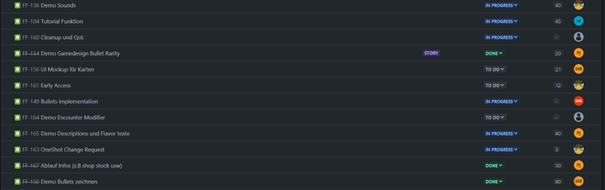
\includegraphics[width=\textwidth]{Backlog.png}
    \caption{Backlog}
\end{figure}

\subsection{Trello}\label{subsec:Trello}
%
Die Software Trello ist ein Projektmanagement Tool im Kanban Stil.
Es stellt ein Board dar, welches mit Karten befüllt wird.
Das Board ist in Spalten unterteilt, welche zur Kategorisierung oder zur Fortschrittseinteilung genutzt werden können.
Außerdem können Personen zu den Tasks zugewiesen werden, Aufwandseinschätzungen zugeordnet und Zeit getrackt werden.
Es ermöglicht eine einfache Übersicht durch die einfache simple Darstellung.

Das Team hat sich für Trello als internes Kanbanboard entschieden, da es damit aus vorherigen Projekten vertraut war und mit Jira nicht zurechtkam.
Einerseits ist Jira aus Sicht des Teams zu kompliziert und umfangreich.
Außerdem ist das Zeittracking in Jira mit Plugins wie Clockify äußerst umständlich und erschwert auch das mobile Zugreifen über das Telefon, während es eine Trello App gibt.
Das Zeittracking ist innerhalb von Trello mit dem Tool Everhour passiert und konnte den Aufgaben zugeordnet werden.

\begin{figure}[H]
    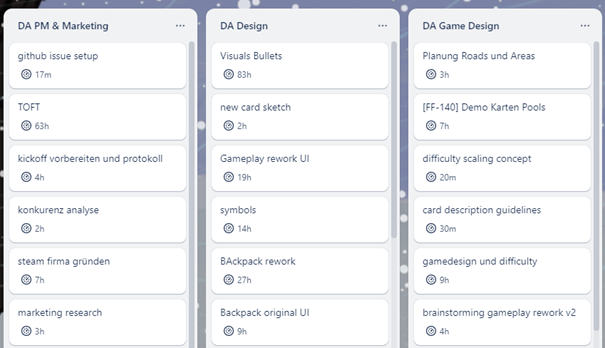
\includegraphics[width=\textwidth]{Trello_log.png}
    \caption{Trello}
\end{figure}
%
\subsection{Discord}\label{subsec:Discord}
Discord ist eine Kommunikationsplattform, die primär zur internen Kommunikation verwendet wurde, da sie viele Möglichkeiten der Kommunikation kombiniert.
Es sind sogenannte Voice Channels vorhanden, welche es den Teammitgliedern erlauben zusammen zu arbeiten und sich während der Arbeit auszutauschen.
Es gibt Textkanäle die zum Versenden von Nachrichten, Informationen oder Dateien ermöglichen.
Außerdem dient es als soziale Plattform, um sich eine Community aufzubauen.\zit{Discord}

Intern ist die Wahl auf Discord gefallen, da alle Teammitglieder mit der Plattform vertraut sind.
Außerdem bietet sie dem Team den notwendigen Umfang um die Zusammenarbeit zu vereinfach.
Sie verfügt über alle notwendigen Features wie Sprachkanäle mit Bildschirmübertragungsfunktion, Textkanäle und ist auf internen Austausch ausgelegt.

\begin{figure}[H]
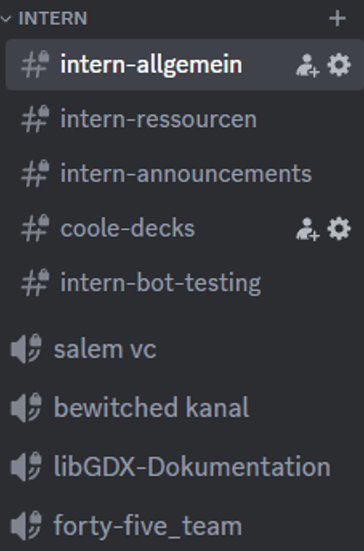
\includegraphics{Discord.png}\caption{Discord}
\end{figure}
%

% resets author
\renewcommand{\kapitelautor}{}


%
\chapter{Marketing}\label{ch:marketing}


\section{Zielgruppe}\label{sec:zielgruppe}

\renewcommand{\kapitelautor}{Autor: Nils Hubmann}

%
Die Einschätzung der Produktqualität und seines Erfolgs auf dem Markt hängt größtenteils vom Nutzen ab, den Kunden aus dem Produkt ziehen.
Es ist jedoch unerlässlich, dass das Produkt die Anforderungen, Wünsche und Erwartungen der Kunden optimal erfüllt, da sie letztendlich über den Erfolg eines Unternehmens entscheiden.
In diesem Zusammenhang sind Analysen wie die Definition der Zielgruppe äußerst hilfreich.
Unter dem Begriff Zielgruppenanalyse versteht man alle Aktivitäten, die damit einhergehen, zu verstehen, was die Konsumenten von einem Produkt erwarten, wie sie sich verhalten und welche Bedürfnisse sie haben.cite{Zielgruppe}


Die übliche Klassifizierung von Zielgruppen basiert oft auf äußeren Merkmalen, wie sozio-demografischen Daten oder finanziellen Aspekten.
Jedoch geht es bei der Definition einer Zielgruppe weit darüber hinaus.
Eine Zielgruppe zeichnet sich vor allem durch gemeinsame Wünsche, Bedürfnisse und Probleme aus.
Daher ist es wichtig, die Zielgruppe primär über ihre Bedürfnisse und Probleme zu definieren.
Erst danach können weitere übliche Kriterien wie Kaufkraft, Religion oder Alter zur weiteren Eingrenzung herangezogen werden. \zit{Zielgruppedef}

Dabei sind wir auf folgende Ergebnisse gekommen.

\subsubsection{Demographische Merkmale}\label{subsubsec:Demographische-Merkmale}

Die demografischen Merkmale beziehen sich auf das Alter, Geschlecht, Berufsstand und weiteren wichtigen Aspekte des täglichen Lebens.\zit{DemographischeMerkmale}

\begin{liste}
    \item Alter: 16-50 jährig (Das Spiel hat eine Altersbeschränkung von 16 Jahren)
    \item Geschlecht: Das Geschlecht ist nicht relevant
    \item Bildung: mittelmäßiges Bildungsniveau
    \item Beruf: Das Spiel ist für keine bestimmte Berufsgruppen interessant.
    \item Einkommen: Da das Spiel gratis sein wird, ist das Einkommen der Zielgruppe nicht relevant.
\end{liste}

\subsubsection{Geographische Merkmale}\label{subsubsec:Geographische-Merkmale}

„Auch diese Art von Merkmalen wird recht häufig genutzt, um zu erfahren, wo ihre Kunden wohnen, um so eine Werbung zu machen, welche auch die richtigen Leute am richtigen Ort trifft.“\zit{GeographischeMerkmale}
Die geografische Aufteilung nach Bundesländern oder Bezirken ist für dieses Computerspiel von geringer Bedeutung, da das Spiel global betrachtet wird und die Spielerbasis weltweit anspricht.
Die Kommunikation erfolgt hauptsächlich in englischer Sprache, um eine weitreichende Verständigung zu ermöglichen, insbesondere in englischsprachigen Ländern wie den USA, Großbritannien, Kanada und anderen.
Diese Länder werden aufgrund ihrer Muttersprache als Zielregionen betrachtet.

\subsubsection{Psychographische Merkmale}\label{subsubsec:Psychographische-Merkmale}

"Psychografische Faktoren sind beispielsweise Verhaltensmerkmale, Werte, Vorlieben und Charaktereigenschaften Ihrer Kunden und Kundinnen.
Welchen Lifestyle haben sie?
Was bewegt sie und warum?
Welchen Hobbys gehen sie in ihrer Freizeit nach?
Ist ein ausgeprägtes Gesundheits- und Umweltbewusstsein vorhanden?
Haben sie traditionelle Einstellungen oder
sind sie offen für Neues?
All diese Fragen helfen Ihnen, sich besser in Ihre Zielgruppe hineinzuversetzen." \zit{PsychographischeMerkmale}

\bold{Persönlichkeit:} Das Spiel ist hauptsächlich an Personen gerichtet, die sich für Karten- und Strategiespiele interessieren.

\bold{Freundesstand:} Da dieses Spiel allein spielbar ist, sind für die Nutzung keine weiteren Personen notwendig.

\bold{Hobby:} Computerspielen

Folgende Genres, die zur Bestimmung der Verhaltensweise wichtig sind:
\begin{liste}
    \item WildWest
    \item Strategie
    \item Indie
    \item Einzelspieler
    \item Roguelite
    \item Kostenlos
\end{liste}


\subsubsection{Zusammenfassung}\label{subsubsec:Zusammenfassung}
Das Spiel ist hauptsächlich für Hobbyspieler interessant, die nicht viel Geld in Spiele investieren wollen. Dabei hat \ff einen Vorteil gegenüber anderen Indiegames einen Vorteil,
da diese zwar nicht so viel kosten aber trotzdem nicht gratis sind.
Die meisten Indiegames kosten zwischen 5 und 25€ und sind daher Low Budget Games.\zit{IndiegamesPreis}
Des Weiteren wissen viele neue Spieler gar nicht, ob ihnen das Spiel gefällt, weshalb sie es, dadurch das es gratis ist, testen können.
Das kann wiederum dem Spiel helfen, mehr Aufmerksamkeit zu bekommen.


% resets author
\renewcommand{\kapitelautor}{}


\section{Social Media}\label{sec:social-media}

\renewcommand{\kapitelautor}{Autor: Nils Hubmann}


%
Social Media hat sich als unverzichtbares Werkzeug in der Vermarktung von Videospielen etabliert, und wir haben verschiedene Plattformen wie YouTube, Instagram und Reddit in Betracht gezogen, um die Reichweite unseres Spiels zu maximieren.
Besonders haben wir uns darauf konzentriert, mit YouTubern zusammenzuarbeiten, die durch ihre Videos unser Spiel einer breiten Zielgruppe vorstellen können.
Eine vielversprechende Entwicklung war die Kontaktaufnahme mit dem YouTuber Spieletrend, der positiv auf unsere Anfrage reagierte und sich bereit erklärte,
ein Video über unser Spiel zu erstellen und es ausführlich zu testen. Diese Zusammenarbeit verspricht nicht nur eine größere Sichtbarkeit, sondern auch authentische Einblicke und Bewertungen,
die das Interesse potenzieller Spieler wecken können. Zusätzlich haben wir unseren eigenen Content auf Social Media erstellt, um unsere Community zu engagieren und das Spiel bekannter zu machen.
Über unseren offiziellen Instagram-Account Microwavestudiosofficial wird Content aus dem Spiel, so wie das Team und der Trailer präsentiert, um das Interesse der Spieler zu wecken und die Vorfreude auf das Spiel zu steigern.
Auch über den Schul-Instagram-Account htl\_rennweg haben wir Content veröffentlicht, um Mitschüler für unser Spiel zu begeistern.
Darüber hinaus haben wir unsere Steam-Seite aktiv beworben und einen Trailer auf YouTube veröffentlicht, um potenzielle Spieler anzusprechen und einen ersten Eindruck von unserem Spiel zu vermitteln.
Die Nutzung verschiedener Social-Media-Plattformen bietet uns die Möglichkeit, direkt mit unserer Zielgruppe zu interagieren, Feedback zu erhalten und eine engagierte Community aufzubauen.
Durch die gezielte Zusammenarbeit mit Influencern und die aktive Einbindung unserer Community können wir das Interesse an unserem Spiel steigern und eine treue Fangemeinde aufbauen, die unser Spiel unterstützt und weiterempfiehlt.
%

\renewcommand{\kapitelautor}{}


\section{Website}\label{sec:website}
\renewcommand{\kapitelautor}{Autor: Nils Hubmann}

%
Die Webseite von \ff ist nicht nur ein digitaler Schauplatz und ausschlaggebend für die Bekanntmachung unseres Spiels

\bold{Promotion des Spiels:}
Eine Webseite ist von Bedeutung, um das Spiel einem breiteren Publikum bekannt zu machen.
Die Website wird auf diversen Social Media Kanälen beworben.
Durch die Präsentation von Screenshots, Trailern, Hintergrundgeschichten und Funktionen des Spiels können wir potenzielle Spieler ansprechen und ihr Interesse wecken.
Mit einer gut gestalteten und informativen Webseite können wir unsere Zielgruppe effektiv erreichen und das Spiel auf dem Markt positionieren.

\bold{Einblicke zum Spiel, dem Team und dem Projekt:}
Die Webseite bietet nicht nur Informationen über das Spiel selbst, sondern auch über das Team hinter dem Projekt.
Hierfür steht eine separate Projektseite zur Verfügung.
Indem wir Einblicke in das Projekt liefern, wollen wir die Seite als Möglichkeit nutzen und Leute auf die Idee aufmerksam machen.
Spieler können sich so besser mit dem Spiel identifizieren und eine emotionale Bindung dazu aufbauen.

\bold{Promotion der Steampage:}
Die Steampage ist das wichtigste Vertriebsmittel unseres Spiels und die Webseite dient als Sprungbrett, um Spieler dorthin zu führen.
Durch gezielte Verlinkungen und Trailer auf unserer Webseite
können wir die Neugier der Besucher wecken und sie dazu ermutigen, die Steampage zu besuchen.
Auf der Steampage finden sie dann detaillierte Informationen, Bilder und Videos, die ihr Interesse weiter vertiefen.
%

\vfill
\pagebreak

\subsection{Implementation}
\renewcommand{\kapitelautor}{Autor: Marvin Kurka}

Da es sich bei der Website um eine relativ simple, statische Website handelt, die kaum mit dem User interagiert,
wurde die Entscheidung getroffen kein Framework wie \zB Vue oder React zu verwenden.
Allerdings wurde Sass verwendet, eine Css-Extension, die mehrere Features hat, die das Erstellen und Strukturieren
von großen Stylesheets vereinfachen.
Sass erlaubt \zB das Verwenden von Variablen, das Unterordnen von Selektoren oder das Aufteilen von
Stylesheets in mehrere Dateien.\zit{sassDoc}
Da ein relativ umfangreiches Stylesheet für die Website notwendig war, wurde die Entscheidung getroffen Sass zu
verwenden, um die Wartbarkeit zu erhöhen.

Eine weitere Eigenschaft der \FF Website ist, dass besonders viele Bilder verwendet werden, um die Website dem Stil des
Spiels anzugleichen.

\begin{figure}[H]
    \centering
    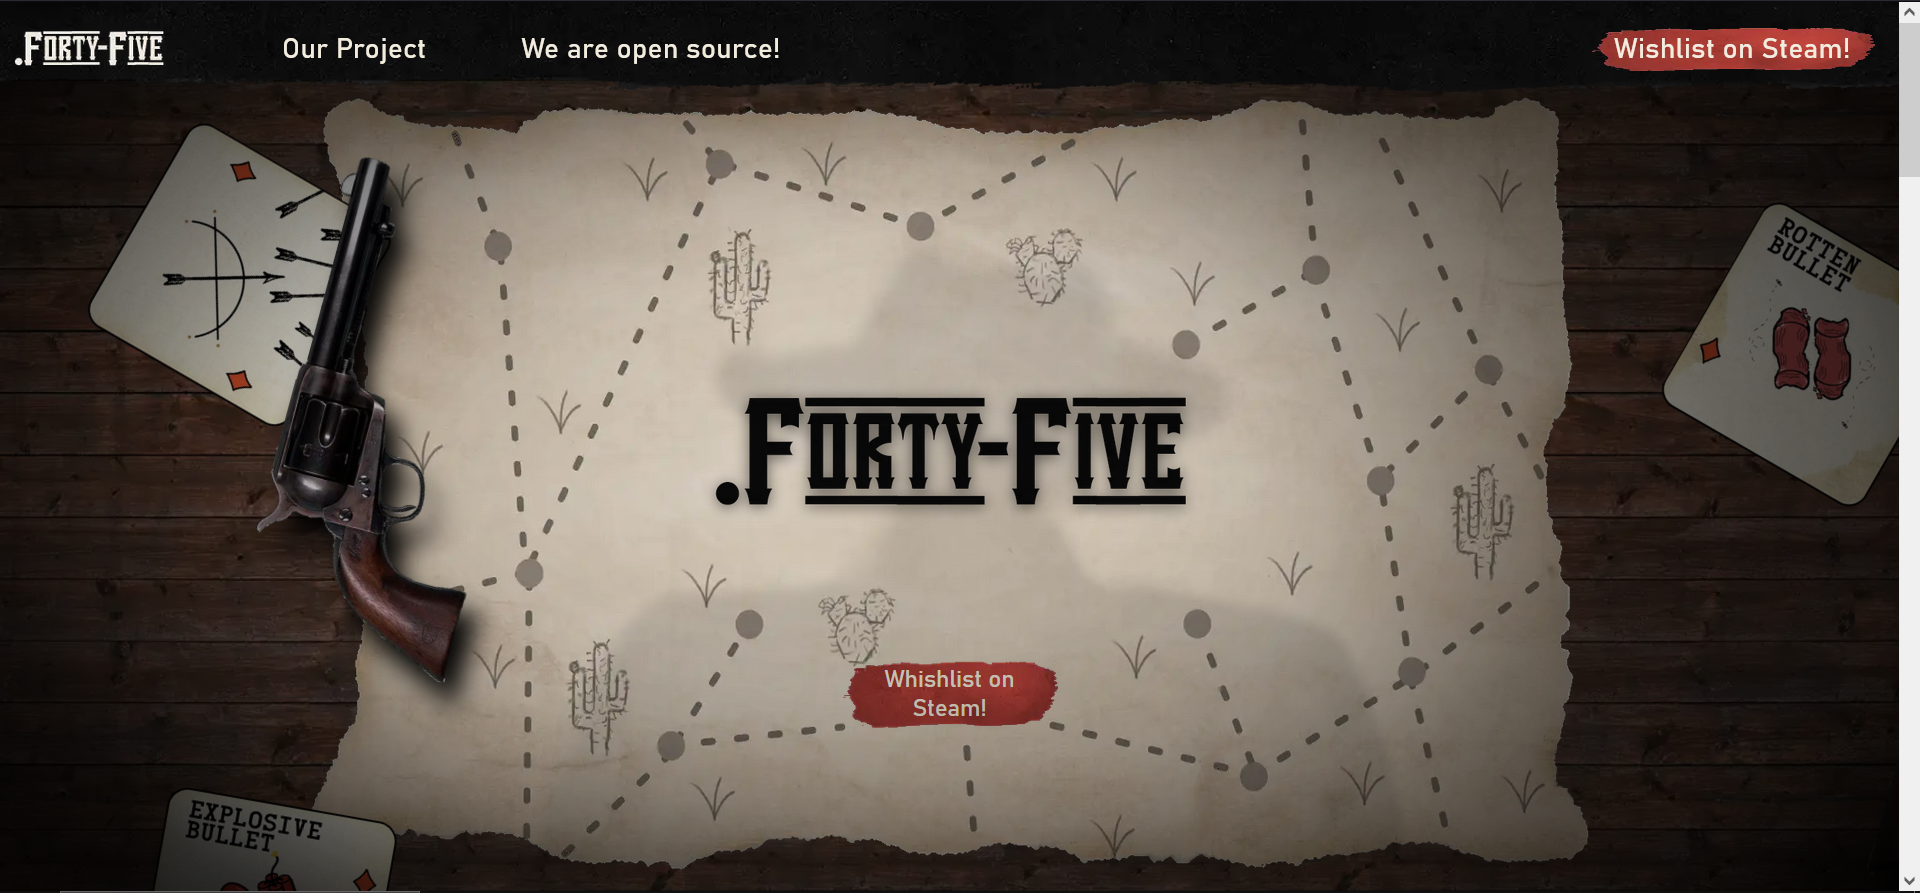
\includegraphics[width=1.0\textwidth]{website.png}
    \caption{Screenshot der Website}
\end{figure}

Das wirkt sich negativ auf die Ladezeiten der Website aus.
Um diesen Effekt so gering wie möglich zu halten, wurde das von Google entwickelte webp Bild-Format verwendet, welches
eine deutlich bessere Komprimierung als vergleichbare Formate wie \zB jpg erzielt.
In einer vergleichenden Studie, welche von Google durchgeführt wurde, erreichte webp je nach verwendeter Methodik eine
Verkleinerung von 14\% gegenüber eines mit jpg komprimierten Bildes.\zit{googleWebpStudie}

\vfill
\pagebreak

% resets author
\renewcommand{\kapitelautor}{}


\section{Trailer}\label{sec:trailer}

\renewcommand{\kapitelautor}{Autor: Markus Böheim}

Für den Trailer wird Adobe Premiere Pro verwendet. Das Hauptziel des Trailers ist es das Gameplay actionreich zu präsentieren, damit es Interesse weckt und um die Grafiken hervorzuheben. Die Zielgruppe von Forty-Five sind junge Menschen die bereits Interesse an dem Genre haben, also muss ein gewisser Vergleich oder Ähnlichkeit im Trailer zu anderen Spielen in diesem Genre sein, damit der Spieler weiß, worum es geht. Eine Grobe Idee für den Trailer oder Skript in Form eines Storyboards, sorgt bei der Umsetzung des Trailers für einen schnelleren Workflow sowohl bei der Pre-Production als auch bei dem Zusammenschnitt. Als Referenz wird der Trailer von „Slay the Spire“ vorgenommen, um einen Anhaltspunkt für die Geschwindigkeit zu haben. Zuerst werden mit dem Storyboard die notwendigen Szenen aufgenommen. Dafür wird eine Version des Spiels benötigt ohne Musik, da diese beim Schnitt Probleme bereitet. Nach der Aufnahme werden nach der Anleitung des geschriebenen Storyboards die aufgenommenen Clips zusammengeschnitten. Zooms helfen, um mehr Fokus auf eine bestimme Aktion oder ein Objekt zu bringen. Keyframes – auf Deutsch Schlüsselbilder – Keyframes legen Start- und Endpunkt einer Animation fest. Mit Keyframes ist es möglich, einen Zoom Effekt in Schnittprogrammen zu erstellen, indem man beispielsweise einen Startpunkt mit der Skalierung 100 und einen Endpunkt mit der Skalierung 110 setzt. Das ist allerdings nur eine lineare Kurve, die unnatürlich aussieht. Mit Ease-In und Ease-Out Funktionen wird das Skalieren dadurch natürlicher, welche per Rechtsklick auf den Keyframe eingestellt werden können.

\begin{figure}[H]
    \centering
    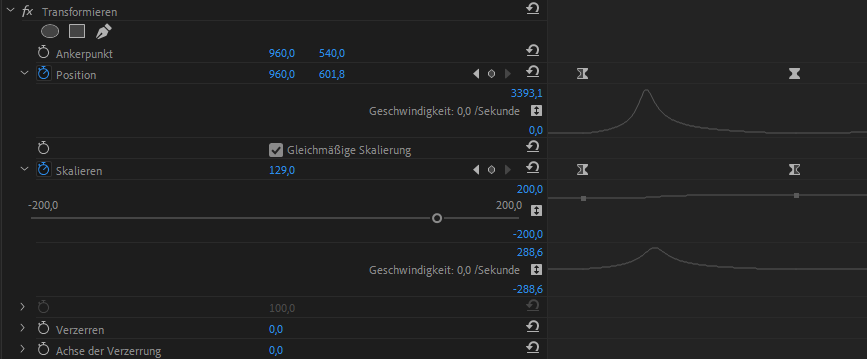
\includegraphics[width=0.6\textwidth]{easeInOut.png}
    \caption{Ease-In/Out Zoom im Trailer}
\end{figure}

Die Musik im Trailer ist lizenzfrei unter dem Link \url{https://www.youtube.com/watch?v=KIhO3u0xuhQ} zu finden und wird gewählt, da die Instrumente und Soundgeräusche zum wilden Westen passen und eine dramatische, ernste Stimmung hat. Da der Trailer nur grob eine Minute lang ist und das Musikstück grob drei Minuten lang ist, muss der Song auf den Trailer angepasst werden. Premiere Pro bietet eine „Remix“ Funktion, welche unter dem „Essential Sound“ Reiter zu finden ist, die es einem erlaubt, die Länge eines Songs anzupassen, ohne dass der Rhythmus des Songs dabei unterbrochen wird.

\begin{figure}[H]
    \centering
    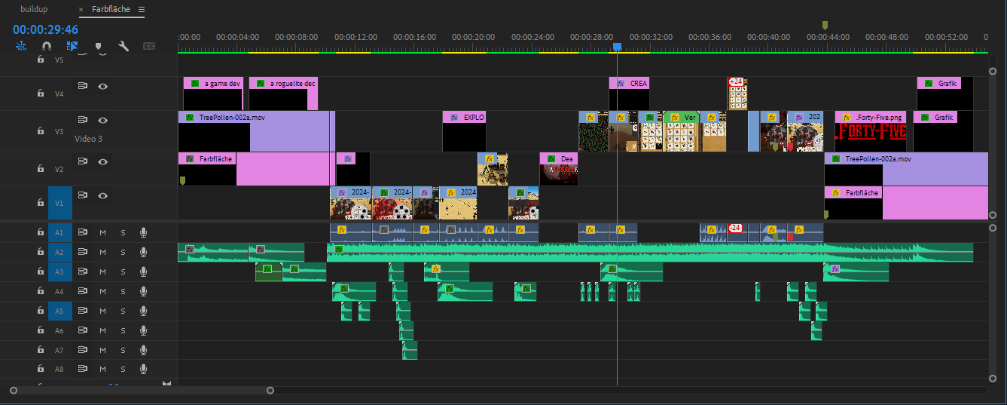
\includegraphics[width=0.6\textwidth]{schnittfenster.png}
    \caption{Arbeitsfläche des Trailers}
\end{figure}

Das Audio beziehungsweise die Vertonung ist genauso wichtig, wie das Video an sich selbst. Für Texte, die erscheinen, wird ein Soundeffekt verwendet, welcher einem wischen ähnelt. Die Sounds für den Trailer werden von Pixabay’s kosten- und lizenzfreier Audiobibliothek genommen und werden von der Lautstärke so angepasst, dass diese mit den anderen Audiospuren inklusive des Musikstücks den Richtwert -6dB nicht überschreiten. Dieser Audiopegel von -6dB sorgt dafür, dass das Audio ausreichend „Headroom“ beziehungsweise Spielraum hat, um plötzliche Laute Geräusche abzufangen, ohne dass diese übersteuern. Abschließend wird der Trailer in 1080p und 60 Bildern pro Sekunde exportiert, mit einer Bitrate von 36Mbit/s, um das Video konform für die Veröffentlichung in sozialen Medien zu machen. Die Bitrate sagt aus, wie viele Daten pro Sekunde übertragen werden, was die Qualität und Dateigröße beeinflusst.



% resets author
\renewcommand{\kapitelautor}{}


%
\chapter{Kotlin}\label{ch:kotlin}


\section{Code Clarity}\label{sec:code-clarity}

\renewcommand{\kapitelautor}{Autor: Irgendwer} % todo: replace

%
% text goes here
%

% resets author
\renewcommand{\kapitelautor}{}


\section{Null Safety}\label{sec:null-safety}

\renewcommand{\kapitelautor}{Autor: Irgendwer} % todo: replace

%
% text goes here
%

% resets author
\renewcommand{\kapitelautor}{}


\section{Flow Typing}\label{sec:flow-typing}

\renewcommand{\kapitelautor}{Autor: Irgendwer} % todo: replace

%
% text goes here
%

% resets author
\renewcommand{\kapitelautor}{}


\section{Lambdas}\label{sec:lambdas}

\renewcommand{\kapitelautor}{Autor: Marvin Kurka}

\subsection{Lambdas in Java und Javascript}
Anders als Kotlin wurde Java ursprünglich ohne Lambdas entwickelt, diese wurden erst in der Version Java 8 hinzugefügt.
Durch diesen Umstand entstand eine wesentliche Limitation der Java Lambdas, nämlich den Fakt das Closures nicht
funktionieren wie man es von anderen Sprachen wie \zB Javascript erwartet.
Generell ist es so, das ein Lambda Werte, die in äußeren Scopes definiert wurden in einer sogenannten Closure captured
und so weiter sowohl lesend als auch schreibend auf diese zugreifen kann.
Java allerdings erlaubt nur den lesenden Zugriff, und nur wenn auch Code außerhalb des Lambdas niemals schreibend auf
die Variable zugreift.\cite{mdnDocsClosures, jarticleLambdas}

\begin{minted}{javascript}
function createClosure() {
    let i = 0;
    const getter = () => i;
    const setter = value => { i = value; };
    return [getter, setter];
}
const [getter, setter] = createClosure();
setter(10);
console.log(getter()); // => 10
setter(getter() * 2);
console.log(getter()); // => 20
\end{minted}
\codeblockCaption{Demonstration von closures in Javascript}

\begin{minted}{java}
int i = 0;
String effectivelyFinal = "hi";
AtomicInteger a = new AtomicInteger(0);
Runnable r = () -> {
    i++; // compile time fehler
    a.incrementAndGet(); // workaround mit AtomicInteger, funktioniert
    System.out.println(effectivelyFinal); // erlaubt, weil effectivelyFinal nie zugewiesen wird
};
\end{minted}
\codeblockCaption{Demonstration von limitierten closures in Java}

Kotlin wurde anders als Java von Anfang an mit Lambdas entwickelt und weist daher keine solchen Limitationen auf.
Da Kotlin sich selbst als Sprache mit vielen Elementen aus der funktionalen Programmierung bezeichnet, ist es wichtig,
dass Lambdas und Closures so funktionieren wie erwartet und gut in die Sprache integriert sind.\cite{kspecIntroduction}

\subsection{Lambda Syntax in Kotlin}
Ein Aspekt der Kotlins Lambdas von Lambda-Implementation in anderen Sprachen besonders unterscheidet ist der Syntax.
Eine geschwungene Klammer, die frei im Code auftaucht, eröffnet nicht wie anderen Sprachen wie \zB Java oder Javascript
einen neuen Code-Block, sondern deklariert ein Lambda.
Lambda Parameter werden in den geschwungenen Klammern angegeben.\cite{kspecLambdaLiteral}

%! language = kotlin
\begin{minted}{kotlin}
fun test() {
    {
        println("hi")
    }
}
\end{minted}
\codeblockCaption{
Das hier gezeigte \inlineKotlin{println()} wird nie tatsächlich ausgeführt, das es in einem Lambda
definiert wurde, das selbst nie ausgeführt wird
}

%! language = kotlin
\begin{minted}{kotlin}
fun test() {
    val lambda: (String) -> Unit = { string -> println(string) }
    lambda("hello")
    lambda("world")
}
\end{minted}
\codeblockCaption{Lambda-Literal mit einem Parameter}

Zusätzlich stellt Kotlin einige syntaktische Vereinfachen zur Verfügung, wenn eine Funktion als letzten Parameter
ein Lambda nimmt.
In diesem Fall kann das Lambda nämlich außerhalb der Klammern des Funktionsaufrufs geschrieben werden.

%! language = kotlin
\begin{minted}{kotlin}
fun test() {
    // repeat ist keine Control-Flow-Struktur, sondern eine normale Funktion, die in der
    // Standard-Bibliothek definiert ist.
    repeat(5) {
        println("hi")
    }
}
\end{minted}
\codeblockCaption{Demonstration von einem Funktionsaufruf mit Lambda}

Wenn die Funktion sonst keine Parameter nimmt, können die Klammern sogar komplett weggelassen werden.

%! language = kotlin
\begin{minted}{kotlin}
fun test() {
    run {
    }
    // ist gleich
    run() {
    }
    // ist gleich
    run({ })
}
\end{minted}

\inlineKotlin{run} ist eine Funktion aus der Standard-Bibliothek, die ein Lambda entgegennimmt und einmal ausführt.
Diese Funktion wird in der Praxis verwendet, um normal Code-Blöcke zu ersetzen.

Achtung!
Ist eine geschwungene Klammer Teil einer syntaktischen Struktur eröffnet sie einen normalen Code-Block, kein Lambda!

%! language = kotlin
\begin{minted}{kotlin}
fun test() {
    if (someCondition) { // Diese geschwungene Klammer eröffnet kein Lambda!
    }
}
\end{minted}

Eine weitere Vereinfachung ist, dass ein Lambda, das nur einen Parameter nimmt, diesen nicht explizit angeben muss.
Stattdessen wird implizit eine lokale Variable namens \inlineKotlin{it} erschaffen.
Das erleichtert vor allem lange Aufrufketten auf Iterables.

%! language = kotlin
\begin{minted}{kotlin}
data class Country(val name: String, val population: Int)
fun test() {
    val countries = listOf<Country>()
    // erstellt einen String mit den Anfangsbuchstaben aller Länder mit mehr als 500 Einwohnern die mit "land" enden
    val result = countries
        .filter { it.population > 500 }
        .map { it.name }
        .filter { it.endsWith("land") }
        .map { it.first() }
        .fold("") { acc, cur -> acc + cur }
}
\end{minted}
\codeblockCaption{Praxisnahes Beispiel für Lambdas}

Wie im letzten Beispiel ersichtlich, ist es nicht notwendig explizit eine \inlineKotlin{return} expression in einem
Lambda zu verwenden.
Stattdessen wird der Wert der letzten Expression im Block automatisch als return-Wert angenommen.

%! language = kotlin
\begin{minted}{kotlin}

enum class ColorMode { LightMode, DarkMode }
data class UserPrefs(val selectedColorMode: ColorMode?)
data class Defaults(val defaultColorMode: ColorMode = ColorMode.DarkMode)

fun test() {
    val colorPicker: (UserPrefs, Defaults) -> String = { prefs, defaults ->
        val colorMode = prefs.selectedColorMode ?: defaults.defaultColorMode
        when (colorMode) { // when ist die letzte Expression im Lambda, daher wird ihr Wert als return-Wert genommen
            ColorMode.LightMode -> "#ffffff"
            ColorMode.DarkMode -> "#000000"
        }
    }
}
\end{minted}

% resets author
\renewcommand{\kapitelautor}{}


\section{Nothing Typ}\label{sec:nothing-type}

\renewcommand{\kapitelautor}{Autor: Marvin Kurka}

Der \inlineKotlin{kotlin.Nothing} Typ ist in der Kotlin Standard-Bibliothek definiert, er hat allerdings einige
spezielle Eigenschaften.
Zum Beispiel handelt sich bei Nothing um einen unified subtype (auch bottom Type genannt) für alle in Kotlin
definierten Typen.
Das heißt, eine Instanz von Nothing wäre auch eine Instanz jeder anderen Klasse, sei es \inlineKotlin{String},
\inlineKotlin{Int} oder \inlineKotlin{() -> Boolean}.
Da so ein Objekt einen logischen Widerspruch darstellt, handelt es sich bei Nothing auch um einen uninhabited Type.
Das heißt, dass niemals eine tatsächliche Instanz von Nothing existieren kann.

Auf den ersten Blick mag so ein Typ nicht sehr nützlich wirken, er erlaubt den Compiler aber einige nützliche
Annahmen über den Control Flow zu machen.
Sollte jemals eine Variable den Wert Nothing annehmen, was einen logischen Widerspruch darstellt, weiß der Compiler,
dass dieser Code niemals erreicht werden kann.\cite{kspeCFG,kspecNothing}

%! language = kotlin
\begin{minted}{kotlin}
fun getNothing(): Nothing {
    ...
}

fun test() {
    // Nothing ist ein Subtype von String, daher ist der folgende Code erlaubt
    val s: String = getNothing()

    // für diesen Code gibt der Compiler eine Warning aus, da er niemals erreicht werden kann
    println("Hello World")
}
\end{minted}
\codeblockCaption{
Dadurch das die Funktion \inlineKotlin{getNothing()} den Rückgabewert Nothing hat, der niemals existieren kann,
weiß der Compiler, dass diese Funktion niemals auf normale Art und Weise returnen kann und in einer Exception
resultieren muss.
}

Um den Nothing-Typen tatsächlich nützlich zu machen, sind in Kotlin Statements, die einen Control-Flow Transfer
verursachen eigentlich Expressions mit dem Rückgabewert Nothing.
Beispiele sind: \inlineKotlin{throw}, \inlineKotlin{return}, \inlineKotlin{break} und \inlineKotlin{continue}.
Da diese Expressions einen sofortigen Wechsel des Control-Flows verursachen hat das zur Folge, dass der nachfolgende
Code niemals ausgeführt wird.
Damit können diese Expressions den Wert Nothing haben.\cite{kspeCFG}

%! language = kotlin
\begin{minted}{kotlin}
operator fun Int?.plus(other: Int?): Int? {
    // return hat den Wert Nothing, was ein Subtype von Int ist,
    // daher ist die Verwendung nach dem elvis operator erlaubt
    val first = this ?: return null
    val second = other ?: return null
    return first + second
}
\end{minted}
\codeblockCaption{Praktisches Beispiel für die Verwendung des Nothing-Typen}

Dadurch das \inlineKotlin{return} in Kotlin eine Expression ist, ist auch der folgende Code gültiges Kotlin:

%! language = kotlin
\begin{minted}{kotlin}
fun test() {
    println("Hello")
    return return return return return
}
\end{minted}

Funktionen, die den Rückgabewert Nothing haben, müssen immer eine Exception werfen.

%! language = kotlin
\begin{minted}{kotlin}
fun crashProgram(cause: String): Nothing {
    MyLogger.log("Program crashed because of: $cause")
    throw RuntimeException(cause)
}

fun doSomething(input: String?) {
    otherFunction(input ?: crashProgram("input must not be null"))
}
\end{minted}

Ein Beispiel für eine Funktion aus der Kotlin Standard-Bibliothek die Nothing zurückgibt, ist die
\inlineKotlin{TODO()} Funktion.

%! language = kotlin
\begin{minted}{kotlin}
fun someFunction(): Int = TODO("not yet implemented")
\end{minted}

Ein weiterer Anwendungsfall von Nothing ist als generischer Parameter, um \zB eine leere Liste zu signalisieren.
Eine \inlineKotlin{List<Nothing>} muss immer leer sein, da keine Instanz von Nothing existieren kann.

% resets author
\renewcommand{\kapitelautor}{}


\section{Extension Functions}\label{sec:extension-functions}

\renewcommand{\kapitelautor}{Autor: Irgendwer} % todo: replace

%
% text goes here
%

% resets author
\renewcommand{\kapitelautor}{}


\section{Inline Functions}\label{sec:inline-functions}

\renewcommand{\kapitelautor}{Autor: Marvin Kurka}

\subsection{inline Funktionen in anderen Sprachen}
In C/C++ werden von den Compilern häufig kurze Funktionen geinlined.
Das heißt, der Funktionsaufruf wird mit den tatsächlichen Body der Funktion ersetzt, und kein tatsächlicher
Funktionsaufruf findet statt.
C und C++ haben den \inlineCode{inline} Modifier, der als Hinweis für den Compiler dient, dass diese Funktion
geinlined werden soll.
Der Compiler darf allerdings selber entscheiden, ob er das tut \bzw auch nicht mit \inlineCode{inline} markierte
Funktionen inlinen.
Der Grund für Funktions-inlining ist in erster Linie Performance, da dadurch ein Funktionsaufruf gespart wird.\cite{crefInline}

In Kotlin ist der Grund für Funktions-inlining explizit nicht um den Overhead eines Funktionsaufrufs zu sparen,
der Compiler warnt sogar, wenn der \inlineKotlin{inline} Modifier verwendet wird und kein sonstiger Grund für
inlining besteht.

\subsection{Effizientere Lambdas}
Dieser Abschnitt hat nur für Kotlin/JVM Gültigkeit.
Auf anderen Plattformen wie native, js oder wasm könnte sich der Compiler anders verhalten.

Eine Anwendung für inline-Funktionen sind higher-order-functions, also Funktionen, die andere Funktionen als Parameter
nehmen.
Im Normalfall muss der Compiler für das Lambda eine anonyme Klasse generieren, die da Lambda enthält, und alle Variablen,
die Teil der Closure sind, speichern.
Wenn eine solche Funktion als \inlineKotlin{inline} markiert ist, kann der Compiler nicht nur die Funktion, sondern auch
das Lambda inlinen, was diesen Overhead spart.

Beispiel für higher-order inline Funktionen:

%! language = kotlin
\begin{minted}{kotlin}
fun runLambda(lambda: () -> Unit) = lambda()
inline fun runLambdaInline(lambda: () -> Unit) = lambda()

fun test() {
    runLambda {
        println("runLambda")
    }
    runLambdaInline {
        println("runLambdaInline")
    }
}
\end{minted}

Dieser Code wurde mit kotlinc-jvm 1.9.21 compiled und mit javap 14.0.2 disassembled.
Unten ist die Disassembly der test-Funktion zu sehen.

\begin{minted}{text}
 0: getstatic     #34                 // Field TestKt$test$1.INSTANCE:LTestKt$test$1;
 3: checkcast     #18                 // class kotlin/jvm/functions/Function0
 6: invokestatic  #36                 // Method runLambda:(Lkotlin/jvm/functions/Function0;)V
 9: iconst_0
10: istore_0
11: iconst_0
12: istore_1
13: ldc           #37                 // String runLambdaInline
15: getstatic     #43                 // Field java/lang/System.out:Ljava/io/PrintStream;
18: swap
19: invokevirtual #49                 // Method java/io/PrintStream.println:(Ljava/lang/Object;)V
22: nop
23: nop
24: return
\end{minted}

Wie in der Disassembly zu sehen ist, hat der Compiler für das erste Lambda (Offset 0--8) eine eigene Klasse
(TestKt\$test\$1) erstellt.
Da das Lambda in diesem Fall keine Variablen in einer Closure speichert, kann der Compiler ein Singleton generieren,
was zumindest den Konstruktor-Aufruf spart.
Wie von Offset 12--21 zu sehen ist, wird das \inlineKotlin{println} der zweiten direkt in der test-Funktion
aufgerufen, da das Lambda geinlined wurde.

\begin{infoBox}
In der Disassembly sind auch mehrere merkwürdige Instruktionen zu sehen, \zB von Offset 9--12 oder von 22--23.
Diese sind Anhang\ref{ch:anhang-1} erklärt.
\end{infoBox}

% resets author
\renewcommand{\kapitelautor}{}


\section{Getter und Setter}\label{sec:getter-und-setter}

\renewcommand{\kapitelautor}{Autor: Irgendwer} % todo: replace

%
% text goes here
%

% resets author
\renewcommand{\kapitelautor}{}


\section{Kotlin vs. Java}\label{sec:kotlin-vs-java}

\renewcommand{\kapitelautor}{Autor: Irgendwer} % todo: replace

%
% text goes here
%

% resets author
\renewcommand{\kapitelautor}{}


%
\chapter{Tools}\label{ch:tools}


\section{Git}\label{sec:git}

\renewcommand{\kapitelautor}{Autor: Irgendwer} % todo: replace

\subsection{Workflow}\label{subsec:workflow}

%
% text goes here
%

\subsection{Github}\label{subsec:github}

%
% text goes here
%

% resets author
\renewcommand{\kapitelautor}{}


\section{Onj}\label{sec:onj}

Onj ist eine selbst entwickelte Markupsprache, die Ähnlichkeiten zu Sprachen wie Json, Toml oder Yaml aufweist,
diese allerdings um einige Features erweitert.
Onj-Dateien sind dafür ausgelegt, von Hand geschrieben zu werden und haben daher einige Quality of Life Features, die
ähnliche Sprachen nicht aufweisen.
Außerdem soll Onj auch für größere Projekte geeignet sein, ohne das der Wartungsaufwand zu groß wird.
Daher hat Onj Mechanismen um repetitiven Code zu vermeiden, wie imports oder Variablen, die Möglichkeit Strukturen
mit Schemas zu validieren und die Fähigkeit mittels Namespaces mit Kotlin-Code zu interagieren.

Onj-Dateien können nicht nur von Programmen eingelesen werden, Onj-Strukturen können auch mittels der
\inlineKotlin{buildOnjObject}-Funktion im Programm gebaut und in Dateien geschrieben werden.
Dabei können die Strukturen nicht nur zu gültigen Onj, sondern auch zu Json serialisiert werden.


\subsection{Warum Onj?}\label{subsec:warum-onj}

\renewcommand{\kapitelautor}{Autor: Marvin Kurka}

Erfahrung, die wir in früheren Projekten \bzw Vorarbeit an \FF gesammelt haben zeigt, dass
es oft kurzfristig zu Änderungen und Anpassen bezüglich des Gameplays kommt.
Oft handelt es sich dabei um komplexere Funktionen, die Mechaniken des Gameplays ändern, oft sind es aber auch nur
simple Balancing-Änderungen, wo \zB nur der Schadenswert einer Karte geändert wird.
Daher hatten wir bei \FF den Anspruch, dass solche Balancing-Änderungen schnell und von Leuten mit keiner Kenntnis
des Programmaufbaus vorgenommen werden können.

Bei der Wahl der Markupsprache hatten wir die Wahl zwischen einen bereits etablierten Format wie XML, JSON oder YAML,
oder den selbst entwickelten Format Onj.
Unsere Wahl ist aus mehreren Gründen auf Onj gefallen.

\begin{itemize}
    \item Variablen und Imports erhöhen die Maintainability in größeren Projekten
    \item OnjSchemas helfen sicherzustellen, das die Dateien im korrekten Format sind
    \item Onjs Syntax ist leichter zu lesen als \zB der von Json
    \item Namespaces ermöglichen eine gute Integration mit dem Programm
    \item Onjs API ist für Kotlin ausgelegt und verwendet Features der Sprache, wie reified Generics oder
        Lambdas mit Receiver
    \item Dadurch, dass Onj selbst entwickelt wurde, können, falls notwendig, Features hinzugefügt werden (So wurde die
        Sprache \zB während des Projektes um einen Minifier erweitert, um Maps effizienter zu speichern.)
\end{itemize}

% resets author
\renewcommand{\kapitelautor}{}

\input{text/06_tools/02_onj/02_überblick_syntax.tex}

\subsection{Variablen}\label{subsec:variablen}

\renewcommand{\kapitelautor}{Autor: Marvin Kurka}

Um das Wiederholen von Code so gering wie möglich zu halten, werden in Onj Variablen verwendet, um häufige Strukturen
zu extrahieren.
Mittels des Variablennamen kann dann auf diese zugegriffen werden, auch Verknüpfungen mit Punkten sind erlaubt.

%! language = Onj
\begin{codeBlock}{onj}{Beispiel: Variablen in Onj}
var number = 5;
favoriteNumber: number,
otherNumber: (number + 1) * number,

var colors = {
    red: "#ff0000",
    green: "#00ff00",
    blue: "#0000ff",
};
favoriteColor: colors.blue,

var fruits = ["apple", "banana", "grape"];
// auf arrays wird mittels des Indexes zugegriffen
favoriteFruit: fruits.0,
\end{codeBlock}

Es können auch drei Punkte verwendet werden, um den Inhalt einer Variable in die aktuelle Struktur zu übernehmen.

%! language = Onj
\begin{codeBlock}{onj}{Beispiel: Triple-Dot Syntax in Onj}
var fruits = ["apple", "pear"];
fruitSalad: [
    "banana",
    "grape",
    ...fruits
],
\end{codeBlock}

Statt bei einem Zugriff einfach den Key-Namen oder den Index anzugeben, kann auch in Klammern eine Expression angegeben
werden.
Diese wird evaluiert und das Resultat wird für den Zugriff verwendet.

%! language = Onj
\begin{codeBlock}{onj}{Demo: dynamische Zugriffe in Onj}
var index = 1;
var arr = [0, 1, 2, 3, 4, 5];
myValue: arr.(index + 2) // => 3
\end{codeBlock}

% resets author
\renewcommand{\kapitelautor}{}


\subsection{Imports}\label{subsec:imports}

\renewcommand{\kapitelautor}{Autor: Marvin Kurka}

Oft ist es so, dass gewisse Strukturen öfter verwendet werden müssen.
Das kann Probleme mit der maintainability verursachen, da, falls eine Änderung vorgenommen wird, diese dann an vielen
Stellen repliziert werden muss.
Um solche Redundanzen innerhalb einer Datei zu vermeiden können Variablen verwendet werden, oft treten jedoch auch
dateiübergreifende Redundanzen auf.
Import-Statements erlauben häufige Strukturen in eine eigene Datei auszulagern und diese dann in anderen Dateien zu
importieren.
Bei einem Import-Statement wird neben dem Pfad der zu importierenden Datei auch ein Variablenname angegeben, unter dem
dann eine Variable mit dem Inhalt der importierten Datei erschaffen wird.

%! language = Onj
\begin{minted}{onj}
// toImport.onj
myValue: 5
\end{minted}

%! language = Onj
\begin{minted}{onj}
// importer.onj
import "toImport.onj" as imported;
importedValue: imported.myValue,
\end{minted}

Der Pfad kann, ähnlich wie ein Variablenzugriff, dynamisch gemacht werden.
Dazu werden Klammern verwendet.

%! language = Onj
\begin{minted}{onj}
var colorSchemes = ["lightMode.onj", "darkMode.onj"];
import "userPrefs.onj" as userPrefs;
import (colorSchemes.(userPrefs.preferredColorScheme)) as colorScheme;
\end{minted}

% resets author
\renewcommand{\kapitelautor}{}


\subsection{Onj Schemas}\label{subsec:onj-schemas}

\renewcommand{\kapitelautor}{Autor: Irgendwer} % todo: replace

%
% text goes here
%

% resets author
\renewcommand{\kapitelautor}{}


\subsection{Named Objects}\label{subsec:named-objects}

\renewcommand{\kapitelautor}{Autor: Irgendwer} % todo: replace

%
% text goes here
%

% resets author
\renewcommand{\kapitelautor}{}


\subsection{Namespaces}\label{subsec:namespaces}

\renewcommand{\kapitelautor}{Autor: Marvin Kurka}

Namespaces erlauben es, Onj zu erweitern, indem eigene Funktionen, zusätzliche globale Variablen oder
eigene Datentypen definiert werden.
Solche Namespaces werden in Kotlin definiert und mit Annotations markiert.

Funktionen werden im Namespace definiert und mit der \inlineKotlin{@RegisterOnjFunction} markiert.
Diese Annotation nimmt ein String mit einem OnjSchema als Parameter, der die Signatur der Funktion beschreibt.
Das ist notwendig, da Onj das Überladen von Funktionen erlaubt, \dah mehrere Funktionen dürfen denselben Namen haben.
Um herauszufinden, welche Funktion tatsächlich aufgerufen werden soll, vergleicht der Onj-Parser die mitgegebenen
Parameter mit dem Schema und ruft die erste Funktion auf, bei der diese übereinstimmen.

%! language = Kotlin
\begin{codeBlock}{kotlin}{Demo: Deklaration einer Onj-Funktion in Kotlin}
@OnjNamespace
object MyNamespace {

    @RegisterOnjFunction(schema = "params: [string, int]")
    fun repeatString(s: OnjString, times: OnjInt) = OnjString(s.value.repeat(times.value))
}
\end{codeBlock}

Neben normalen Funktionen stellt Onj noch drei spezielle Arten von Funktionen zur Verfügung:

\begin{liste}
    \item Conversions: Diese werden mit folgendem Syntax aufgerufen: \inlineOnj{value#function}.
        Solche Funktion werden zum Beispiel verwendet, um einen Wert von einem Datentypen zu einem anderen zu
        konvertieren.
    \item Infix Funktionen: Diese werden mit folgendem Syntax aufgerufen: \inlineOnj{value1 function value2}.
        Beispiele sind die pow-Funktion (\inlineOnj{10 pow 5}) oder die in-Funktion (\inlineOnj{3 in [1, 2, 3, 4]}).
    \item Operator Overloading: Solche Funktionen erlauben es zu definieren, wie sich Operatoren wie
        \inlineOnj{+} oder \inlineOnj{*} für eigene Datentypen verhalten.
\end{liste}

Wird so eine spezielle Funktion verwendet, wird das in der \inlineKotlin{@RegisterOnjFunction} Annotation angegeben.

%! language = Kotlin
\begin{codeBlock}{kotlin}{Demo: Deklaration einer Onj-Conversion in Kotlin}
@OnjNamespace
object MyNamespace {

    @RegisterOnjFunction(schema = "params: [string]", type = OnjFunctionType.CONVERSION)
    fun greeting(name: OnjString) = OnjString("Hello, ${name.value}")
}
\end{codeBlock}

Weiters können Namespaces globale Variablen definieren.

%! language = Kotlin
\begin{codeBlock}{kotlin}{Demo: Deklaration von globalen Onj-Variablen in Kotlin}
@OnjNamespace
object MyNamespace {

    @OnjNamespaceVariables
    val variables: Map<String, OnjValue> = mapOf(
        "myGlobal" to OnjInt(5)
    )
}
\end{codeBlock}

In Onj kann ein use-Statement verwendet werden, um einen Namespace zu inkludieren.

%! language = Onj
\begin{codeBlock}{onj}{Demo: Verwendung eines Onj-Namespaces}
use MyNamespace;

global: myGlobal,
greeting: "Reader"#greeting,
string: repeatString("a", 5)
\end{codeBlock}

% resets author
\renewcommand{\kapitelautor}{}



\renewcommand{\kapitelautor}{Autor: Felix Zwickelstorfer}
\section{Gradle}\label{sec:gradle}

\renewcommand{\kapitelautor}{Autor: Felix Zwickelstorfer}

Gradle ist ein build-tool, welches benötigte Abhängigkeiten und Code-Bibliotheken automatisch herunterlädt.
Mit Gradle wird auch das Kompilieren von Projekten automatisiert.
Gradle verwendet die JVM (Java Virtual Machine), wodurch es besonders kompatibel mit Programmiersprachen ist, die auch auf der JVM laufen.
Da Kotlin eine davon ist, ist Gradle ideal für Forty-Five.
Weiterhin ist die Einbindung diverser IDEs mit Gradle gegeben, was die Verwendung vereinfacht.
Bei Gradle gibt es zwei wichtige Konfigurationspunkte für Forty-Five: tasks und dependencies.

\textbf{Tasks}

Tasks sind ausführbare Funktionen in Gradle, welche meistens das eigentliche Programm starten oder bauen.
Meistens schreibt man diese nicht selbst, sondern sie werden von einer Bibliothek mitgegeben.
Bei Forty-Five war dies hauptsächlich die Bibliothek gdx.

\textbf{Dependencies}

Dependencies sind Verweise auf andere Codeblöcke, die Gradle benötigt zum Ausführen von tasks.
Dabei gibt es zwei verschiedene Bereiche: Es gibt Abhängigkeiten, die für Gradle sind, und jene für das "fertige Programm".
Diese unterscheiden sich meistens dadurch, dass Gradle auch dependencies für das Testen hat, welche man bei einem build nicht benötigt.\zit{gradleHomePage}


\section{LibGdx}\label{sec:LibGdx}

\renewcommand{\kapitelautor}{Autor: Marvin Kurka}

LibGdx ist ein Framework für die Entwicklung von Videospielen auf verschiedenen Plattformen, wie \zB Desktop, Android
oder IOS.
Anders als Engines wie \zB Unity, Unreal Engine oder Godot hat LibGdx keinen grafischen Editor.
LibGdx bietet Abstraktionen für OpenGL, OpenAL und Speichermanagement, was die Entwicklung deutlich vereinfacht.
Allerdings bietet LibGdx trotzdem Low-Level Zugriff auf Bibliotheken wie OpenGL, wodurch die Freiheit des Entwicklers
nicht eingeschränkt wird.
Außerdem stellt LibGdx zahlreiche Utilities zur Verfügung, \zB für den Bau von UIs und für mathematische Konzepte wie
Vektoren, Matrizen oder Splines.\zit{libgdxFeatures}


\subsection{Warum Libgdx?}\label{subsec:warum-libgdx}

\renewcommand{\kapitelautor}{Autor: Marvin Kurka}

LibGdx ist in Java geschrieben und basiert somit auf der JVM.
Da das Team mit diesem Technologiestack schon Erfahrung hatte, hat das Zeit, in der sonst eine andere Technologie
hätte gelernt werden müssen gespart.
Außerdem, ist LibGdx minimalistischer als Engines wie Unity, was zusätzlich den Lernaufwand verringert hat.
Trotzdem stellt LibGdx den Großteil der Features, die für \FF benötigt wurden zu Verfügung.
Zu Erwähnen ist auch, dass Slay the Spire, ein erfolgreiches Spiel des selben Genres in LibGdx entwickelt wurde.\zit{libgdxShowcase}

% resets author
\renewcommand{\kapitelautor}{}


\subsection{Scene2D}\label{subsec:scene2D}

\renewcommand{\kapitelautor}{Autor: Irgendwer} % todo: replace

%
% text goes here
%

% resets author
\renewcommand{\kapitelautor}{}


\subsection{OpenGL}\label{subsec:opengl}

\renewcommand{\kapitelautor}{Autor: Marvin Kurka}

\subsubsection{Renderpipeline}

OpenGL definiert eine Abfolge an Schritten, aus denen der Rendering-Prozess besteht.
Diese Abfolge wird als die OpenGL Renderpipeline bezeichnet.
Die OpenGL Renderpipeline ist programmierbar: das heist es können Shaderprogramme in GLSL (der OpenGL Shading Language)
geschrieben werden, die beschreiben, wie sich bestimme Schritte der Pipeline verhalten.
Der Schritt im Rendering-Vorgang ist der Vertex Shader, der für jeden Vertex, den das Program spezifiziert hat,
ausgeführt wird.
Der Vertex Shader kann dann den jeweiligen Vertex verändern.
Das erlaubt die Implementation von Transformationen, wie Translation, Skalierung oder Rotation.
Weiters, wenn in einer 3D-Umgebung gearbeitet wird, findet hier die Projektion in den Screen-Space statt.
Optional können Tessellation und Geometry Shader definiert werden, welche OpenGL Primitives in kleinere Primitives
unterteilen oder zusätzliche Geometrie (= zusätzliche Vertexe) generieren.
Danach durchlaufen die Vertexe den Primitive Assembly Schritt, in dem aus den Vertexen Primitives wie Dreiecke,
Rechtecke oder Linien gebaut werden.
Diese Primitives werden anschließend gerastert, was heißt, dass für jeden Pixel, den das Primitive überlappt, ein
Fragment generiert wird.
Welche Farbe für jedes Fragment dann tatsächlich gerendert wird, wird vom Fragment Shader entschieden, welcher für jedes
Fragment ausgeführt wird.
Der Fragment Shader ist theoretisch optional, wird er jedoch weggelassen, sind die ausgegebenen Farben nicht definiert.\zit{openglRenderPipeline}

\subsubsection{Shader}\label{subsubsec:shader}

Shader erlauben es die OpenGL Renderpipeline zu skripten und werden in der OpenGL Shading Language, kurz GLSL
geschrieben.
Sowohl der Vertex Shader, als auch der Tessellation, Geometry und Fragment Shader sind Beispiele für den Einsatz von
Shadern in der oben beschriebenen Renderpipeline.
Eine Ausnahme stellen Compute Shader dar.
Diese sind nicht Teil der Renderpipeline und werden verwendet, um beliebige Operationen auf der GPU durchzuführen.
Häufig werden diese bei Aufgaben eingesetzt, die sich besonders gut parallelisieren, wie das Trainieren von KIs oder
das Berechnen von Hashes \zB beim Mining von Kryptowährung.
Da in \FF nur Vertex und Fragment Shader eingesetzt wurden, werden auch nur diese nun näher erläutert.\zit{openglRenderPipeline}

\subsubsection{Der Vertex Shader}

Der Vertex Shader wird für jeden Vertex eines Meshes ausgeführt, wobei OpenGL Rückgabewerte cashed und so die mehrfache
Ausführung eines Vertex Shaders für gleiche Vertexe verhindern kann.
Der Vertex Shader transformiert den Vertex, üblicherweise mittels einer Projektionsmatrize, die vom Programm übergeben
wird.
Unten ist die der Standard Vertex Shader von LibGdx zu sehen.

\begin{codeBlock}{glsl}{Standard Vertex Shader von LibGdx}
attribute vec4 a_position;
attribute vec4 a_color;
attribute vec2 a_texCoord0;
uniform mat4 u_projTrans;
varying vec4 v_color;
varying vec2 v_texCoords;

void main() {
    v_color = a_color;
    v_color.a = v_color.a * (255.0/254.0);
    v_texCoords = a_texCoord0;
    gl_Position = u_projTrans * a_position;
}
\end{codeBlock}

Die mit \inlineGlsl{attribute} markierten Variablen sind Werte, die vom Programm mitgegeben werden und für jede
Vertex Shader Instanz verschieden sind.
Das inkludiert \zB die Koordinaten des Vertex.
Mit \inlineGlsl{uniform} markierte Variablen werden ebenfalls vom Programm mitgegeben, sind aber für alle Shader Instanzen,
sowohl Vertex als auch Fragment Shader, gleich.
Mit \inlineGlsl{varying} markierte Variablen werden vom Vertex Shader berechnet und an den Fragment Shader weitergegeben.

Neben der vorher angesprochenen Transformation setzt der Vertex Shader auch einige Werte, die später vom Fragment
Shader verwendet werden können.
Dies inkludiert die Textur-Koordinate, die angibt, wo in der Textur der Fragment Shader samplen soll, und die Vertex
Farbe, die es erlaubt, die Farbe der Textur anzupassen.

Nun ist es aber so, das die Zahl der Fragment Shader Instanzen sich stark von der Zahl der Vertex Shader Instanzen
unterscheiden kann, da der Fragment Shader für jeden Pixel, den ein Primitive abdeckt, ausgeführt wird.
Deswegen stellt sich die Frage, wie die Ausgabewerte des Vertex Shader auf die Fragment Shader verteilt werden.
Wird im Shader nichts anderes spezifiziert, werden alle mit \inlineGlsl{varying} markierten Variablen zwischen den
Vertexen, aus denen das Primitive besteht, linear interpoliert.\zit{openglVertexShader}{openglTypeQualifiers}

\begin{figure}[H]
    \centering
    
\includegraphics[width=1.0\textwidth]{triangle_rendering}
    \caption{Beispiel für die Interpolation der varyings}
\end{figure}

Oben ist ein Beispiel für diese Interpolation zu sehen.
Jeder Vertex des Dreiecks definiert eine Farbe, die über eine \inlineGlsl{varying} Variable an den Fragment Shader
weitergegeben wird.
Dieser rendert einfach die Farbe die er erhalten hat, ohne sie zu ändern.
Die Farben der Vertexe sind (im Uhrzeigersinn, oben links beginnend): grün, rot, blau.
Wie in der Grafik zu sehen ist, werden die Farben zwischen den Vertexen interpoliert, wodurch Pixel, die nicht genau
an einem Vertex liegen, eine Mischfarbe haben.

\subsubsection{Der Fragment Shader}

Der Fragment Shader wird für jeden Pixel, den ein Primitiv überlappt ausgeführt und bestimmt, welche Farbe final
gerendert wird.
Meistens passiert das, indem der Fragment Shader eine Textur an der durch den Vertex Shader bestimmten Textur
Koordinate sampled.
Unten ist der Standard Fragment Shader von LibGdx zu sehen.

\begin{codeBlock}{glsl}{Standard Fragment Shader von LibGdx (gekürzt)}
varying vec4 v_color;
varying vec2 v_texCoords;
uniform sampler2D u_texture;

void main() {
    gl_FragColor = v_color * texture2D(u_texture, v_texCoords);
}
\end{codeBlock}

Zusätzlich wird der Wert aus der Textur mit der im Vertex Shader gesetzten Vertex Farbe multipliziert.\zit{openglFragmentShader}

\subsection{Anwendungen von Shadern}

In \FF wurden verschiedene Mechanismen für die Umsetzung von Animationen verwendet.
Einige wurden Frame-by-Frame animiert, bei anderen werden Attribute von Widgets über Zeit verändert.
Shader allerdings haben sich als ein extrem mächtiges Werkzeug zu Erstellung von Animationen herausgestellt, das es
ermöglicht komplexe grafische Effekte umzusetzen, die auch noch live auf das Spiel reagieren können.

\subsubsection{Rendering von Postprocessing Effekten}\label{subsubsec:postprocessing-effects}

Bei vielen Effekten, die mit Shadern erzielt werden, handelt es sich um Postprocessing-Effekte.
Das heißt, dass zuerst das gesamte Spiel normal gerendert wird, und das Resultat dann mittels eines Shaders
manipuliert wird.
Um das möglich zu machen, werden Framebuffer, auch Framebufferobject oder FBO genannt, eingesetzt.
Statt direkt auf den Bildschirm zu rendern, kann stattdessen zu einem Framebuffer gerendert werden, der dann das
Resultat speichert.\zit{openGlFbo}

Wenn also ein Postprocessing Effekt aktiv ist, wird das Spiel zuerst zu einem Framebuffer gerendert, und dieser dann
mit dem Postprocessing Shader zu dem Bildschirm.
Falls mehrere Postprocessing Effekte aktiv sind, ist ein Framebuffer nicht mehr ausreichend, da einen Framebuffer
zu sich selbst zu rendern undefiniertes Verhalten auslöst.\zit{openGlFbo}
Stattdessen wird eine Technik names Ping-Pong-Rendering verwendet.\zit{pingPongRendering}
Bei dieser werden zwei Framebuffer verwendet, zwischen denen hin und her gerendert wird, wobei bei jedem Render-Pass ein
Postprocessing Effekt angewendet wird.
Bei dem letzten Effekt wird, statt zu einem Framebuffer, zu dem Bildschirm gerendert.

\subsubsection{Der Screenshake Postprocessor}

Der Screenshake-Postprocessor ist der einzige, der im Vertex Shader und nicht im Fragment Shader implementiert ist.
Er wendet eine Sinus-Funktion an, um jeden Vertex zu verschieben, was ein verzerrt aussehendes Bild bewirkt.
Schnelles Ein- und Ausschalten dieses Shaders bewirkt den Screenshake Effekt beim Schießen des Revolvers.

\subsubsection{Die Destroy-Animation}

Wenn eine Karte zerstört wird, wird eine Animation abgespielt, bei der die Karte ``zerfressen`` wird.
Dieser Effekt ist kein Postprocessing-Effekt, da er nur eine Karte und nicht den ganzen Bildschirm betrifft.

\begin{figure}[H]
    \centering
    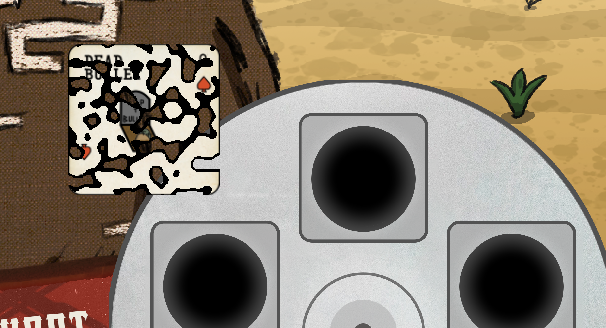
\includegraphics[width=0.6\textwidth]{card_destroy}
    \caption{Bild der Animation, wenn eine Karte zerstört wird}
\end{figure}

Um diesen Effekt zu erzeugen, wird dem Shader nicht nur die Kartentextur, sondern auch eine Noise-Textur mitgegeben.
Die Verwendung einer Noise-Textur statt im Shader generierten Noise hat den Vorteil, das sie deutlich performanter ist,
da die Noise-Werte im schon im Vorhinein berechnet sind.
Sonst müssten diese beim Rendern, im Shader, für jeden Pixel, berechnet werden.
Vorgefertigte Texturen haben allerdings den Nachteil, dass die Auflösung limitiert ist, und das die Noise-Parameter
zu Runtime nicht geändert werden können.

\begin{figure}[H]
    \centering
    
\includegraphics[width=0.3\textwidth]{perlin}
    \caption{Die verwendete Noise-Textur}
\end{figure}

Der Shader definiert zwei Thresholds, die mit der Noise-Textur abgeglichen werden.
Ab dem ersten Threshold wird statt der Kartentextur schwarz gerendert, ab dem zweiten transparent.
Ein stetiges Erhöhen der Thresholds erzeugt den Destroy-Effekt.

\subsubsection{Die Orb-Animation}

Die Orb-Animationen werden im Spiel verwendet, um zu signalisieren, wenn sich abstrakte Konzepte, die keine wirkliche
In-Game-Repräsentation hat, von einem Ort zu einem anderen bewegen.
Ein Beispiel dafür sind Reserves im Kampf oder das Cash am Ende des Kampfes.

\begin{figure}[H]
    \centering
    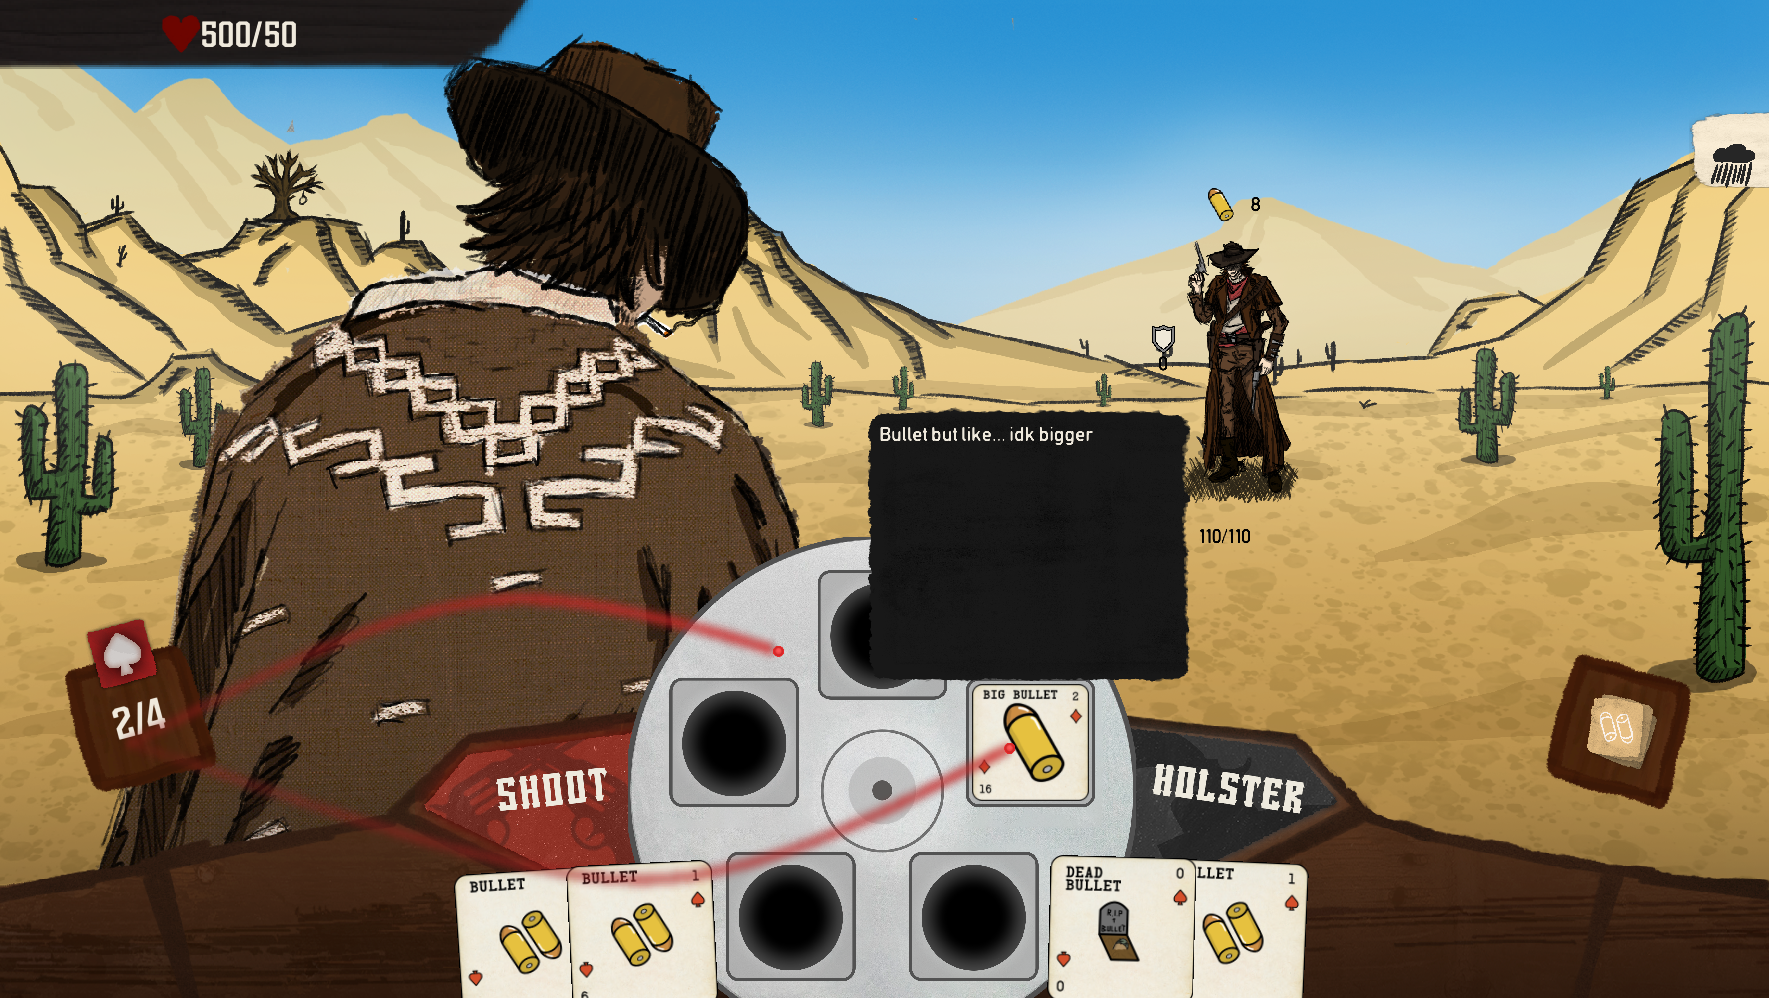
\includegraphics[width=1.0\textwidth]{orb_animation}
    \caption{Die Orb-Animation, wenn Reserves gezahlt wurden}
\end{figure}

Bei der Orb-Animation wird eine beliebige Texture von einem Ort zu einem anderen animiert, wobei sie dabei einen Schweif
hinterlässt.

Die Orb-Animation verwendet zwei Framebuffer, mit einer Ping-Pong-Strategie, wie im
Kapitel~\ref{subsubsec:postprocessing-effects} beschrieben.
Zusätzlich werden diese Framebuffer verwendet, um den Zustand des Schweifs über Frames hinweg zu speichern.
Das Rendern dieser Animation findet in zwei Stufen statt.
Zuerst wird der Framebuffer der Orb-Animation geupdated, danach wird die Animation auf den Bildschirm gerendert.
Der erste Schritt läuft folgendermaßen ab:

Zwei Framebuffer, hier A und B genannt, werden erschaffen, falls sie noch nicht existieren.
Beide Framebuffer haben nur die halbe Auflösung des Bildschirms, da das Renderzeit spart und durch den Blur-Effekt, der
im zweiten Schritt angewandt wird, nicht auffällt.
Zu Beginn enthält B den aktuellen Zustand des Schweifs.
Framebuffer B wird zu A gerendert, wobei ein spezieller Shader verwendet wird, der den Alpha-Kanal um einen festgelegten
Wert reduziert.
Bei dem Rendern des Framebuffers muss darauf geachtet werden, dass die OpenGL Blending Funktion richtig gesetzt ist,
um zu verhindern, dass der Inhalt der beiden Buffer anhand des Alpha-Werts geblendet wird.
Stattdessen soll der Farb-Wert des Shader-Outputs ohne Blending einfach übernommen werden.
Der Wert, um den der Alpha Kanal reduziert wird, wird mit der aktuellen Frametime multipliziert, um eventuelle
Lagspikes auszugleichen.
Diese Alpha-Reduktion wird durchgeführt, um dafür zu sorgen, dass der Schweif langsam ausbleicht.

Danach wird die Textur der Animation an der aktuellen Stelle zu Framebuffer A gerendert, um den Schweif um die passierte
Bewegung zu erweitern.
Optional kann die Textur auch mehrmals zwischen der letzten und der aktuellen Position gezeichnet werden, was vor allem
bei schnellen Animationen helfen kann, sichtbare Löcher im Schweif zu vermeiden.
Zum Schluss des ersten Schrittes werden die Framebuffer getauscht, was heißt, dass A zu B und B zu A wird.

Das Resultat dieses Schrittes ist der Framebuffer B, der in Abständen die Textur der Animation auf transparentem
Hintergrund enthält, wobei ältere Pixel einen niedrigeren Alpha-Wert haben.

\begin{figure}[H]
    \centering
    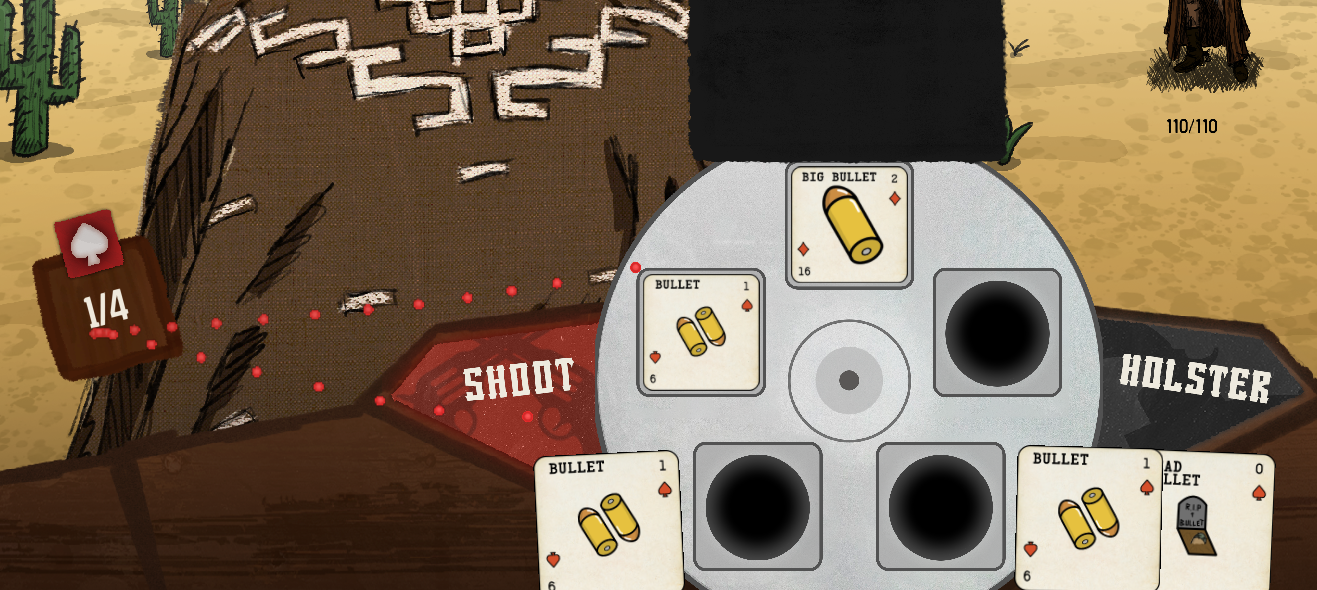
\includegraphics[width=1.0\textwidth]{orb_animation_fbo_B_low_segments}
    \caption{Inhalt des Framebuffer B, auf den Bildschirm gerendert, wobei eine Textur pro Frame gezeichnet wird }
\end{figure}

\begin{figure}[H]
    \centering
    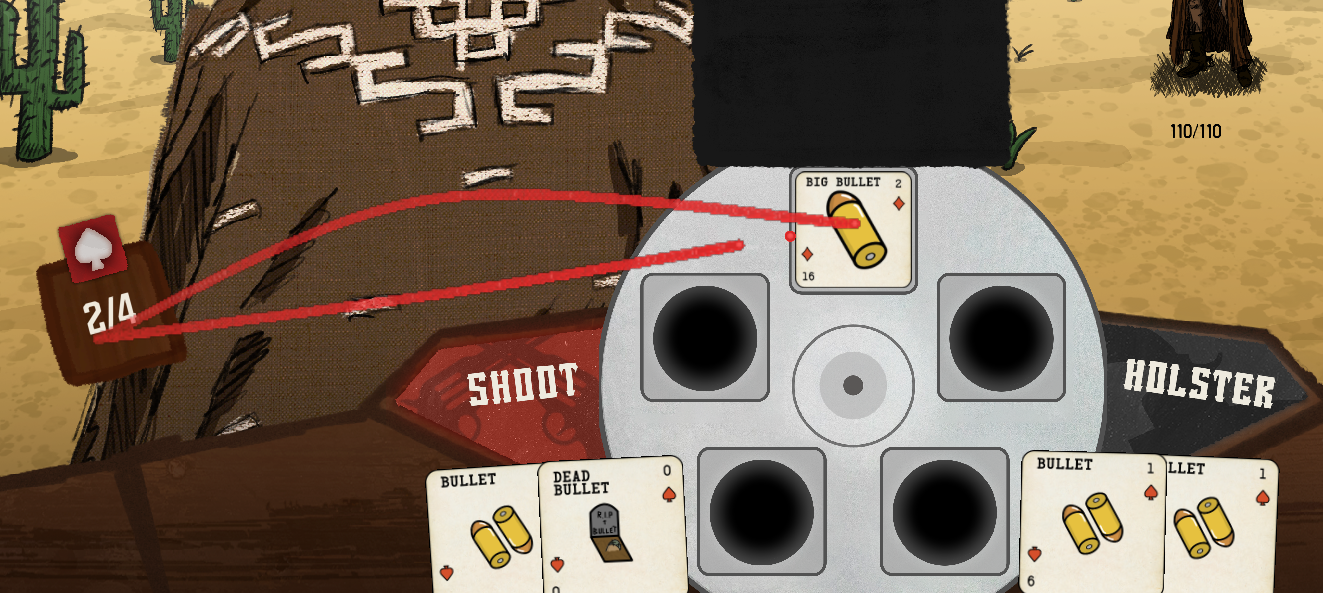
\includegraphics[width=1.0\textwidth]{orb_animation_fbo_B_high_segments}
    \caption{Inhalt des Framebuffer B, auf den Bildschirm gerendert, wobei 20 Texturen pro Frame gezeichnet werden }
\end{figure}

Im zweitem Schritt wird die Animation tatsächlich zum Bildschirm gerendert.
Dabei wird zuerst der Schweif aus Framebuffer B gerendert, und dann die Textur der Animation an der aktuellen Position.
Zweiteres ist trivial, der erste Teil aber nicht.
Bevor der Schweif gerendert wird, muss zuerst ein Blur-Effekt angewendet werden, damit die Texturen die zu Framebuffer
B gerendert wurden miteinander und mit dem Hintergrund verschwimmen.

Für die Orb-Animation wird ein 2-Pass Gaussian Blur verwendet, da dieser oft bessere Ergebnisse liefert als \zB ein
Box-Blur.\zit{gaussianBlur}
Allerdings ist ein Gaussian-Bur auch teurer zu berechnen, was aber unter anderem durch die halbierte Auflösung keine
Probleme macht.
Ein Blur-Effekt funktioniert, in dem für jeden Pixel die Textur nicht nur an der Stelle des Pixels gesampled wird,
sondern auch an umliegenden Stellen.
Die finale Farbe des Pixels ist dann der Schnitt aus all diesen Samples.
Was den Gaussian Blur von \ua einem Box-Blur unterscheidet ist, das die Samples anhand einer gaußschen Verteilung
gewichtet werden, was dazu führt, dass Pixel, die näher an der Mitte liegen, einen größeren Einfluss auf das Ergebnis
haben.\zit{gaussianBlur}
Diese Gewichte sind in einem Look-up-Table definiert, müssen also nicht jedes Mal berechnet werden.

Eine besondere Herausforderung bei dem Gaussian-Blur Shader war der Umgang mit Transparenzen.
Ein transparenter Pixel hat, auch wenn er nicht dargestellt wird, eine Farbe (Im Falle der Orb-Animation ist das Schwarz).
Wenn nun ein Pixel am Rand der Textur ist, wird auch im transparenten Bereich gesampled,
wo der Shader Schwarz zurückbekommt.
Das führt zu einer deutlichen Verdunkelung der Pixel am Rand des Schweifs.
Um dieses Problem zu lösen, wird das gaußsche Gewicht zuerst mit dem Alpha-Wert multipliziert, sodass transparente Pixel
keine/weniger Einfluss auf das Resultat haben.
Die tatsächlich verwendeten Gewichte werden gemeinsam mit den Samples aufsummiert und dann dividiert, um den Schnitt zu
erhalten.

Die Orb-Animation verwendet eine 2-Pass Version des Gaussian Blur, bei der zuerst horizontal, dann vertikal geblurred
wird.
Das heist aber auch, dass für den ersten Pass wieder zu einem Framebuffer gerendert werden muss.
Hier kann aber einfach Framebuffer A verwendet werden, da dieser zu diesem Zeitpunkt nicht in Verwendung ist.
Zum Schluss des zweiten Schritts wird die Textur der Animation ohne Blur direkt auf den Bildschirm gezeichnet.

% resets author
\renewcommand{\kapitelautor}{}




%
\chapter{Gamedesign}\label{ch:gamedesign}


\section{Einleitung}\label{sec:einleitung}

\renewcommand{\kapitelautor}{Autor: Philip Jankovic}


\FF ist ein digitales Kartenspiel in einem Wild West Setting. Der spieler reist durch den Wilden Westen auf einer Map,
sammelt Karten und bekämpft damit Gegner um auf der Map fortzuschreiten. Karten sind Bullets und werden in das Spielfeld, also den Revolver geladen.
Jede Bullet hat einen eigenen Effekt, der von dem Spieler genützt werden kann um immer bessere Combos aufzubauen und damit immer stärkere Gegner zu bekämpfen.
Der Revolver wird dazu verwedet, Bullets auf den Gegner abzufeuern. Nachdem eine Bullet geschossen wurde, verlässt die
Bullet den Revolver und der Revolver sich eines nach rechts. Der Gegner kann verschiedene Gegneraktionen ausführen und damit dem Spieler schaden.
Durch die  immer besser werdenden Bullets des Spielers, ist es ihm möglich, die immer schwerern Gegner zu bezwingen und damit den Wilden Westen zu durchqueren.
Die Map enthält verschiedene Biome und Events, durch die der Spieler neue Karten erwirbt oder er sich heilen kann.



\subsection{Begriffserklärung}\label{begriffserklärung}
Mechanik: In \FF sind Mechaniken einzelne Komponente des Spieles, welche zusammgesetzt das Spiel ergeben.

Combo: In \FF wird eine Combo als eine Kombination von Karten mit guter Synergie zueinander bezeichnet.


Map: Die Karte von \FF, auf der sich der Spieler bewegt und diverse Events auswählt, wie \zB Kämpfe oder Shops.

Road: Eine Road in \FF ist eine zufällig generierter Abschnitt des Spieles. Eine Road befinndet sich immer zwischen zwei Areas.

Area: Nicht zufällig gnerierte Abschnitte der \FF Map.

Rogue-Like: Ein Genre von Videospiel, bei welchem der Fortschritt des Spielers verloren geht, sollte er streben/verlieren.

Run: Ein Run ist ein Durchlauf in einem Rogue-like oder Rogue-lite Spiel. \zit{zitatdeckbuilding}

Rogue-Lite: Ein Subgenre des Rogue-Likes, bei welchem Teile des Fortschrittes in den nächsten Run mitgenommen werden.
Es ist einfacher und weniger frustrierend als ein Rogue-Like

% text goes here
%

% resets author
\renewcommand{\kapitelautor}{}


\section{Grundlegende Spielbestandteile}\label{sec:grundlegenste-regeln}

\renewcommand{\kapitelautor}{Autor: Philip Jankovic}


%
\FF ist ein digitales Kartenspiel im Subgenre des Rogue-lite Deckbuilders.
Der Spieler bewegt sich über eine Map, die prozentual generiert ist, sammelt Karten und benutzt diese Karten,
um Gegner zu bekämpfen. Sollte der Spieler einen Kampf verlieren, stirbt er, seine gesammelten Karten
gehen verloren und er startet wieder am Anfang. Da es sich jedoch um ein \quoted{Rogue-Lite} handelt und nicht um ein \quoted{Rogue-Like},
gibt es eine Art von speicherbarem Fortschritt, den der Spieler in sein nächstes Leben mitnehmen kann.
Ein Durchlauf bzw. ein Leben des Spielers wird als \quoted{Run} bezeichnet. Ein Run endet mit dem Tod des Spielers.
Während der Entwicklung wurden jene Elemente, die in das nächste Leben übergehen, als \quoted{Rogue-Lite-Elemente} bezeichnet.
\zit{roguelikedeckbuilder}



\begin{infoBox}
    Note: Zu diesem Zeitpunkt geht es nicht um die Designprinzipien hinter Bestandteilen,
    sondern nur um die Erklärung jener. Das Gamedesign wird in \ref{sec:Gamedesign} beschrieben.
\end{infoBox}


%zuerst erklären was roads und so sind????
\subsection{Rogue-Lite Elemente}\label{rogue_lite_elemente}

Da es sich bei \FF um ein \quoted{Rogue-lite} und kein \quoted{Rogue-like} handelt, hat der Spieler die Möglichkeit, gemachten Fortschritt mit in sein nächstes Leben zu nehmen.
Wie genau der mitgenommene Fortschritt ausschaut ist unterschiedlich von Spiel zu Spiel.\zit{roguelite}


Um das Spielerlebnis des Spielers nicht allzu frustrierend zu gestalten, wurden in \FF zwei verschiedene Mechaniken eingeführt.


Bei der ersten Mechanik handelt es sich um die Erhöhung der maximalen Lebenspunkte, manchmal auch HP-Wert genannt, des Spielers bei Heilpunkten im Spiel.
Der Spieler hat die Möglichkeit sich zu entscheiden, ob er sich lieber nur für diesen Run heilt und dafür auch eine größere Menge an Lebenspunkten erhält, oder ob er
lieber in das Erhöhen seiner Lebenspunktkapazität investiert. Bei letzterem handelt es sich natürlich um eine kleinere Zahl als bei der anderen Wahl.
Dies dient dazu, dem Spieler die Entscheidung offen zu halten, entweder etwas Langwieriges aber Bleibendes zu investieren oder lieber noch einmal ordentlich
Lebenspunkte aufzutanken, was bei der zweiten Mechanik ins Spiel kommt.

\begin{figure}[H]
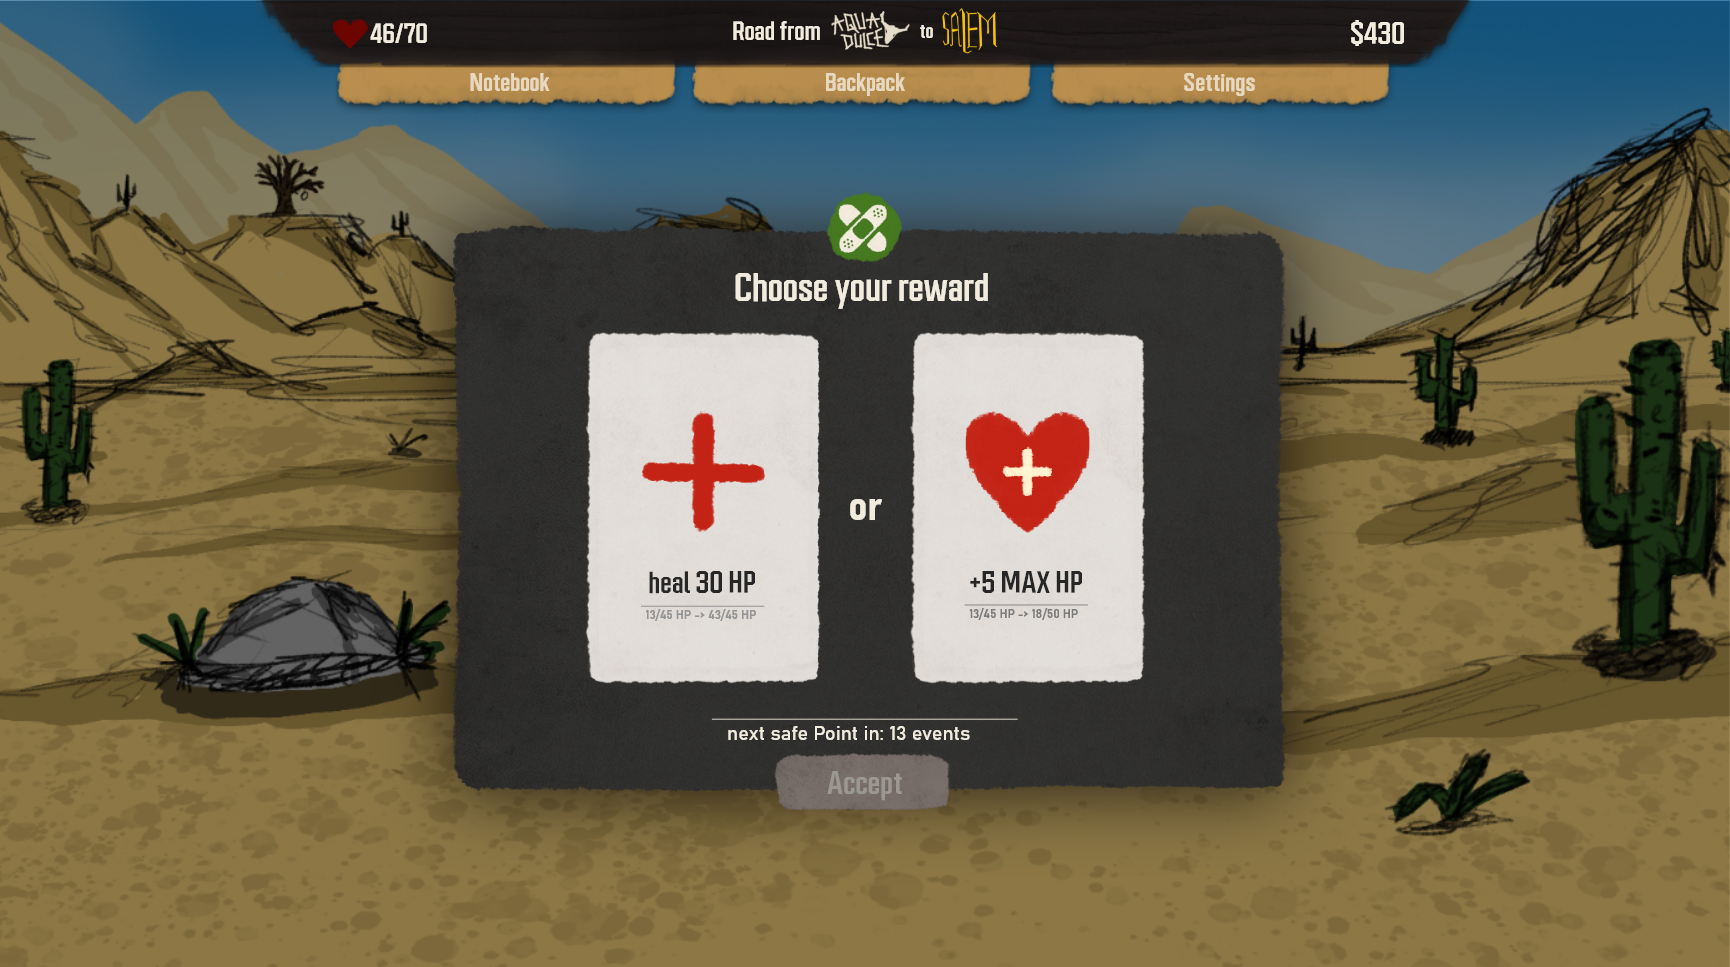
\includegraphics[width=\textwidth]{healeventgrafic.png}
\caption{Beispiel: Ein Heilevent}
\end{figure}


Die zweite Mechanik tritt in Kraft, sollte der Spieler  einen Abschnitt des Spiels, also eine sogenannte Road schaffen. Seine bis zu dem Zeitpunkt gesammelten Karten werden
gespeichert und sind ab dann selbst nach seinem Tod jederzeit zugänglich und spielbar.


Roads werden Abschnitte zwischen zwei Areas genannt und werden zufällig generiert. Areas werden nicht zufällig generiert.

\begin{figure}[H]
    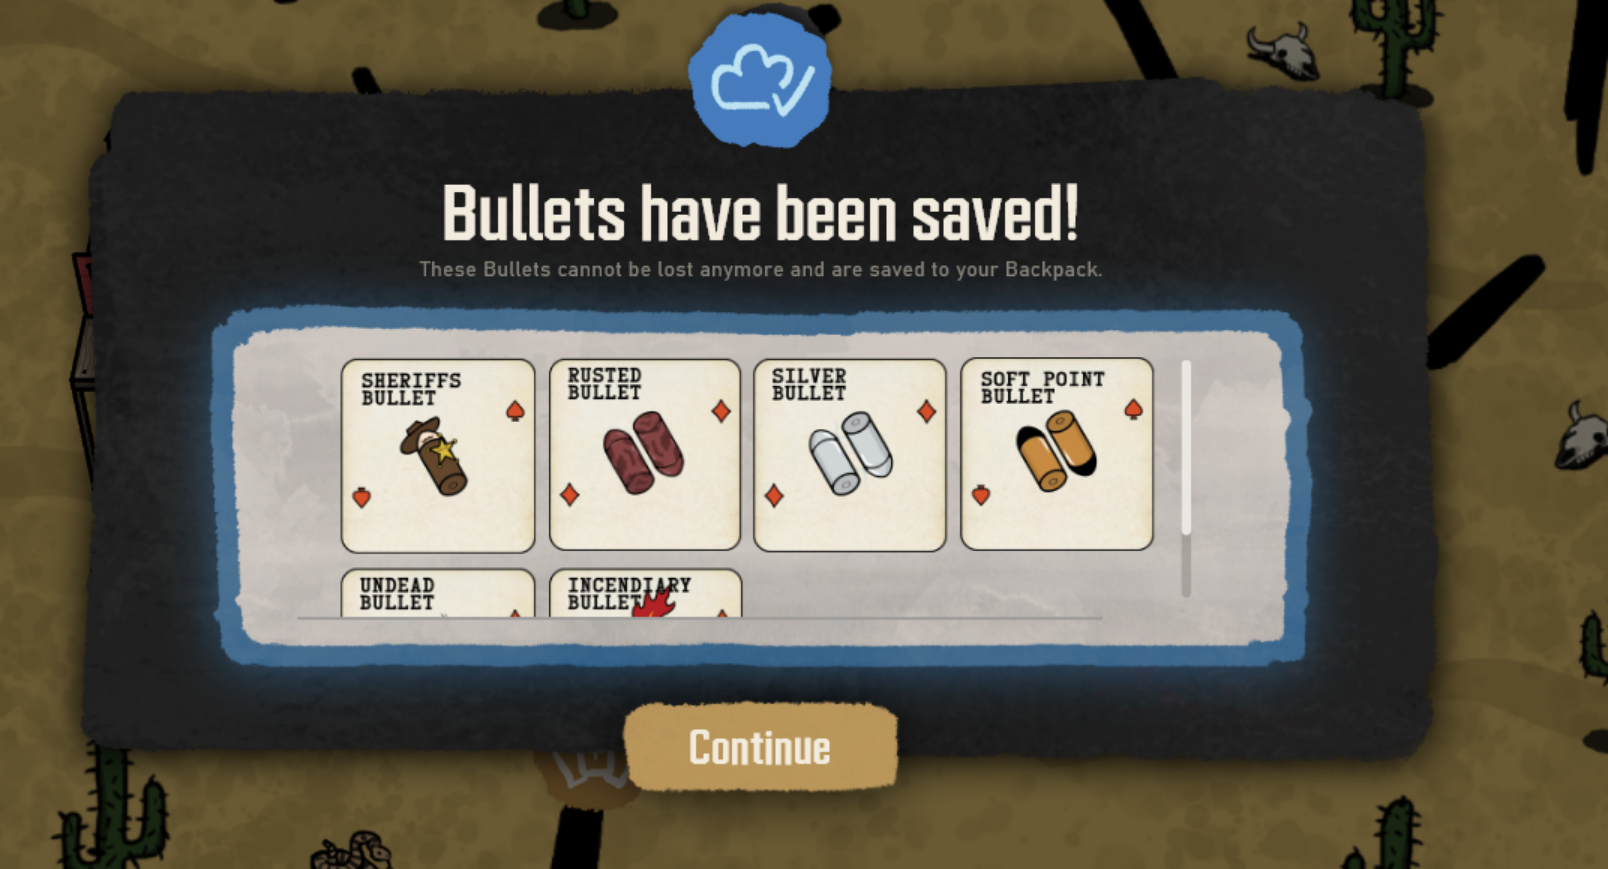
\includegraphics[width=\textwidth]{bulletssavedPopup.png}
    \caption{Beispiel: Das Popup, welches am Ende der Road erscheint um zu zeigen welche Karten gespeichert wurden.}
\end{figure}


\begin{figure}[H]
    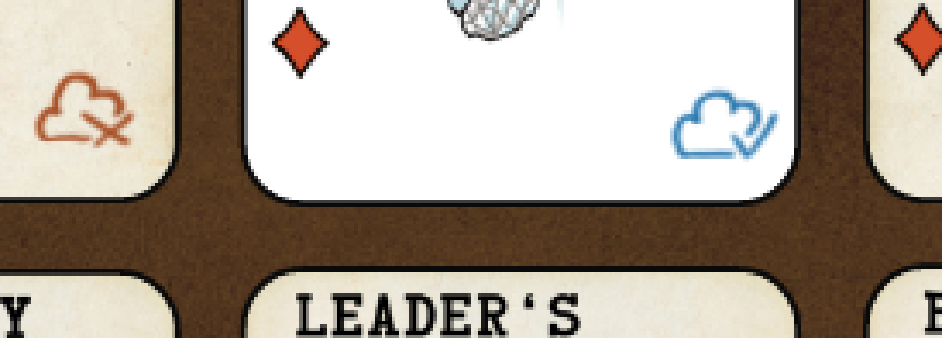
\includegraphics[width=\textwidth]{bulletsaved.png}
    \caption{Beispiel: Symbol einer bereits gespiecherten Karte}
\end{figure}

Verknüpft mit der ersten Mechanik
hat der Spieler die Möglichkeit, sich dazu zu entscheiden, seine Leben wieder aufzufüllen und das Ende der Road anzustreben.
Ist er der Meinung, es sowieso nicht mehr zu dem Abschnittsende zu schaffen, wählt er die Erhöhung der maximalen
Lebenspunkte, um so zumindest einen Vorteil in den nächsten Runs zu haben. Der Spieler muss also das Risiko und die
Belohnung abwägen und dann entscheiden, welche Wahl er trifft.



\subsection{Sammeln von Karten}\label{sammeln_der_Karten}

Nach jedem überlebten Kampf bekommt der Spieler eine neue Karte. Er bekommt drei verschiedene, zufällige Karten presentiert und darf sich eine davon auswählen.
Außerdem gibt es auf der Map verteilt noch zusätzliche Events, die der Spieler aufsuchen kann, um seine Sammlung zu erweitern.

\begin{figure}[H]
    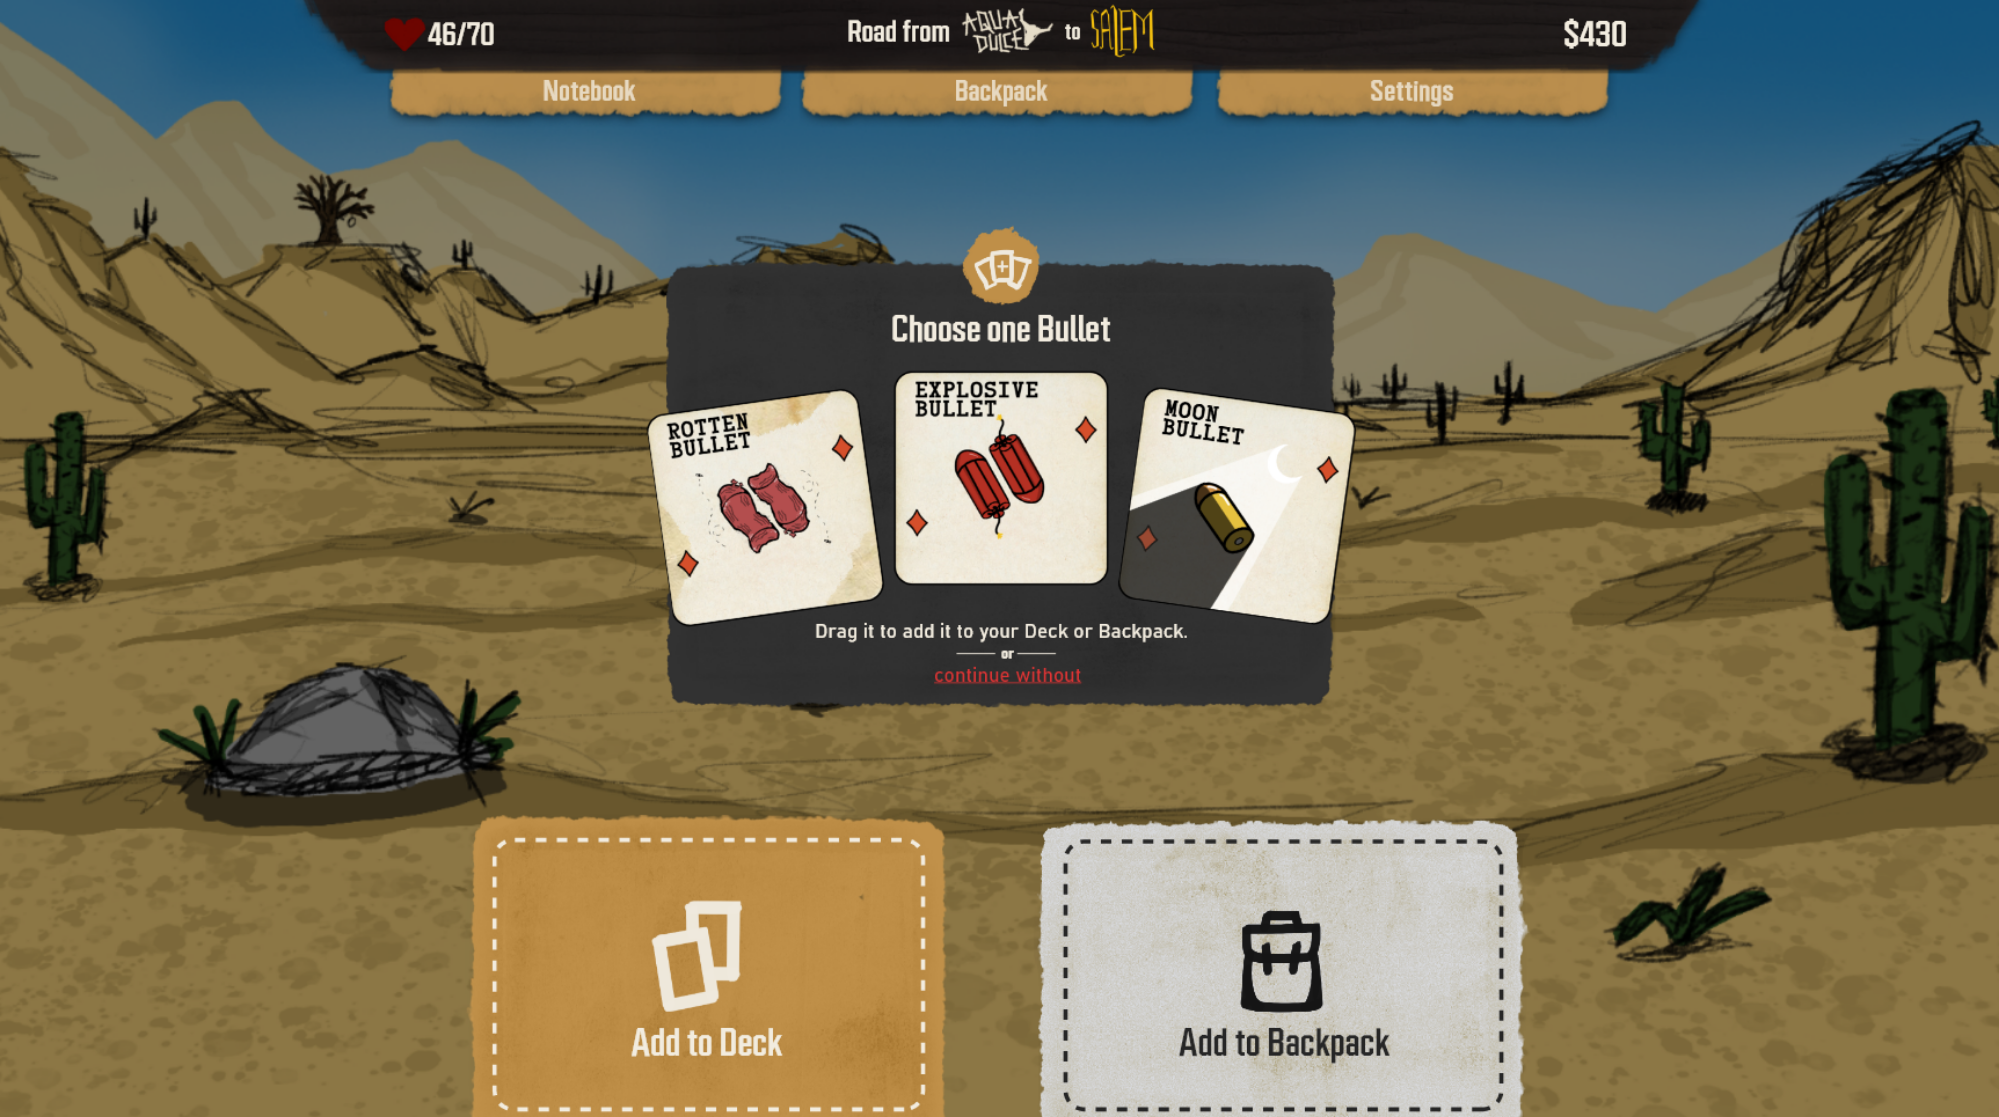
\includegraphics[width=\textwidth]{choosebullet.png}
    \caption{Beispiel: Popup, welches nach einem Kampf, oder auch auf der Map als Event erscheinen kann.}
\end{figure}

Das bringt nicht nur wieder eine Entscheidung des Spielers mit sich, die den Verlauf des Runs ändert, sondern bringt auch mehr Abwechslung,
da der Spieler nicht immer nur die Karten nehmen kann, die er gerne hätte. Es bringt auch eine Art Entdeckerlust mit sich, da der Spieler
auf diese Weise natürlich die Karten erst nach und nach sieht und nicht alle gleich auf einmal, anders als bei \zB \quoted{Magic Arena},
wo alle Karten sofort in einer eigenen Liste zugänglich sind. \zit{magicarena} Das zwingt den Spieler mit begrenzter Wahl an Ressourcen das Beste daraus zu machen.

"It is not that players build a deck in order to play the game, it is that they play the game in order to build a deck."\zit{zitatdeckbuilding}%TODO direkte zitate


Diese Designpolitik wird beim Design der Karten beachtet und es wird in dem Kapitel \ref{sec:Gamedesign} näher darauf eingegangen.


Viele Rogue-lite Deckbuilder haben ein ähnliches System. Inspiriert wurde das Sammeln der Karten in \FF von Spielen wie \quoted{Inscription} und \quoted{Slay the Spire},
es gibt jedoch einen großen Unterschied. Anders als in \zB \quoted{Slay the Spire} können Karten ganz einfach aus dem Kartendeck entfernt werden, nachdem sie einmal ausgewählt wurden.
Karten können aus dem Deck in den Backpack verschoben werden und ermöglichen dadurch ein flexibleres Spielerlebnis.\zit{slaythespire, inscryption, zitatdeckbuilding}


\begin{figure}[H]
    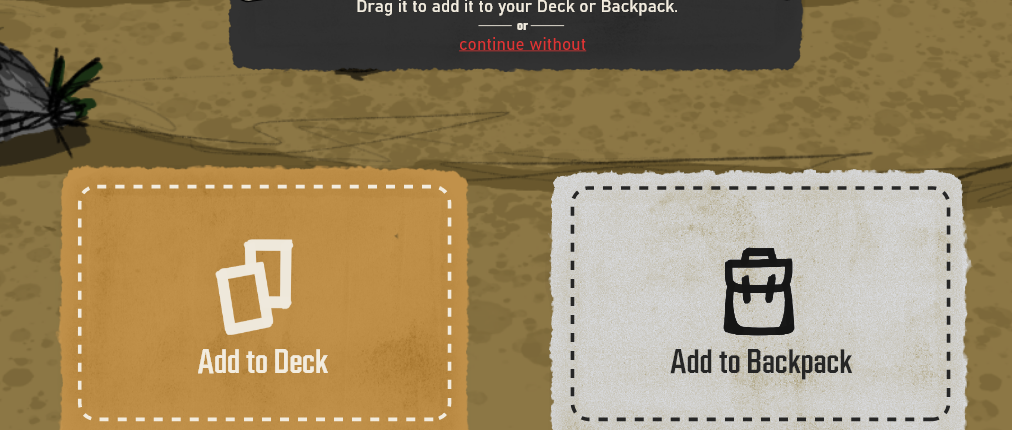
\includegraphics[width=\textwidth]{deckandbackpack.png}
    \caption{Beispiel: zwei Möglichkeiten, nachdem eine Karte ausgewählt wurde}
\end{figure}%

\subsection{Backpack und Deck}\label{backpack_and_deck}

Der Backpack und das Deck dienen beide als Speicherort für Karten, mit dem Unterschied, dass die Karten im Deck aktiv im
Kampf eingesetzt werden und die Karten im Backpack mehr als Reserve gelten.
Karten können frei zwischen den beiden verschoben werden, solange die festgelegte Mindestanzahl an Karten im Deck eingehalten wird.


Da \FF viele verschiedene Strategien bietet, gibt es mehrere Decks, zwischen denen der Spieler einfach wechseln kann.
Das hat zur Folge, dass der Spieler nicht immer ein Deck zerlegen muss, um eine andere Strategie auszutesten.

\begin{figure}[H]
    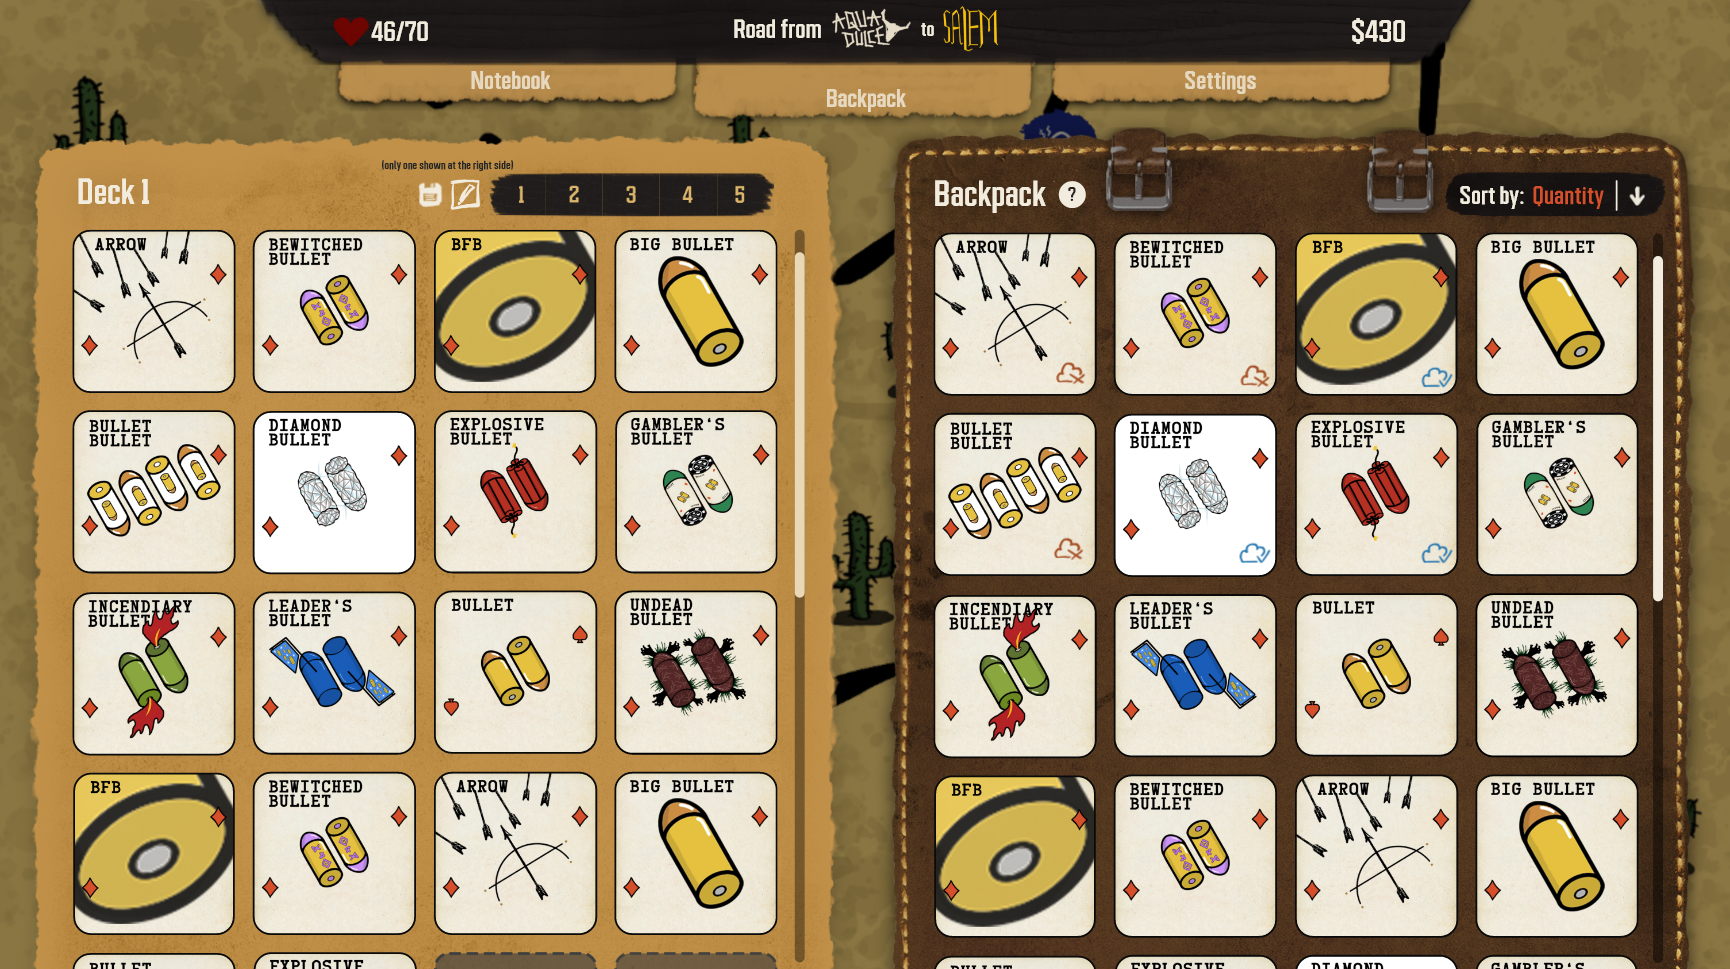
\includegraphics[width=\textwidth]{deckview.png}
    \caption{Beispiel: Ansicht eines Decks und des Backpacks}
\end{figure}

\begin{figure}[H]
    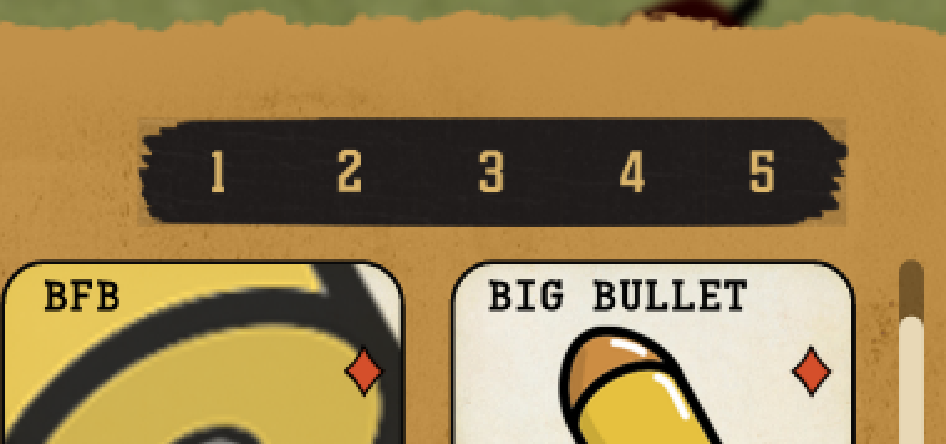
\includegraphics[width=\textwidth]{deckchoose.png}
    \caption{Beispiel: User Interface für das Wechseln des Deckes}
\end{figure}


Außerdem können Decks umbenannt werden, um besser wiedergefunden und erkannt zu werden.

Im Backpack können Karten nach Kriterien wie Kosten oder Namen auf- und absteigend sortiert werden.

\begin{figure}[H]
    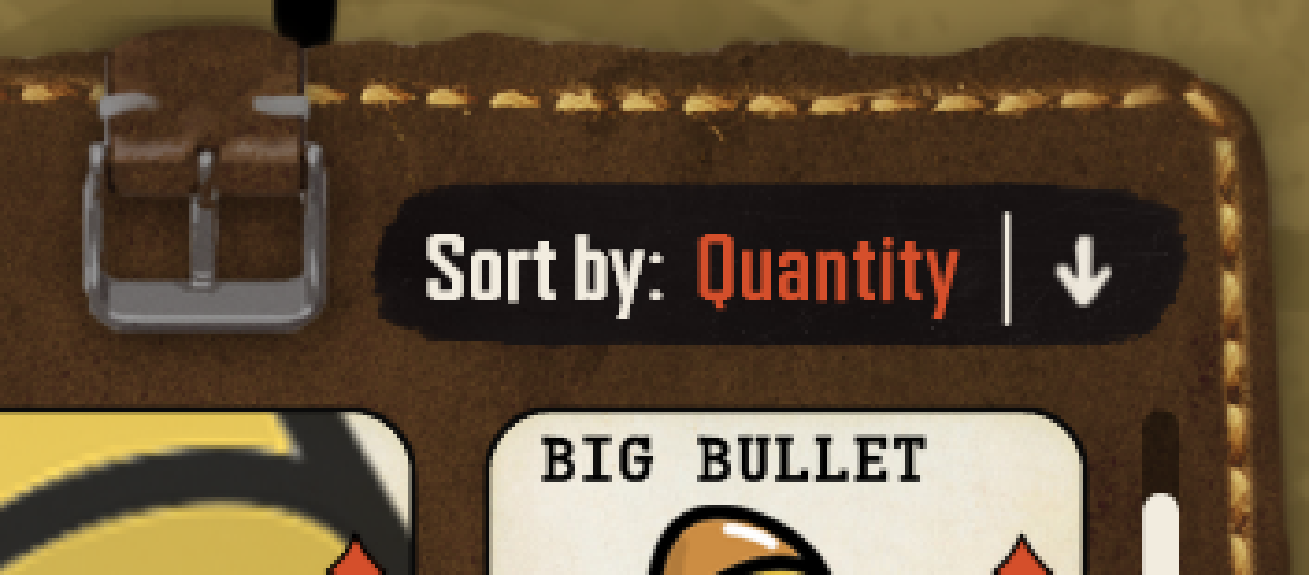
\includegraphics[width=\textwidth]{sortdeck.png}
    \caption{Durch Klicken kann durch verschiedene Sortierungs-Möglichkeiten durchgewechselt werden.}
\end{figure}

Sammelt der Spieler eine neue Karte, kann er sich entscheiden, ob er die Karte gleich seinem Deck oder doch eher seinem
Backpack hinzufügen möchte.
Der Backpack und das Deck ermöglichen es dem Spieler, Karten, die er gesammelt hat, aus dem Deck zu nehmen und damit
nicht zu verwenden, sowie Decks zu bauen, die zu einer Strategie passen.
Startet der Spieler nun einen Kampf, wird das zuletzt ausgewählte Deck verwendet.


\subsection{Kampf}\label{backpack_and_deck}
%grundsätzliche sachen wie reserves, gegner und spieler, gewonnen wenn gegner tod usw karten am anfang ziehe zwei karten am anfang vom turn

Während der Spieler über die Map reist, sind Kämpfe unausweichlich.


Kämpfe werden auf der Map durch zwei gekreuzte Revolver dargestellt. Um weiter auf der Map fortzuschreiten müssen sie absolviert werden.

\begin{figure}[H]
    \centering
    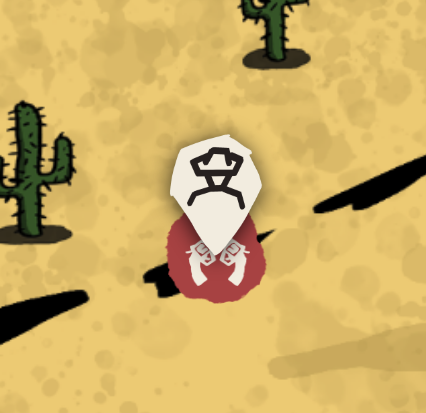
\includegraphics[width=0.5\textwidth]{playericon.png}
    \caption{Beispiel: Eventsymbol für einen Kampf}
\end{figure}

Gekämpft wird mit den gesammelten Karten, mit dem Ziel, den oder die Gegner zu besiegen und dabei so wenig Lebenspunkte
wie möglich zu verlieren \bzw nicht zu sterben.

Gewonnen hat der Spieler, wenn alle Gegner besiegt wurden.


Ein Kampf ist aufgeteilt in Züge. Immer abwechselnd ist entweder der Spieler oder der Gegner dran. Am Anfang des Kampfes
werden eine vordefinierte Anzahl an Karten vom Deck des Spielers gezogen.
Anschließend hat der Spieler die Möglichkeit, nach Belieben seinen Zug auszuführen. Ein Spielerzug wird mit dem \quoted{Holster}
Button beendet, und das Betätigen des Knopfes startet den automatischen Ablauf des Gegnerzuges. Der Gegner führt eine -mehr
oder weniger- zufällige Aktion aus, und danach ist wieder der Zug des Spielers.


Am Start des Zuges des Spielers werden zwei Karten vom Deck gezogen. Pro Zug stehen dem Spieler vier \quoted{Reserves}
zur Verfügung. Diese werden jeweils auch am Anfang des Zuges wieder auf die maximale Anzahl aufgefüllt.
Reserves können dazu verwendet werden, Karten zu bezahlen und damit auch zu spielen.

\begin{figure}[H]
    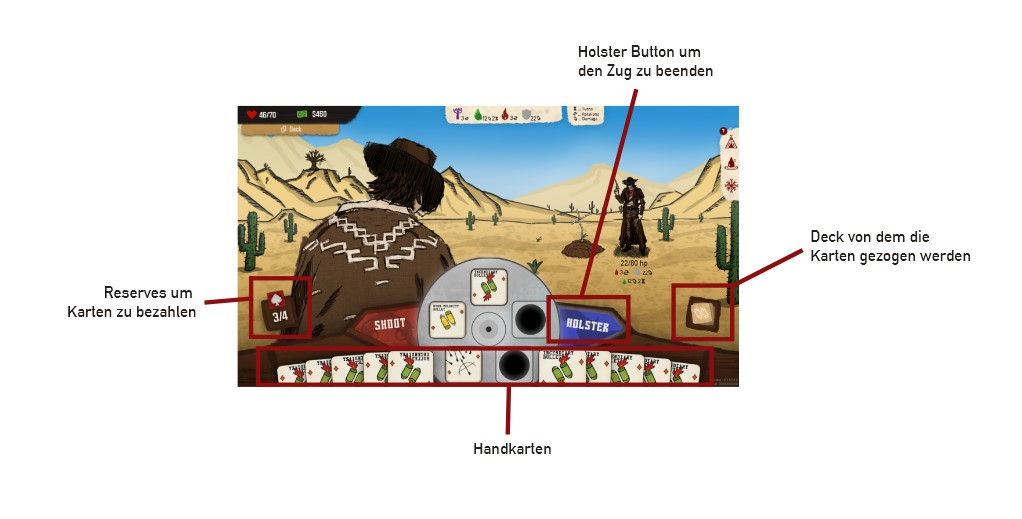
\includegraphics[width=\textwidth]{turngrafic.jpg}
    \caption{Beispiel: Kampf User-Interface in welchem alle benötigten Infos dargestellt werden.}
\end{figure}



\subsection{Karten}\label{Karten}
Karten in \FF sind Bullets. Jede Bullet hat einen Kosten-Wert, der mit \quoted{Reserves} bezahlt werden muss, um die Karte zu spielen, also zu benützen.
Die \quoted{Reserves}, die für die Bullet benötigt werden, werden automatisch bezahlt, falls der Spieler sich die Bullet leisten kann.
Ein gutes Management der Reserves und die Reihenfolge, in der man die Karten spielt, ist wichtig, um das Spiel zu meistern.


Jede Bullet hat außerdem einen Damage-Wert, auch Schadens-Wert, Dmg-Value oder Dmg-Wert genannt, welcher angibt, wie viele Lebenspunkte dem Gegner
durch die Karte abgezogen werden, falls die Karte auf den Gegner geschossen wird.

\begin{figure}[H]
    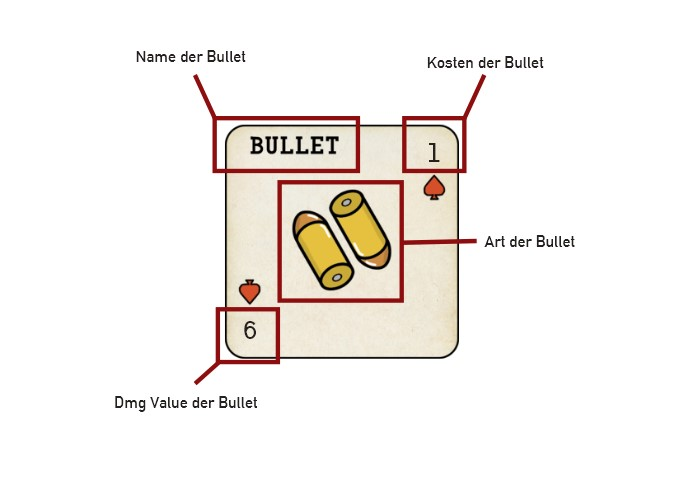
\includegraphics[width=\textwidth]{bulletgrafic.jpg}
    \caption{Beispiel: Die wichtigsten Infos werden auf der Karte angezeigt.}
\end{figure}

Fast alle Karten haben außerdem einen einzigartigen Effekt,
welcher angesehen werden kann, indem der Spieler mit der Maus über die gewünschte Bullet hovert.
In dem Popup, welches nach dem Hovern sichtbar ist, befinden sich die Infos zu dem Effekt der Karte.
Dazu gehört fast immer ein Trigger und der Effekt selbst.


Der Trigger gibt an, wann sich der Effekt aktiviert.


\begin{figure}[H]
    \centering
    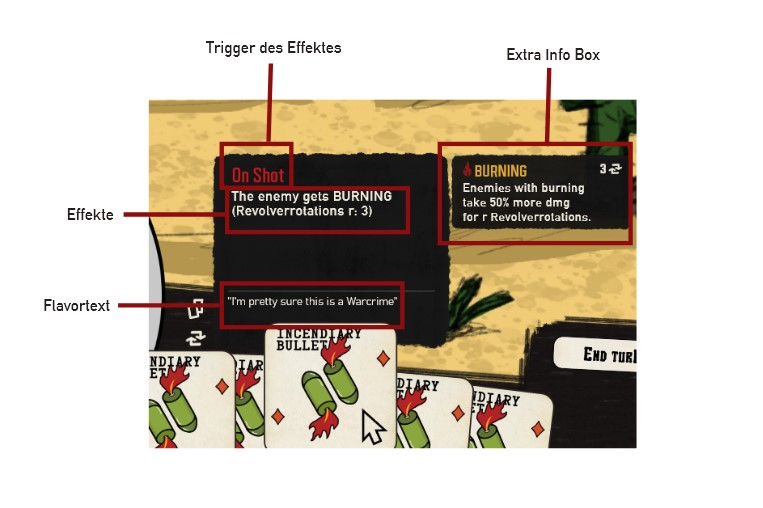
\includegraphics[width=0.5\textwidth]{hovergrafic.jpg}
    \caption{Beispiel: Hoverdetails,welche Infos über die karte zeigen}
\end{figure}



Es gibt verschiedene Trigger, wie \zB das Aktivieren des Effektes beim Spielen der Bullet.


Zusätzlich zu dem Effekt und dem Trigger steht bei vielen Karten außerdem noch ein Flavortext.
Ein Flavortext ist ein Spruch, der der Bullet ein wenig Kontext hinzufügt.
Es kann sich um einen Spruch, einen Witz, eine Anspielung oder einen story- \bzw worldbuilding-relevanten Text handeln.


Falls nötig werden relevante Infos zu dem Effekt in einer extra Box rechts oder links angezeigt.


Bullets werden, wenn sie gespielt werden, in den Revolver geladen.


\subsection{Revolver}\label{der_revolver}

Der Revolver ist das Spielfeld von \FF, in welches die Bullets platziert \bzw \quoted{geladen} werden.
Mithilfe von \quoted{Drag and Drop} kann der Spieler die Karte aus seiner Hand in den Revolver legen, diese Aktion des Ladens wird auch als Spielen der Bullet bezeichnet.
Im Zug des Vorganges werden Reserves in Höhe des Kosten-Wertes der Bullet abgezogen.


Der Revolver besteht aus fünf Kammern bzw. Feldern, in die Bullets geladen werden können.
Sie sind intern von eins bis fünf nummeriert.


Der Revolver kann von dem Spieler abgefeuert werden. Wenn geschossen wird, wird die Bullet in der obersten Kammer auf den Gegner geschossen.
Verlässt sie den Revolver, verliert der Gegner Lebenspunkte in Höhe des Damage-Wertes der geschossenen Bullet.
Die Bullet wird unter das Deck gelegt und der Revolver dreht sich einmal nach rechts.

\begin{figure}[H]
    \centering
    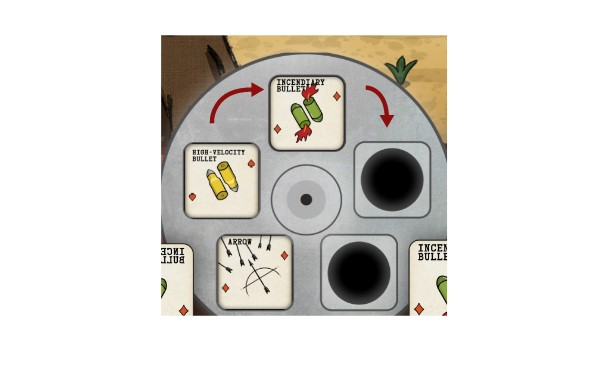
\includegraphics[width=\textwidth]{rotategrafic.jpg}
    \caption{Beispiel: Revolverdrehung nach rechts}
\end{figure}


Die Revolverrotation ist ein wichtiger Teil von \FF, da der Spieler sich das Placement der Bullets im Revolver genau überlegen muss,
um das Meiste aus seinen Bullets herauszuholen.


Weiters gibt es Karten mit Effekten, die sich auf die Revolverrotation auswirken, wie \zB \quoted{Bewitched Bullet},
welche den Revolver nach links statt nach rechts rotiert.


Die Komplexität von \FF kommt vom Meistern des Revolvers, der strategischen Platzierung und Reihenfolge der Bullets und dem Verstehen,
wie eine Revolverrotation sich auf die Bullets, den Spieler oder den Gegner auswirkt.


Die \quoted{Bewitched Bullet} kann \zB dazu verwendet werden, Karten,
welche davon profitieren, lange im Revolver zu bleiben, länger vom Abschuss zu bewahren. \quoted{Bull et} zum Beispiel fügt dem Gegner Schaden zu,
wenn sie im Revolver rotiert und profitiert damit von der Linksdrehung von Bewitched Bullet.


\begin{figure}[H]
    \centering
    
\includegraphics[width=0.3\textwidth]{bewitched_Bullet.png}
    \caption{Beispiel: Bewitched Bullet}
\end{figure}

\begin{figure}[H]
    \centering
    
\includegraphics[width=0.3\textwidth]{bull_et.png}
    \caption{Beispiel: Bull et Bullet}
\end{figure}


\subsection{Gegner}\label{gegner}
Der Gegner, auf den die Bullets des Spielers geschossen werden, besteht aus mehreren Komponenten.
Genau wie der Spieler verfügt der Gegner über einen HP-Wert. Wenn der Wert null erreicht, stirbt der Gegner.


Während dem Zug des Spielers zeigt der Gegner die Aktion an, die er in seinem nächsten Zug ausführen wird.
Nachdem der Spieler \quoted{Holster} gedrückt hat, beendet er seinen Zug und der Gegner ist dran.

Gegneraktionen werden zufällig ausgewählt aus dem Pool von Aktionen.
Jedoch wurden die Aktionen angepasst, um nicht nur Fairness zu garantieren,
sondern auch eine Balance zwischen mehr oder weniger anspruchsvoll zu finden.
Mehr zum Balancen der Gegner kann im Kapitel \ref{sec:Gamedesign} nachgelesen werden.


Sobald der Gegner am Zug ist, wird die Aktion automatisch ausgeführt. Je nach Gegnertyp gibt es andere Aktionen,
die ein Gegner ausführen kann. Universell ist jedoch die Aktion des Schaden zufügens.
Es gibt viele verschiedene Arten von Gegneraktionen, die dafür entwickelt wurden, mehr Abwechslung beim Bekämpfen der Gegner zu bieten.

Das Gegnerverhalten ist entstanden durch das Beobachten von Spielen im selben Genre, wie zum Beispiel \quoted{Slay the Spire}. \zit{slaythespire}


Außerdem sollte noch erwähnt werden, dass es auch passieren kann, dass der Spieler gegen mehr als einen Gegner kämpft.
Ist das der Fall, markiert der Spieler sein Ziel, indem er auf den gewünschten Gegner klickt.



Die geplannten Aktionen der Gegner sind durch Symbole über ihren Köpfen dargestellt. Der spieler hat die Aufgabe,
diese Aktionen in die Plannung seines Zuges miteinzubeziehen. Eine mögliche Reaktion auf das Zufügen von Schaden ist das parrieren.


\subsection{Parrying}\label{parrying}
Das parieren des Schadens, der vom Gegner verursacht wird, wird in \FF durch Bullets erreicht.


Der Spieler bekommt die Wahl, ob er parieren möchte oder nicht, was durch ein eigenes Popup während des gegnerischen Zuges geregelt wird.
Entscheidet sich der Spieler dazu zu parieren, wird dafür die Bullet im vordersten Slot verwendet.
Dann wird der Schadenswert des Gegners mit dem der Bullet gegengerechnet. Ist der Schadenswert der Bullet größer als der des Gegners,
geht kein Schaden durch. Ist es andersrum, bekommt der Spieler so viel Schaden zugefügt wie die Differenz ausmacht.


Es ist wichtig zu erwähnen, dass nicht pariert werden muss, wenn der Spieler die Bullet lieber behalten will, und den Schaden einfach einzustecken kann.
Durch einen Parry verlässt die Bullet den revolver und sie wird danach wieder unters Deck gelegt.


\subsection{Spezifische Regeln}\label{spezifische_regeln}

Es gibt einige zusätzliche spezifische Regeln in \FF. Beispielhaft werden folgende zwei erläutert.

\subsection{Overkillschaden}\label{Overkill}

Die erste ist der sogenannte Overkillschaden.
Die Regel besagt, dass jeglicher Schaden, der dem Gegner zugefügt wird, nachdem seine Lebenspunkte bereits unter 0 sind,
in Geld umgewandelt wird. Das Geld kann benutzt werden, um sich bei einem Shop weitere Karten zu kaufen.
Die Overkill-Regel gilt jedoch nur für den aktuellen Zug. Drückt der Spieler auf \quoted{Holster}, wird der Zug und der Kampf beendet.


Overkill-Cash, das durch Overkillschaden verdiente Geld, ist nicht nur eine gute Möglichkeit, Belohnungen anhand der Leistung des Spielers zu berechnen.


sondern löst auch gleichzeitig folgendes Problem: In \FF ist der Aufbau des Revolvers und damit von Combos sehr wichtig.
Oft kommt es vor, dass der Spieler eine Combo aufgebaut hat, der Gegner jedoch einfach schneller tot ist.
Das ist nicht nur frustrierend, sondern gibt dem Spieler auch einfach keinen Grund, überhaupt starke Combos aufzubauen,
wenn er sich einmal über dem Standard-Gegner-Schwierigkeitslevel befindet. Overkill-Schaden löst diese beiden Probleme.


\subsection{Leerschüsse}\label{leerschüsse}

Die zweite Regel bezieht sich auf das Schießen des Revolvers.
Die Regel besagt, dass, wenn der Revolver leer geschossen wird, also keine Bullet in der vordersten Kammer vorhanden ist,
der Spieler 5 Lebenspunkte Schaden erleidet.

Die örtliche Platzierung, der Zeitpunkt und die reihenfolge ist das wichtigste beim Platzieren der Bullets.

Einen Bullet in den hintersten oder ersten Slot zu platzieren, ist eine Entscheidung, die überlegt sein sollte.
Ohne die Leerschuss-regel ist es jedoch möglich, Bullets, die man weiter hinten platziert hat, sofort wieder vorrotieren zu lassen,
was das gesamte Spielprinzip der Revolverrotation ruinieren würde, da das Platzieren keine Konsequenzen hätte.
Es würde dazu führen, dass Bullets nacheinander einfach in den Revolver geladen werden, wo es gerade passt, und sofort
geschossen werden, da die Schussreihenfolge der Bullets ja sowieso egal ist.


Jedoch wollten die Entwickler das Rotieren des Revolvers ohne eine Bullet in dem vordersten Slot durch das Schießen nicht verbieten, sondern führten ein,
dass 5 Lebenspunkte abgezogen werden. Das bedeutet also, dass es im Notfall gemacht werden kann, z.B. falls es einmal für
eine Combo nötig ist, jedoch nicht durchgehend benutzt werden kann, da der Spieler durch das Abziehen der Lebenspunkte sonst stirbt.
Es ist eigentlich ein perfektes Beispiel, wie man durch das nicht direkte Verbieten einer Mechanik die Komplexität und
Möglichkeitsvielfalt wachsen lassen kann.


\subsection{Encounter Modifier}\label{encounter_modifier}


Encounter Modifier sind extra Regeln, die einem Kampf hinzugefügt werden um noch mehr Abwechslung in das Spiel zu bringen
und um den Spieler auch manchmal zum Wechseln der Kartenstrategien zu bringen.
Sie sind vor dem Kampf einsehbar, um das Umbauen oder Wechseln eines Decks noch zu ermöglichen.
Encounter Modifier können ganz verschieden sein.

Es gibt verschiedene Arten von Modifiern, einige untertützen, andere Schaden dem Spieler. Andere wiederum stellen die Regeln von \FF auf den Kopf.
Der Encounter Modifier \quoted{Frost} zum Beispiel friert den Revolver ein, was die Auswirkung hat, dass sich der Revolver  nach einem Schuss nicht mehr dreht.
\quoted{Bewitched Mist} lässt den Revolver immer statt nach rechts nach links drehen, was natürlich auch sehr verwirrend sein kann.

% resets author
\renewcommand{\kapitelautor}{}


\section{Flavor}\label{sec:flavor}

\renewcommand{\kapitelautor}{Autor: Philip Jankovic}

\subsection{Definition Falvor}\label{subsec:wichtigkeit-des-flavours}
%
Mit Flavor, im Bezug auf Kartenspiele, ist gemeint, welche Geschichten und Hintergründe hinter den einzelnen Karten stecken.
Es verknüpft die Optik, den Namen und die Funktion mit der Idee bzw dem Konzept der Karte.
Flavor gibt jeder Karte etwas Eigenes, was sie von anderen unterscheidet.

\begin{coolQuote}
    Flavor is the Soul of the game
\end{coolQuote}
\zid{soulOfTheGame}

Flavor kann auf verschiedene Arten auftreten. Flavor kann in Karten und generell in Spielkonzepten/Regeln existieren.
Es verknüpft die Karten, das Setting, die Story und die Spielregeln. Grob kann ein Kartenspiel in Funktion und Flavor aufgeteilt werden.
Beide existieren zusammen und keines ist wichtiger als das andere.
Unter Funktion wird verstanden, wie das Spiel gespielt wird, was Regeln und Mechaniken einschließt.\zit{flavorAndFunction}


\subsection{Flavor durch Spielmechaniken und Spielmechaniken durch Flavor}

Flavor und Funktion, zusammen also Spielmechaniken, sind das Erste, über das nachgedacht werden sollte wenn man ein Kartenspiel designed.
Flavor in den Spielregeln erlaubt Spielern, bereits vorhandenes Wissen im Spiel anzuwenden und das Spiel dadurch besser zu verstehen. \zit{flavorAndFunction}


In \FF ist das Spielfeld der Revolver. Vielen Spielern ist bereits bewusst, dass Bullets in einen
Revolver geladen werden. Da alle Karten Bullets sind, kann sich der Spieler denken, das die Karten in den Revolver geladen werden. Die Mechanik des Ladens
der Karten in das runde Spielfeld greift in den Flavor, der besagt, dass diese Karten Bullets sind und das runde Spielfeld
ein Revolver ist. Wären die Karten keine Bullets, sondern zum Beispiel Kreaturen und der Revolver kein runder Kreis,
der rotieren kann, wäre \FF nicht \FF, sondern ein anderes Spiel mit dementsprechend anderem Setting, kein Wild-West
Spiel und würde dementsprechend mit einem anderen Flavor verbunden sein.


Die Trommelrotation und das Abschießen von Bullets macht nur Sinn, da das Spielfeld ein Revolver ist.
Dass die Karten Bullets sind, macht nur Sinn, weil das Setting im Wilden Westen spielt und das Spielfeld ein Revolver ist.
Dass das Spielfeld ein Revolver ist, macht nur Sinn, da er nach rechts rotiert und die vorderste Karte rausschießt wenn er abgefeuert wird.
Ohne den Flavor sind die Spielregeln von \FF unnachvollziehbar und können ohne das andere nicht exestieren.


Anders gesagt, gibt der Flavor einem Kartenspiel, welches eigentlich nur ein abstraktes Konzept aus Nummern und Regeln ist,
an welche sich Menschen halten, damit ein Spiel zustande kommt, einen Grund für die Funktionalitäten und damit eine \quoted{Seele}.


Auch in \quoted{Magic the Gathering}, \quoted{Inscription} oder \quoted{Balatro} ist dieses Konzept sichtbar.

In \quoted{Magic the Gathering}
ist das Spielkonzept breit und umfangreich.
Das Setting ist nicht so streng definiert wie in \FF, was mehr verschiedene Spielmechaniken und Karten ermöglicht.
Dafür fühlt sich das Spiel manchmal nicht mehr an wie \quoted{Magic the Gathering},
was bei \FF durch die strikte Einhaltung der Mechaniken und der Karten, also Bullets und dem Revolver, nicht passieren kann.\zit{magicarena}


Der Flavor von \FF ist stark und das durchziehende Konzept der Bullets so konstant, dass das Spiel und seine Regeln immer
wiederzuerkennen sind. Ähnlich ist es bei \quoted{Balatro}, einem pokerinspirierten Rogue-lite Deckbuilding Spiel.
So wie die sammelbaren Karten in \FF Bullets sind, sammelt der Spieler in \quoted{Balatro} verschiedene Joker Karten.
Obwohl \quoted{Balatro} erst veröffentlicht wurde, als die erste Release-Version von \FF die Entwicklung bereits abgeschlossen hatte,
ist das Konzept von den verschiedenen und komischen Jokern von \quoted{Balatro} sehr ähnlich zu den verschiedenen und
komischen Bullets von \FF. \zit{balatro}


\quoted{Inscription} wiederum verfügt über weniger konstantes Kartendesign, auch wenn jede Karte ein anderes Tier darstellt,
legt dafür aber Wichtigkeit auf das Setting und die Stimmung, die das Spiel vermittelt. Durch Opfern von Karten können stärkere Karten
gespielt werden, was gut zu dem Horrorsetting passt. Auch Lebenspunkte werden abgerechnet durch herausgerissene Zähne und Augen.\zit{inscryption}


All diese Beispiele zeigen, wie Spiele aus demselben oder sehr ähnlichen Genre sich durch ihr Setting, Flavor und Spielmechaniken unterscheiden.


\begin{figure}[H]
    \centering
    
\includegraphics[width=0.5\textwidth]{4games.png}
    \caption{Beispiel: vier verschiedene Deckbuilding Spiele}
\end{figure}


Die Erschaffung der Spielregeln und damit auch des Flavors von \FF gingen Hand in Hand miteinander.
Zuerst kam die Idee des Settings des Wilden Westens, dann das Spielkonzept. Mehr zu Methoden kann in \ref{sec:methoden}
nachgelesen werden. Wichtig für dieses Kapitel ist, dass selbst nach zwei Jahren Arbeit und vielen Änderungen an Spielregeln,
das Grundkonzept noch immer das gleiche ist. Viele Karten, die zu Beginn der Entwicklung in Notizbüchern aufgezeichnet wurden, befinden sich
fast identisch noch immer im Spiel.



Spielmechaniken sind jedoch nicht das Einzige, in dem Flavor eine wichtige Rolle spielt.

\subsection{Cardflavor}\label{subsec:cardflavor}

Cardflavor ist der Flavor einzelner Karten.
Dazu gehört ihr Name, ihre Optik, ihr Effekt, wie der Effekt mit dem Namen der Karte zusammenhängt,
ihr Platz in der Welt und ihre Hintergrundgeschichte. Je nach Karte sind mehr oder weniger der genannten
Merkmale vertreten.


Zusätzlich zu dem Effekt der Karte, der sichtbar wird, wenn der Spieler über die Karte hovert, haben einige Karten zusätzlich einen sogenannten Flavortext.
Flavortexte sind zum Beispiel auch in \quoted{Magic the Gathering} vertreten und beschreiben die Welt der Spieles oder geben
Zitate von verschiedenen Charakteren in der Magic-Welt wieder.\zit{magicarena,soulOfTheGame}


Auf den Bullets von \FF kann ein Flavortext entweder Worldbuilding, ein Spruch, ein Witz oder eine Anspielung sein, die zur Karte passt.


\begin{figure}[H]
    \centering
    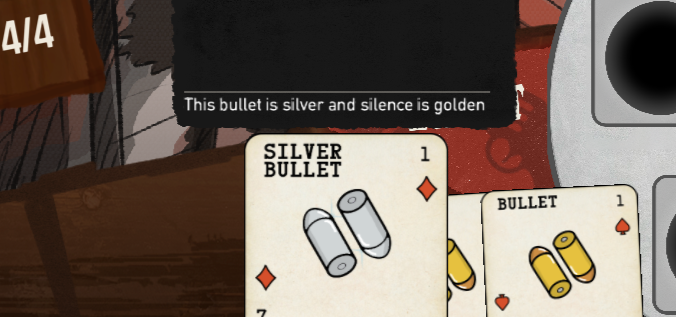
\includegraphics[width=0.5\textwidth]{flavorscreen.png}
    \caption{Beispiel: Flavortext von \quoted{Silver Bullet}}
\end{figure}


Die zweite Art, einer Karte Flavor zu verleihen, ist es, den Karteneffekt an den Namen der Karte anzupassen.


In den meisten Kartenspielen ist das Ziehen von Karten ein großer Vorteil für einen Spieler, da eine größere Kartenauswahl
auch mehr Kontrolle bedeutet. Dies wird in den Communities umgangssprachlich als \quoted{Value} bezeichnet. \zit{whatsvalue}
Auch in \FF spielt Value eine große Rolle.
Da Value wertvoll für den Spieler ist, werden alle Bullets, welche Value durch das Zeihen von Karten erzeugen, einem
wertvollen Material zugeordnet, \zB \quoted{Gold Bullet} oder \quoted{Silver Bullet}

\begin{figure}[H]

    \centering
    
\includegraphics[width=0.5\textwidth]{silverB.png}
    \caption{Beispiel: \quoted{Silver Bullet}}
\end{figure}

    \begin{figure}[H]
        \centering
    
\includegraphics[width=0.5\textwidth]{goldB.png}
    \caption{Beispiel: \quoted{Gold Bullet}}
\end{figure}



\quoted{Golddiggers Bullet} wiederum profitiert von der von den \quoted{wertvollen} Bullets erzeugten Value, da man durch \quoted{Golddiggers Bullet} Reserves bekommt,
wenn eine Karte gezogen wird. Sie wandelt also die Value erzeugt durch die wertvollen Bullets in Reserves um.
Ähnlich wie ein Goldgräber, der Gold findet und es anschließend gut verkauft.

\begin{figure}[H]
    \centering
    
\includegraphics[width=0.5\textwidth]{golddiggersB.png}
    \caption{Beispiel: \quoted{Golddiggers Bullet}}
\end{figure}

Auf einem ähnlichen Konzept basiert \quoted{Gravediggers Bullet}, die davon profitiert, wenn Karten \quoted{sterben}, also zerstört werden.


\begin{figure}[H]
    \centering
    
\includegraphics[width=0.5\textwidth]{graveB.png}
    \caption{Beispiel: \quoted{Gravediggers Bullet}}
\end{figure}


Diese Flavor Effekte der Karten ziehen sich durch das ganze Spiel und nutzen die Spielmechaniken um die Konzepte der Bullets umzusetzen.
\quoted{Rotten Bullet} \zB verliert mit jedem Mal, die sie im Revolver rotiert, einen Dmg ihrer Dmg-Value, da sie langsam \quoted{verrottet}.


\quoted{Gold Bullet} wird mit der Zeit immer mehr wert, da sie, wenn sie abgeschossen wird, also \quoted{verkauft} wird, x Karten zieht,
wobei x die Nummer der durchlaufenen Revolverrotationen von \quoted{Gold Bullet} ist. Es werden also Eigenschaften von Gold,
nämlich dass es immer mehr wert wird, je länger es in Besitz ist, in die Spielmechaniken von \FF integriert.


Cardflavor ist unter anderem wichtig für das Kartenspiel, da damit Unglaubwürdigkeiten aus dem Weg geräumt werden.
Cardflavor ist nicht bei allen Bullets gleich stark ausgeprägt. Dennoch muss ein gewisser Grundzusammenhang zwischen dem
Kartennamen und dem Effekt existieren. Ein Beispiel dafür wäre, dass eine Feuer Bullet irgendwas mit Feuer zu tun hat und
nicht den Himmel Frösche regnen lässt, übertrieben ausgedrückt.


Jeder Teil des Spiels sollte im besten Fall vor lauter Flavor strotzen, nicht nur die einzelnen Karten oder Spielmechaniken.



\subsection{Flavor everywhere}\label{subsec:keinTeildesSpielesOhneFlavor}

Wie in fast allen Bereichen des menschlichen Lebens heutzutage gewinnen KI-Modelle immer mehr Raum. Bei der Entwicklung von \FF war es dem Team wichtig,
dass sich das Spiel auch tatsächlich so anfühlt, als wäre es von Menschen für Menschen entwickelt worden.
Der Flavor und die kleinen Eigenheiten von \FF sollen dazu beitragen.
Das ganze Spiel ist voll mit Anspielungen, Inspirationen von anderen Medien und kleinen Sprüchen oder Witzen.
Das unterstreicht, wie wichtig es ist, dass der beschriebene Flavor konstant im ganzen Spiel zu finden ist.
Beispiele dafür sind die Encounter Modifier, welche auf die Spielmechaniken
angepasst wurden oder die eigens für das Spiel erstellte Schrift, die immer wieder im Spiel zu finden ist. Auch Ortsnamen
haben oft ein Wortspiel mit \quoted{Bullet} wie zum Beispiel \quoted{Tabu Letter Outpost} oder \quoted{Aqua Balle}.


\subsection{Storytelling und Worldbuilding}\label{subsec:storytellingUndWorldbuilding}

\FF spielt in einer fiktionalen Version der USA, in der sogenannten Frontier. Gut 40 Jahre vor den Ereignissen von \FF
entdeckte ein Reisender die Frontier, die von dem einheimischen Stamm der Onathahans bewohnt wurde. Heutzutage ist die Frontier
eine scheinbar gesetzlose Zone, voll mit Outlaws und Individuen, die ihr Glück in der Frontier finden wollen.
Aus unbekannten Gründen sind verhexte Bullets in der Frontier verteilt. Ziel der Outlaws ist es, diese Bullets zu Geld
zu machen oder zum eigenen Vorteil zu nützen.


Was genau vor 40 Jahren vorgefallen ist und was mit den Onathahans
passiert ist, wird im Laufe des Spiels durch Flavortexte und Dialoge erklärt. Wenn der Spieler die Texte liest,
was ihm jedoch freigestellt ist, kann er die einzelnen Puzzlestücke zusammensetzen und damit die Welt von \FF kennenlernen.
Die Flavortexte auf den Karten können aufgrund der zufälligen Reihenfolge, in der der Spieler sie zu Gesicht bekommt, in beliebiger Reihenfolge gelesen werden.


Der Ansatz nennt sich \quoted{nicht lineares Storytelling} und ist zum Beispiel auch in \quoted{Magic the Gathering} zu finden.\zit{nonlinearstorytelling, magicarena}


Die Flavortexte der Bullet bieten dem Spieler Informationen über die Ereignisse der Vergangenheit und die Mysterien,
die die Frontier und die Bullets umgeben. Dialoge mit Charakteren liefern jedoch Informationen über den Handlungsstrang,
der sich in der Gegenwart abspielt. Dazu gehört auch \zB der Governor, der großes Interesse am Sammeln der verhexten Bullets hat.




Jede Story-Interaktion in \FF ist freiwillig und kann daher ignoriert werden, falls der Spieler kein Interesse an der Story hat.


Das Worldbuilding ist jedoch über das ganze Spiel verteilt. Bullets, welche den Revolver nach links, statt nach rechts drehen,
werden mit den Onathahans in Verbindung gebracht, welche von Außenstehenden einfach nur Hexen genannt werden.
Auch Orte und Biome werden von der Story beeinflusst, wie zum Beispiel Salem, die damalige Heimat der Onathahans, oder Aqua Balle,
der Eingang zur Frontier.


Die bereits erwähnte Schrift stellt die Schrift der Onathahans dar, um dem Worldbuilding mehr Glaubwürdigkeit zu geben,
ähnlich wie J.R.R. Tolkien eine eigene Sprache für Elben in seinem Meisterwerk \quoted{Herr der Ringe} entwickelte. \zit{elbenSprache}

% resets author
\renewcommand{\kapitelautor}{}


\section{Gamedesign}\label{sec:Gamedesign}

\renewcommand{\kapitelautor}{Autor: Philip Jankovic}


\subsection{Problem des Revolverhandlings}\label{subsec:gamedesignBehindBullets}

Das wichtigste Ziel bei der Entwicklung von \FF war es, das der Spieler den Revolver richtig benützt. Damit ist gemeint,
den Spieler dazu zu bringen, jegliche Mechaniken des Revolvers zu nutzen und kreative Möglichkeiten zu finden, ihn optimal zu verwenden.
Das Erreichen des Ziels stellte sich zunächst als schwierig heraus, denn folgende Problematik tritt auf.


Der Spieler zieht ganz normal seine Karten und platziert eine Bullet im vordersten Slot des Revolvers.
Anstatt sich einen Revolver mit mehreren Bullets aufzubauen, platziert er die Bullet und schießt sie sofort ab.
Das Gleiche passiert mit der nächsten Bullet. Diese Art von Gameplay ist genau das, was vermieden werden sollte.
Es ist langweilig, unkreativ und fordert keinerlei Denkanstrengungen oder Gedanken des Spielers.


Dieses Problem hatte auch eine frühere Version von \FF. Um dieses Problem zu beheben, wurde ein Designprinzip
ins Leben gerufen, welches sich \quoted{Placement Matters} nennt.


\subsection{Placement matters}\label{subsec:placementMatters}

Placement Matters ist ein Begriff, der das Gamedesign von \FF gut beschreibt. Durch den Revolver, seine limitierenden
Eigenschaften und den begrenzten Platz entsteht durch diese Designphilosophie die erwünschte Spielweise der Spieler.

Placement Matters beschreibt das Konzept, dass beim Platzieren einer Kugel der Ort, die Reihenfolge und der Zeitpunkt
eine wichtige Rolle spielen. Durch Trigger wie zum Beispiel \quoted{On-Rotate} oder \quoted{On-Turn-Begin} profitieren manche Bullets davon,
am Ende des Revolvers platziert zu werden, damit sie trotz der Rotation so lange wie möglich im Revolver bleiben können.


Der Statuseffekt \quoted{Burning} zum Beispiel, erhöht den Schaden der nächsten paar Bullets um 50\%.
Durch diesen Effekt ist es also ratsam, Bullets mit diesem Effekt vor anderen Bullets abzufeuern, um mehr Schaden zu erzielen.


Durch \quoted{Leaders Bullet} werden alle Bullets gestärkt, solange sich \quoted{Leaders Bullets} im Revolver befindet. Platziert der Spieler sie also
weiter vorne im Revolver, verlieren alle Bullets den positiven Effekt, da \quoted{Leaders Bullet} vor ihnen den Revolver verlässt.


Der Effekt von \quoted{Guarding Angles Bullet} wiederum bezieht sich zum Beispiel auf einen bestimmten Slot, nämlich Slot 3,
was den Spieler dazu bringt, die Platzierung seiner Karten genau zu überdenken. Diese Einschränkungen und Herausforderungen
sind der Grundstein für das Revolver-Gameplay von \FF.


Trotz dieser Einschränkungen ist es wichtig, dem Spieler auch gewisse Freiheiten zu überlassen. Placement Matters darf
also nicht übertrieben werden, da der Spieler vor lauter Einschränkungen und Regeln, wie was zu platzieren ist, den Spaß
verliert und außerdem seinen eigenen Spielstil nicht entwickeln kann, wenn der einzig richtige Zug mit einer Karte bereits vordefiniert ist.



\subsection{Archetypedesign und Effektdesign}\label{subsec:placementMatters}

\FF's Karten können grob in Archetypen aufgeteilt werden. Ein Archetyp in Kartenspielen beschreibt eine bestimmte Strategie, welche Karten verfolgen.
Spieler können dann basierend auf diesen Archetypen Decks bauen und damit verschiedene Strategien verfolgen.\zit{whatIsAnArchetype}


In \FF wurde versucht, die Archetypen so breit wie möglich zu gestalten. Das bedeutet, dass es bereits dezidierte Archetypen gibt,
jedoch viele Karten in mehreren Archetypen spielbar sind und die Archetypen sich auch überschneiden.
Während der Entwicklung wurde dieses Konzept als \quoted{Broad Archetypes} bezeichnet. Gründe für diesen Ansatz sind unter anderem
die sehr speziellen Spielregeln von \FF und die zufällige Reihenfolge, in der der Spieler die Karten erhält.


Im Vergleich zu \quoted{Magic the Gathering}, wo die Archetypen strenger sind und sogar durch Farben voneinander getrennt werden,
kann sich der Spieler bei \FF nicht direkt aussuchen, welche Karten er gerne hätte, sondern muss eine von den drei Karten nehmen,
die ihm zufällig vorgelegt werden. Die regeln von \quoted{Magic the Gathering} sind außerdem viel breiter gefächert und basieren nicht auf einem limitierten
Konzept wie dem Revolver. \zit{magicarena}


Wenn ein Effekt einer Bullet also \quoted{On-Rotate} auslöst, ist er in vielen Decks spielbar und nicht nur in Decks
eines Rotation-Archetyps, da die Drehung des Revolvers häufig passiert.

Die in \FF verwendete Methode der Borad-Archetypes erlaubt dem Spieler unzählige Kombinationen und ermöglicht
in der Regel ein gutes Spielerlebniss beim Endecken neuer Kombination.


Ein gutes Beispiel für diese breiten Archetypen und die Interkonnektivität der Archetypen ist zum Beispiel \quoted{High Velocity Bullet}.
\quoted{High Velocity Bullet} ist eine ein Kosten, null Schaden Karte, die über den Effekt verfügt, dass sie dem Gegner Schaden zufügt, wenn sie \quoted{On-Leave} ist.
Für viele Spieler scheint diese Bullet jedoch bizarr. Der \quoted{On-Leave} Trigger ist bei \quoted{High Velocity Bullet} dafür verantwortlich,
dass wenn die Karte geschossen wird, der Gegner Schaden bekommt, obwohl \quoted{High Velocity Bullet} eine null bei ihrem Schadens-Wert hat.
Die Formulierung des Triggers erlaubt es, dass der Effekt von \quoted{High Velocity Bullet} durch jegliche Art und Weise, durch
die die Bullet den Revolver verlässt, aktiviert wird. Wenn der Spieler \quoted{High Velocity Bullet} das erste Mal verwendet,
ist sie nicht viel anders als eine normale Bullet, jedoch stößt der Spieler mit der Zeit auf \quoted{Deputies Bullet}.

\begin{figure}[H]
    \centering
    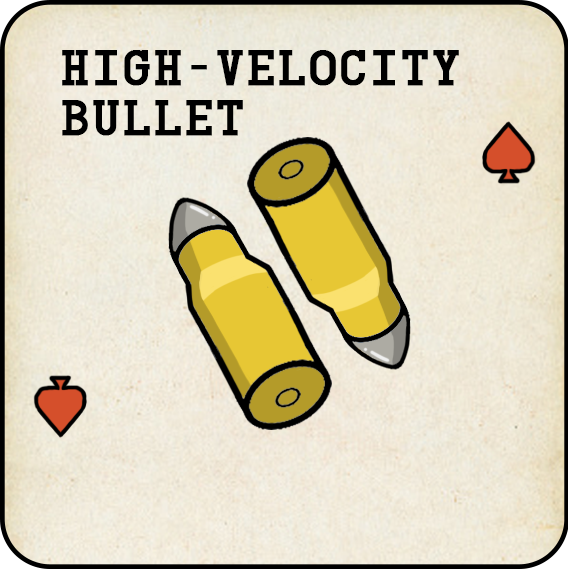
\includegraphics[width=0.3\textwidth]{highVB.png}
    \caption{Beispiel: \quoted{High Velocity Bullet}}
\end{figure}


\quoted{Deputies Bullet} hat den Effekt, dass wenn sie im Revolver platziert wird, die Karte welche sich im Slot 3 befindet wieder in die Hand
zurückgegeben wird. Auch hier kommt das bereits erwähnte Placement Matters ins Spiel, da der Spieler sich bewusst sein
muss, welche Karte auf seine Hand zurückgegeben wird, bevor er \quoted{Deputies Bullet} spielt. Zuerst wird der Spieler den
Effekt von \quoted{Deputies Bullet} als etwas Negatives sehen, um den erhöhten Schaden der Bullet auszugleichen,
eine bewusste Entscheidung, die später noch einmal ins Spiel kommt.

\begin{figure}[H]
    \centering
    
\includegraphics[width=0.3\textwidth]{deputiesB.png}
    \caption{Beispiel: \quoted{Deputies Bullet}}
\end{figure}

Kombiniert mit \quoted{High Velocity Bullet}, kann der eher negative Effekt von \quoted{Deputies Bullet} verwendet werden, um
\quoted{High Velocity Bullet} den Revolver verlassen zu lassen und damit vorzeitig dem Gegner Schaden zuzufügen.
Zusätzlich dazu, dass der Effekt von \quoted{Deputies Bullet}, umgangssprachlich \quoted{Bounce} genannt, \quoted{On-Leave} Effekte triggert,
ist es eine Möglichkeit Karten mit einem \quoted{On-Placedown} Trigger auf die Hand zu geben. Das erlaubt es, den Effekt damit noch einmal zu aktivieren.
Eine andere Möglichkeit ist, dass der Spieler auf eine \quoted{Purge Bullet} stößt. \quoted{Purge Bullet} hat ähnlich wie \quoted{Deputies Bullet}
erhöhten Schaden, dafür ist ihr Effekt, die Zerstörung von zwei Bullets neben ihr, wenn sie platziert wird.
Dies kann jedoch vom Spieler vermieden werden indem er - wieder durch Placement Matters- \quoted{Purge Bullet} auf eine Art und
Weise in den Revolver platziert, sodass keine Karte neben ihr liegt und damit auch nicht zerstört wird.
Ähnlich wie bei \quoted{Deputies Bullet} jedoch, kann \quoted{High Velocity Bullet} mit \quoted{Purge Bullet} zerstört werden, was wiederum als
Verlassen des Revolvers zählt, also den Effekt von \quoted{High Velocities} Bullet aktiviert. \quoted{Purge Bullet} ist außerdem Teil
des Destroy Archetypes, welcher darauf abzielt, dass Karten im Revolver zerstört werden.
Dieser relativ abgesonderte Archetype, kann trotzdem mit \quoted{On-Leave} Effekten kombiniert werden, was wiederum das breite
Kartendesign von \FF veranschaulicht.

\begin{figure}[H]
    \centering
    
\includegraphics[width=0.3\textwidth]{purgeB.png}
    \caption{Beispiel: \quoted{Purge Bullet}}
\end{figure}


Der breite Ansatz ermöglicht es dem Spieler, mit fast jeder neuen Karte, die er erhält, neue Kombinationen und Nutzungsmöglichkeiten zu entdecken.
Es stärkt außerdem das Verständnis der Spielmechaniken.
Jedoch funktionieren nicht alle \FF Archetypen mit jedem anderen, es würde sonst den Spaß aus dem Deckbau nehmen.
Wäre das nämlich der Fall, wäre das Bauen eines Decks komplett obsolet und der Spieler müsste sich keine Gedanken darüber machen, wie er sein Deck zusammenstellt.



\subsection{Kartensammeln und Kartenpools}\label{subsec:placementMatters}

Durch die Vielzahl an Karten und den Unterschieden in der Komplexität zwischen diesen Karten werden Karten in \FF in \quoted{Pools} eingeteilt.
Diese Kartenpools dienen der Kontrolle, wann welche Karten vom Spieler nutzbar sind.
Sie halten komplexe und zu starke Karten vom Spieler fern, bis dieser bereit ist, sie zu erhalten.
Zum jetzigen Zeitpunkt gibt es zwei Kartenpools mit jeweils rund 25 Karten. Combos in Pool eins sind oft einfachere
Versionen der komplizierteren Combos, die durch Pool zwei Karten möglich sind.
Pool eins ist darauf ausgelegt, dass die Grundmechaniken von \FF dem Spieler bewusst werden.
%pool, draft usw


\subsection{Backback und Deck Gamedesign}\label{subsec:placementMatters}

Am Anfang des Spiels besitzt der Spieler sieben bis acht Bullets. Im Laufe des Spiels, sei es durch absolvierte Kämpfe
oder Map-Events, sammelt der Spieler Bullets. Wenn eine Bullet gesammelt wird, kann der Spieler sich entscheiden,
ob er die Karte in sein Deck gibt oder in den Rucksack. Hat er jedoch die Mindestanzahl an Bullets in seinem Deck
noch nicht erreicht, steht ihm nur das Hinzufügen zum Deck offen. Erst wenn der Spieler genug Bullets gesammelt hat,
um die Mindestanzahl des Decks einzuhalten, kann er Bullets aus dem Deck verschieben.


Es gibt einige Faktoren in \FF, die das Bauen bzw. die Wahl des Decks beeinflussen. Zwei kriterien sind die bereits erwähnten Pools und Archetypen.
Je nachdem, wie viele Bullets von einem bestimmten Archetyp ein Spieler besitzt, ist sein Deck mehr ausgeprägt oder weniger.
Die fehlenden Karten des Archetyps können aufgefüllt werden durch andere Karten, die ins Deck passen oder generell immer nutzbar sind.


Das Deckdesign in \FF basiert auf dem sogenannten \quoted{Drei Säulen Modell}.

%mindestanzahl deck
%deckbauen, und wie es beinflusst wird durch pools und encounter modifier

\subsection{Das drei Säulen Modell}\label{subsec:placementMatters}

Das Drei-Säulen-Modell bezieht sich auf die drei \quoted{Arten} von Bullets, die in einem idealen Deck vorhanden sein sollten.
Diese Säulen werden auch beim Designen der Archetypen beachtet, um sicherzustellen, dass jedes Deck über die nötigen
Möglichkeiten verfügt, alle drei Säulen zu erfüllen. Diese Säulen sind ein internes Konzept.
Der Spieler baut Decks nach dem Säulenkonzept automatisch und durch Ausprobieren, da ihm mit der Zeit bewusst wird,
dass ihm \zB die Handkarten immer ausgehen und er dementsprechend Maßnahmen ergreift. Dieses richtige Deckbauen
ist auch Teil der Schwierigkeit von \FF, genauso wie das Meistern der Mechaniken. Jede dieser Säulen hat außerdem sogenannte \quoted{Staples}.
Also Karten, die in jedem Deck gut sind und auch immer in Decks gegeben werden sollten, falls möglich.


Die erste Säule: Ressourcen:
Die Säule der Ressourcen bezieht sich auf Karten, welche dem Spieler einen Vorteil verschaffen. Darin ist der bereits
erwähnte \quoted{Value} inkludiert, also das Ziehen von Karten und die Erzeugung von Reserven. Dadurch verschafft sich der Spieler einen Vorteil,
da mehr Karten in der Hand mehr Möglichkeiten für Züge bedeuten und die extra Reserven auch das Spielen dieser Extrakarten ermöglicht.
Anders gesagt erlaubt die Ressourcen-Säule dem Spieler mehr in weniger Zügen zu spielen.
Staples inkludieren \quoted{Silver Bullet}, in späteren Pools auch \quoted{Gold Bullet} für das Ziehen von Karten und \quoted{Worker Bullet} für das Erzeugen von Reserven.
Je nach Archetyp gibt es auch Karten, welche die Rolle der ersten Säule in ihrem jeweiligen Archetyp übernehmen.
Siehe zum Beispiel \quoted{Gravediggers Bullet} für den Destroy-Archetyp.

\begin{figure}[H]
    \centering
    
\includegraphics[width=0.3\textwidth]{silverB.png}
    \caption{Beispiel: \quoted{Silver Bullet}}
\end{figure}

\begin{figure}[H]
    \centering
    
\includegraphics[width=0.3\textwidth]{goldB.png}
    \caption{Beispiel: \quoted{Gold Bullet}}
\end{figure}

\begin{figure}[H]
    \centering
    \includegraphics[width=0.3\textwidth]{workerB.png}
    \caption{Beispiel: \quoted{Worker Bullet}}
\end{figure}

\begin{figure}[H]
    \centering
    \includegraphics[width=0.3\textwidth]{graveB.png}
    \caption{Beispiel: \quoted{GravediggersBullet Bullet}}
\end{figure}


Die zweite Säule: Schutz:
Die Säule des Schutzes beschäftigt sich damit, gegnerische Angriffe abzuwehren. Dazu gehören Bullets, die dem Spieler
Schutz geben oder besonders stark beim Parieren sind. Schutz ist die kleinste und unwichtigste Säule der drei,
da jede Bullet die Möglichkeit bietet, mit ihr zu parieren und damit Schaden abzuwehren. Jedoch sind auch einfach nur große,
starke Bullets wichtig, um hohe Angriffe von Gegnern abzublocken. Da jede Bullet parieren kann, gibt es nicht wirklich Staples,
\quoted{Turtle Bullet} ist jedoch die beste Wahl für eine einfache und starke Schutz-Bullet.

\begin{figure}[H]
    \centering
    \includegraphics[width=0.3\textwidth]{turtleB.png}
    \caption{Beispiel: \quoted{Turtle Bullet}}
\end{figure}

Die dritte Säule: Wincon:
Die dritte Säule ist der Kern eines Decks und beinhaltet alle Karten, die dafür verwendet werden, durch die Deckstrategie einen Kampf zu gewinnen.
Das Wort \quoted{Wincon} bezieht sich dabei auf die Wincondition, welche je nach Archetyp des Decks unterschiedlich ist.
Ein Rotation Deck hat andere Karten in der dritten Säule als ein Destroy Deck.
Staples existieren nur in den jeweiligen Archetypen
und nicht in der Gesamtheit der Wincon, auch wenn es einzelne Karten gibt, die so stark sind, dass sie in mehreren Decks verwendet werden können.
Ein Beispiel dafür ist \quoted{Bull et} oder \quoted{Bewitched Bullet}.

\begin{figure}[H]
    \centering
    \includegraphics[width=0.3\textwidth]{bewitched_Bullet.png}
    \caption{Beispiel: \quoted{Bewitched Bullet}}
\end{figure}

\begin{figure}[H]
    \centering
    \includegraphics[width=0.3\textwidth]{bull_et.png}
    \caption{Beispiel: \quoted{Bull et}}
\end{figure}

\subsection{Encounter modifier? Was steck dahinter?}\label{subsec:placementMatters}

Der Spieler hat die Möglichkeit, mehrere Decks zu bauen und zwischen bis zu fünf Decks hin und her zu wechseln.
Um den Spieler dazu zu bringen, auch mal ein anderes Deck zu spielen und nicht immer das selbe, und um mehr
Abwechslung ins Spiel zu bringen, wurden Encounter Modifier eingeführt.
Diese Modifier ändern die Spielregeln mal leicht, mal schwer und je nachdem haben große Auswirkungen darauf, wie der Spieler das Spiel spielt.
Ein Beispiel für einen Modifier, welcher das Ändern des Decks als Ziel hat, ist \quoted{Moist}. Durch \quoted{Moist} verliert jede Bullet einen Dmg ihrer Dmg-Value,
wenn sie im Revolver rotiert.
Das wirkt sich vor allem auf Decks aus, welche auf Rotationen basieren. Diese Decks sind noch immer spielbar, jedoch geschwächt.
Ein Beispiel für einen Encounter Modifier, welcher mehr Abwechslung ins Spiel bringt, ist \quoted{Steel Nerves}.
\quoted{Steel Nerves} führt
einen Timer ein, welcher, falls er Null erreicht, den Revolver automatisch schießt. Das bringt einen gewissen Zeitdruck
ins Spiel und der Spieler muss mit der Stresssituation umgehen und dabei weiterhin versuchen, gute Züge zu spielen, um den Gegner zu besiegen. %TODO Bilder von Encounter Modifier

\subsection{Enemy Gamedesign and difficulty scaling}\label{subsec:placementMatters}

Der Gegner ist ein wichtiger Teil des Gameplays von \FF. Er dient nicht nur als Ziel für die Angriffe des Spielers, ohne ihn gäbe es kein Gameplay.
Der Gegner reagiert nicht auf den Spieler, sondern der Spieler reagiert auf den Gegner. Der Gegner zeigt seine nächste Aktion über seinem Kopf an, noch während der Spieler am Zug ist.
Das bewirkt, dass der Spieler seinen Zug anpasst, je nachdem was der Gegner plant. Jedoch kann der Spieler die Pläne des Gegners auch einfach ignorieren,
falls er gerade andere Spielzüge vorbereitet oder glaubt, dass die Aktion des Gegners ihm keine Probleme bereitet.


Ein Gegner kann verschiedene Aktionen ausführen, dazu zählt Schaden zu verursachen, welcher von dem Spieler pariert
werden kann, sich selbst Schild zu geben oder eine gegnerspezifische Aktion auszuführen. Der Gegnertyp bestimmt,
wie viel Schaden der Gegner macht, wie viel Schild er sich selbst geben kann und welche Aktionen er ausführen kann.
Die Witch zum Beispiel kann den Revolver des Spielers nach links drehen.


Gegnertypen sind in verschiedene Klassen eingeteilt,
was durch ihre Effektivität in verschiedenen Kampfszenarien bestimmt wird. Der Pyro ist ein Support-Gegner, da er vor
allem zusammen mit anderen Gegnern glänzt, da er den Spieler in Brand setzt, damit die anderen Gegner mit ihren Angriffen
mehr Schaden machen. Außerdem sorgt die Aktion \quoted{Hot Potato} dafür, dass dem Spieler die Reserven knapp werden. \quoted{Hot Potato}
gibt dem Spieler \quoted{Scorching Bullet} in die Hand, eine feindliche Bullet, welche dem Spieler zehn Schaden verursacht immer am
Ende eines Zuges, falls sich \quoted{Scorching Bullet} in der Hand des Spielers oder im Revolver befindet. Sie kostet drei Reserves,
bekommt der Spieler sie also in die Hand, muss er sich entscheiden, ob er die Bullet behält und seine Reserves für etwas anderes
verwendet oder er die drei Reserves bezahlt und die Bullet damit in den Revolver lädt und wegschießt.


Die Gegner sind so konfiguriert, dass oft Schaden durchgeht, selbst wenn der Spieler etwas pariert. Die Mindestanzahl
an Schaden ist sieben, da die normale Bullet sechs Schaden macht, also die Anfangskarten nicht ausreichen, um den gesamten
Schaden zu parieren. Gegner sind außerdem in Phasen eingeteilt, wobei jede Phase immer mehr Schaden macht als die letzte.
Das wird gemacht, damit der Spieler am Anfang des Kampfes sich ein Spielfeld aufbauen kann, und er weniger Schaden bekommt,
wenn er ein gutes Deck hat und damit den Gegner in wenigen Zügen schon besiegen kann oder sich eine Combo aufbauen kann,
um den erhöhten Schaden irgendwie zu verhindern. Das spielt wiederum mit dem Genre des Rogue-Lites zusammen,
da der Spieler am Anfang des Spiels schlechter sein soll als wenn er schon länger spielt oder schon ein oder zwei Mal gestorben ist.


Gegnertypen sind oft um eine Mechanik konzipiert und dienen oft als Gegenstück zu bestimmten Archetypen oder unterstützen
sogar manchmal Archetypen, wie \zB die Witch, die durch das Linksdrehen des Revolvers dem Rotations-Archetyp hilft.


Kämpfe sind in einer Encounter-Konfigurationsdatei definiert, die basierend auf dem Fortschritt des Spielers passende
Kämpfe aus der Liste auswählt. In dieser Datei werden auch Encounter-Modifiers definiert, damit die Schwierigkeit
der Kämpfe besser kontrolliert werden kann. Außerdem können damit illegale Encounter-Modifier-Kombinationen verhindert
werden, also Kombinationen, die nicht miteinander funktionieren. Je näher der Spieler an der nächsten Area ist,
desto schwieriger werden die Kämpfe. Kämpfe sind so definiert, dass falls ein neuer Gegnertyp das erste Mal vorkommt,
zumindest einmal ein Kampf von dem Spieler absolviert wird, bei dem er nur gegen diesen neuen Gegnertyp kämpft.


Auch wenn an den Gegnern und deren \quoted{Difficulty Balancing} seit schon einem jahr gearbeitet wird, gibt es noch immer viele
zu tun und zu verbessern, da das spiel im Moment zu einfach ist.



\subsection{Carddescriptions}\label{subsec:placementMatters}

Wichtig in einem Kartenspiel wie \FF sind die Beschreibungen der Effekte der Karten. Die Terminologie der Beschreibungen
soll konsistent, verständlich und so kurz wie möglich sein, ohne dass Informationen dabei verloren geht. Bei \FF sind
Effekt Trigger Wörter, welche mit Bindestrichen zusammengehängt werden. Sie sind verknüpft mit dem Wort \quoted{on} am Phrasen Anfang, um zu symbolisieren,
dass der Effekt \quoted{on}, also auf diesem Event getriggert wird. Zusätzlich soll der Trigger auch verständlich sein ohne ihn zu erklären.
\quoted{On-Placedown} zum Beispiel aktiviert den Effekt, wenn die Bullet in den Revolver gelegt wird, also \quoted{down geplaced} wird.
Diese Art von Trigger wird intern \quoted{Major Trigger} genannt.


Übergeordnet über den \quoted{Major Triggern} sind die \quoted{Trigger Conditions}.
Sie werden zuerst gecheckt, wie zum Beispiel die \quoted{While in Revolver:} Condition.
Der nachfolgende \quoted{On-Turn-Begin} Trigger kann nur getriggert werden, wenn die Condition erfüllt ist, also wenn die Bullet sich im Revolver befindet. %TODO Bild von workers Bullet Effekt hier


Sogenannte \quoted{spezifische Trigger} werden ausgeschrieben, da sie zu lang, zu spezifisch und zu selten für die Schreibweise der \quoted{Major Trigger} sind. Ein Beispiel dafür ist
\quoted{Whenever this rotates into the slot that it was originally placed into:}.


Zusätzlich zu abgekürzten Trigger-Bezeichnungen gibt es Keywords. Keywords in \FF sind Effekte, die immer die gleiche
Erklärung haben und deswegen wird die Erklärung in eine extra Info-Box ausgelagert.
Keywords sind ein guter Weg, erfahrenen Spielern die Infos auf einem Blick zu geben, da sie bereits grob wissen, was das
Keyword bedeutet, trotzdem aber neuen Spielern die Möglichkeit zu bieten, sich die Erklärung noch einmal durchzulesen.
Keywords werden angewendet bei \quoted{Trait-Effekten} und \quoted{Status-Effekten}. Trait-Effekte sind extra Eigenschaften für Bullets
wie zum Beispiel \quoted{spray}, durch welchen alle Gegner von der Bullet getroffen werden anstatt nur einer.
Um Status-Effekte und Trait-Effekte variabel zu halten, werden Parameter verwendet. %TODO Bild mit Erklärung zu Parametern noch



%keywords -> für flvor und damit der psiler der schon läänger spielt nicht immer alles lesen muss. und statuseffekte---------------------------------------------------------------------------------------------
%Slots und sloticons


%\subsection{Tutoriel}\label{subsec:placementMatters}


%Broad Bullet design für draft

%

%gegner gamedesign :((((

\subsection{Wie eine Entscheidung das Spiel verändert am Beispiel des Kartennachziehens}\label{subsec:placementMatters}

Während der Entwicklung eines Kartenspieles müssen viele Entscheidungen getroffen werden, wie \zB die Entscheidung,
Karten, welche geschossen wurden nun wieder unter das Deck zu legen. In früheren \FF Versionen wurden geschossene Karten einfach aus dem Kampf entfernt.
Jedoch waren die Kämpfe dadurch relativ schnell vorbei für den Spieler, da nur mehr normale Bullets gezogen wurden nachdem das Deck leer gezogen wurde.
Dadurch das das Deck nach der Änderung nie leer wird, bleibt der Kampf interessant.
Das Spiel wurde auf einen Schlag viel dynamischer und es konnten viel mehr verschiedene und stärkere Combos ausgeführt werden. Das \quoted{Cyclen}
von Karten ist wichtig, da Karten dadurch in einem Kampf öfters verwendet werden können. Decks sind abwechslungsreicher und das Potenzial der Bullets
kann besser von dem Spieler benutzt werden.


Diese simple Änderung zeigt, dass auch nur die kleinste Entscheidung das Spiel komplett verändern kann, weshalb Playtesting
wichtig für ein Spiel wie \FF ist. Dies wurde auch bei der technischen Umsetzung bedacht, weshalb \FF über so viele Configfiles verfügt.


\subsection{Gameplay-Reworks}\label{subsec:placementMatters}
Über die Entwicklung von \FF gab es viele verschiedene Versionen, manche mit kleinen Änderungen, manche jedoch mit komplett veränderten Mechaniken und Regeln.
Die Entwicklung der jetzigen Version zog sich über 2 Jahre.


Unter anderem wurde das damalige Schutzsystem der Cover-Karten mit dem jetzigen Parry-System ausgetauscht.
Cover-Karten waren ein zusätzlicher Kartentyp zu den Bullets, hinter welchen sich der Spieler \quoted{verstecken} konnte.
Bei Tests gab es jedoch einige Probleme mit den Covern, da sich die Spieler immer nur hinter den Covern versteckten
und dadurch eine passive Spielweise unterstützt wurde. Um diesem Problem entgegenzuwirken, wurde die Parry-Mechanik eingeführt,
welche auch Bullets zum Schutz des Spielers verwendet, um sich mehr auf den Kern von \FF - die Bullets - zu konzentrieren.
Das Einführen von Parry markiert den Start der jetzigen \FF Version.

% resets author
\renewcommand{\kapitelautor}{}


\section{Methoden}\label{sec:methoden}

\renewcommand{\kapitelautor}{Autor: Philip Jankovic}

%

\subsection{Kreativfindungsmethoden}\label{subsec:kreativfindungsmethoden}

Während der entwicklung von \FF werden verschiedenste eigene Kreativfindungmethoden verwedet. Diese werden nicht wirklich
geplannt oder eingeleitet, sondern kommen eher an verschiedenen Zeitpunkten. Was sie jedoch verbinden, ist eine zusätzliche
tätigkeit, welche verrtraut ist und die schon so gut gekonnt wird, das sie auch "automatisch" gemacht werden kann.
Dazu gehören \zB Autofahrten, duschen oder Skifahren. Außerdem wird sich viel an der welt rund herum inspieriert.
Konzepte, welche in der echten welt zu finden sind, sind der grundstein von \FF's kreativfindung.

"Good ideas come from one's life experience, losing interest in the world means losing the ability to come up with ideas.
If you're always able to maintain interest in something, and keep your antennea poised to pick up on and react with openess
to the occurences around you, you won't run out of ideas."%TODO QUELLE


Dieses Zitat ist eine große inspiration für Philip Jankovic. Es beschreibt gut, weshalb er gern reist und sich die welt
anschaut und er dadurch auf seine Ideen kommt. Fast alle Bullets in \FF hatten zuerst einen Namen und der Effekt wurde
im nachhinein hinzugefügt, falls ein passender gefunden wurde.


\subsection{Zahlen verändern und Usability Tests}\label{subsec:usability}

Bei der enticklung eines Kartenspieles müssen imens viele änderungen über den Lauf der entwicklung gemacht werden.
Bei \FF wurde eine Kreislauf von Definieren und Testen festgelegt. Oft wird die ursprüngliche Zahl, sei es kosten,
schaden oder gegnerangriffe grob festgelegt. Wenn der neue Build fertig ist, wird geschaut ob die Zahlen passen, aufgeschrieben und danach
je nachdem angepasst. Es werden sich jedoch bei der urspünglichen definition neuer Effekte und Zahlen gedanken gemacht.
\zB Werden Bullets, welche indirekten Schaden durch \zB On-Turn-Beginn machen, wie "Unpleasent Gradient Bullet", einen niedrigen Schaden als andere Bullets.
je nachdem welchen Effekt die Karte haben werden kosten und dmg angepasst.

% kreativfindung und brainstorm methoden


% araki zitat über kreativität

% Inspirationen
%

% resets author
\renewcommand{\kapitelautor}{}


\section{Artstyle}\label{sec:artstyle}

\renewcommand{\kapitelautor}{Autor: Philip Jankovic}

\FF in game visuals sind handgezeichnet und oft statisch. Beim Zeichnen wurde zuerst eine "Reference" gesucht.


\subsection{References}\label{subsec:references}
References beim Zeichnen sind Bilder oder andere Artworks an denen sich orientiert wird. Vorallem am Anfang ist das
Arbeiten mit References fast ein Muss, da das einfache Vorstellen der Zeichnung im Kopf und das anschließende Zeichnen davon höchst anspruchsvoll ist.
Die Perspektive, Kleidung und Körperposen können von der Reference inspieriert werden.
Jedoch wird versucht die Reference nicht 100\% abzuzeichnen, sondern auch den eigenen Stil hinzufügen. \zit{referance}


Für \FF wurden References von "Pinterest", jedoch auch Inspirationen aus diversen Filmen und anderen Medien gesucht. \zit{pinterest}


Ein Beispiel für die Nutzung verschiedenster References ist der Manga \quoted{JOJO's Bizzzar Adventure} von Hirohiko Araki\zit{jojo},
welcher auch eine Inspiration für einige Teile von \FF ist. Nicht nur im Bezug auf die Zeichnungen, sondern auch auf die von dem Autor benützen Krativfindungsmethoden.
Mehr dazu kann in dem Kapitel \ref{methoden} gelesen werden.
Araki verwendet eine große Auswahl als References für seine Zeichnungen, vorallem aus der Welt
der Fashion, was auch in seinem Artstyle zu sehen ist.


\FF bezieht euch ein paar References von "JOJO's Bizzzar Adventure", jedoch ist die Auswahl der benützen References groß und abweichslungsreich.
Auch eigene selbst aufgenomme Reference-Bilder wurden verwenedet für \zB den Main-Charackter des Spieles.





Bei dem Nutzen einer Reference muss jedoch darauf geachtet werden, das Bild nicht nur abzuzeichnen. Je nach Zeichenstil
oder wie stilisiert ein Zeichenstil ist, besteht eine Gefahr, ein Bild nur abzuzeichnen, anstatt es als Reference zu verwenden.
Das Bewahrens eines eigenen Zeichenstiles ist dabei besonders wichtig.


\subsection{Artsytle von \FF}\label{subsec:artsytle}

Der Artstyle von \FF ist im Comic-stil gehalten, mit groben, Bleistift Outlines und Coloring auf der Ebene darunter.
Coloring wird mit einem Farbpinsel auf 100\% Fluss gemacht, damit die Kanten schön hart sind und es sich besser von dem Hintergrund abheben.
Auch wenn die Zeichnungen selber nicht realistisch gezeichnet sind, halten sie sich an realistische Posen und Propertionen, sind also nicht wirklich stilisiert.
Das Spiel nimmt sich dadurch nicht zu ernst, passt aber gut zu dem rauen Wild-West Setting und schlägt für den Betrachter trotz all dieser komischen Bullets
einen Anker in der Realität.

\begin{figure}[H]
    \includegraphics[width=50\%]{artstylepic.jpg}
    \caption{Beispiel: Artstyle von \FF}
\end{figure}


Um den Zeichnungen mehr Tiefe zu geben wird über der Color-Ebene eine Muliplate-Ebene auf 50\% Oppacity verwendet um Schatten
darzustellen. Geshaded wird mit dem selben Pinsel mit welchem Gecolored wird. Das Shading bleibt bei diesem einen grauen ton,
härtere shadows werden durch "Crosshatching" mit dem Outline-Bleistift gemacht.\zit{crosshatching}

\begin{figure}[H]
    \includegraphics[width=50\%]{crossha.jpg}
    \caption{Beispiel: Crosshatching in \FF}
\end{figure}

%
% evolution der artstyles


%artstyle
%

% resets author
\renewcommand{\kapitelautor}{}


%
\chapter{Programmaufbau}\label{ch:programmaufbau}

\renewcommand{\kapitelautor}{Autor: Felix Zwickelstorfer}
\section{Screens}\label{sec:screens}
\renewcommand{\kapitelautor}{Autor: Felix Zwickelstorfer}
In \FF werden grafische Elemente in onj als Teil eines screens definiert.
Dabei sind sich stark voneinander unterscheidende Elemente ein eigener screen, wie \zB der Kampf, die Karte oder der Shop.
Ein screen besteht dabei aus einem root-Element mit untergeordneten child-Elementen.
Zusätzlich hat kann ein screen einen screen-controller haben, welcher für die Verwaltung des screens zuständig ist und komplexere Aufgaben in diesem durchführt.

Im Folgenden werden die einzelnen Bestandteile genauer erklärt und als Beispiel ein Teil des  \inlineCode{HealOrMaxHPScreen} genommen.
Bei diesem kann sich der Spieler entweder heilen oder seine maximale Lebensanzahl erhöhen.
\begin{figure}[H]
    \centering
    \includegraphics[width=0.8\textwidth]{healormaxhpevent.png}
    \caption{Screenshot des HealOrMaxHP-Screens}
\end{figure}
% TODO test if now the intendations are working with this image

%! Author = felix
%! Date = 17/03/2024

\renewcommand{\kapitelautor}{Autor: Felix Zwickelstorfer}
\subsection{Widgets}\label{sec:widgets}
\renewcommand{\kapitelautor}{Autor: Felix Zwickelstorfer}
Ein widget beschreibt jedes Element, welches auf einem screen sichtbar ist. 
Die meisten werden von jedem screen gebraucht, wie \zB das box-widget, welches eine flexbox darstellt, oder auch ein Bild oder ein Text. 
Diese werden im Folgenden als gewöhnliche widgets bezeichnet. 
Es gibt allerdings Elemente, die durch ihre Komplexität oder Dynamik nicht als eine Schachtelung von anderen Elementen dargestellt werden können. 
Diese werden zu ihrem eigenen widget, welches vom controller verwaltet wird, wie \zB die Map.
\renewcommand{\kapitelautor}{Autor: Felix Zwickelstorfer}
\subsubsection{Widgets in Onj}\label{subsubsec:widgetsinonj}
\renewcommand{\kapitelautor}{Autor: Felix Zwickelstorfer}

Alle widgets sind definiert in \inlineCode{assets/onjschemas/screen.onjschema}.
Als Beispiel folgt nun das grüne Icon in der Mitte:
\begin{codeBlock}{onj}{Beispiel: Definition eines Images aus heal\_or\_max\_screen.onj}
    $Image {
        name: "heal_icon",
        textureName: "map_node_heal",
        zIndex: 160,
        scaleX: 1.0,
        scaleY: 1.0,
        styles: [
            {
                positionType: positionType.absolute,
                positionTop: 19#percent,
                positionLeft: 47.15#percent,
            }
        ],
    }
\end{codeBlock}
Es gibt diverse Parameter, die nur für images existieren, während andere "widget shared keys" sind, \dah, dass sie für alle gewöhnlichen widgets verfügbar sind.
Diese beinhalten in dem oben angeführten Beispiel "name", "zIndex" und "styles".
Styles werden bei \ref{subsec:stylesystem} genauer beschrieben.
Es gibt allerdings auch die keys "behaviours" und "dragAndDrop", welche das Verhalten beim Interagieren des Benutzers definieren.

Ein Beispiel für ein spezielles widget ist der Backpack:
\begin{codeBlock}{onj}{Beispiel: Backpack-Widget aus screens.onjschema}
    $Backpack {
        cardsFile: string,
        backpackFile: string,
        deckNameWidgetName: string,
        deckSelectionParentWidgetName: string,
        deckCardsWidgetName: string,
        backPackCardsWidgetName: string,
        backpackEditIndicationWidgetName: string,
        sortWidgetName: string,
        sortReverseWidgetName: string,
        ...widgetSharedKeys,
         children?: $Widget[],
         partOfSelectionHierarchy?: boolean,
    }
\end{codeBlock}
Der Rucksack ist eigentlich nur eine box mit erweiterten Funktionen.
Man kann Kartendecks bauen, benennen und die Karten außerhalb des Decks, der sogenannten Kartenablage, nach gewissen Kriterien sortieren.
Dadurch, dass es ein eigenes widget ist, kann und wird es auf mehreren screens verwendet.
Es beinhaltet alle keys, die auf eine box hat (alles ab den "widget shared keys"), und zusätzlich die Namen zu bestimmten Konfigurationsdateien (cards und backpack), um die Daten richtig darzustellen.
Diese werden mitgegeben, da es eine schönere Lösung ist, als die Pfade hartkodiert im Code stehen zu haben.
Weiteres hat es noch und zusätzlich die Namen bestimmter child-Elemente.
Diese Elemente werden statt von dem screen-controller, von dem Backpack widget verwaltet oder verwendet.

\renewcommand{\kapitelautor}{Autor: Felix Zwickelstorfer}
\subsubsection{Widgets in Kotlin}\label{subsubsec:widgetsinkotlin}
\renewcommand{\kapitelautor}{Autor: Felix Zwickelstorfer}
Bei LibGdx ist ein widget immer ein \inlineCode{com.badlogic.gdx.scenes.scene2d.Actor} oder eine Unterklasse davon.
In Forty-Five werden keine der Klassen von LibGdx direkt verwendet, sondern immer eigene Erweiterungen, wegen des style-Systems wie bereits oben beschrieben.
Weiteres werden sie benötigt, um eigene events verarbeiten zu können, wie das hover-event.
Programmtechnisch gibt es vier Hauptänderungen, die überschrieben werden:
\begin{enumerate}
    \item Die ``layout'' Funktion, welche beschreibt, wo welche Elemente positioniert sind und bei Boxen auch deren Kinderelemente.
    \item Die ``draw'' Funktion, welche für die Darstellung verantwortlich ist. Das ermöglicht es, shader hinzuzufügen oder das style-System einzubauen.
    Sie wird jeden Frame einmal ausgeführt und wird daher ebenfalls zum Updates von timelines (siehe~\ref{subsec:timelines}) verwendet.
    \item Interfaces werden hinzugefügt, welche einerseits für das style-System verwendet werden, als auch generell das Arbeiten mit widgets vereinfacht.
\end{enumerate}
\renewcommand{\kapitelautor}{Autor: Felix Zwickelstorfer}
\subsubsection{Templates}\label{sec:templates}
\renewcommand{\kapitelautor}{Autor: Felix Zwickelstorfer}
Templates sind ein weiterer wichtiger Part von widgets, da sie das dynamische Erstellen von Elementen im Code erleichtern.
Außerdem verbessern sie die Lesbarkeit des Codes, da sehr ähnliche widgets als ein template mit mehreren Parametern definiert werden können.
Alle gewöhnlichen widgets können als template erstellt werden.
Dies wird vor allem bei Karten verwendet, da das Design und das Verhalten innerhalb eines screens für die Karten meistens gleich ist.
Deshalb erstellt man ein widget aus einem template und es wird nur das Bild und der hover-text auf die entsprechende Karte angepasst.
Templates werden allerdings auch an vielen anderen Stellen verwendet, \zB bei den Warnungen und Hinweisen im Backpack, als auch bei dem HealOrMaxHP-screen für die beiden auswählbaren widgets.
Ein template zeichnet sich dadurch aus, dass es zusätzlich zu den normalen keys noch einen "template name" und die "template keys" hat.
Diese sehen bei dem Beispiel screen folgendermaßen aus:
\begin{codeBlock}{onj}{Beispiel: Ausschnitt eines Templates aus heal\_or\_max\_screen.onj}
templates: [
    $Box {
        template_name: "healOptionTemplate",
        template_keys: {
            "name": "name",
            "children.1.template": "templateMainText",
            "children.0.textureName": "textureName",
        },
        name: "Die name-value wird überschrieben, weil der zugehörige key in den templates angegeben ist",
        children: [
            $Image {
                textureName: "heal_or_max_add_max_health",
                scaleX: 0.8,
                scaleY: 0.8,
            },
            $TemplateLabel {
                template: "+5 Max HP",
                font: "red_wing_cm",
                color: color.dark_brown,
                fontScale: 1.1,
                align: "center",
            },
        ],
    }
]
\end{codeBlock}
Im Programmcode gibt man, wenn man ein template verwenden will, den template name an, und man gibt ein \inlineCode{OnjObject} mit, das die zu überschreibenden Daten beinhaltet.
In diesem Beispiel sind es der angezeigte Text und das Bild, da diese sich von der linken und rechten Seite unterscheiden.
Zusätzlich wird über das template auch der interne Name des widgets gesetzt.
%! Author = felix
%! Date = 17/03/2024
\renewcommand{\kapitelautor}{Autor: Felix Zwickelstorfer}
\subsection{Parameter}\label{subsec:parameter}
\renewcommand{\kapitelautor}{Autor: Felix Zwickelstorfer}

Jeder screen hat in Onj drei Bereiche.
Diese beinhalten die wichtigsten Informationen für diesen screen und umfassen die logische Verwaltung und Gliederung, aber auch die benötigten Ressourcen.

\renewcommand{\kapitelautor}{Autor: Felix Zwickelstorfer}
\subsubsection{Assets}\label{subsubsec:assets}
\renewcommand{\kapitelautor}{Autor: Felix Zwickelstorfer}
Die assets beschreiben, welche Ressourcen dieser screen immer laden soll. 
Bei \FF werden normalerweise Ressourcen wie Bilder, Animationen sowie Schriftarten nur im screen gespeichert. 
Das heißt, dass sie bei jedem screen neu geladen werden. 
Für diese grundlegenden Elemente gibt man dem screen eine Liste an assets mit.
Manche Ressourcen, wie \zB Karten, werden erst vom Programm geladen, da ein durchgehendes Laden aller Karten zu einer unnötigen Auslastung des RAMs führen würde.
Darauf wird allerdings genauer bei~\ref{sec:resourcenmanagement} eingegangen.

\renewcommand{\kapitelautor}{Autor: Felix Zwickelstorfer}
\subsubsection{Viewport}\label{subsubsec:viewport}
\renewcommand{\kapitelautor}{Autor: Felix Zwickelstorfer}
Der viewport beschreibt die logische Anzahl an "points" pro screen in der Breite und Höhe. 
Man kann diese points mit Pixeln vergleichen, ist allerdings von der eigentlichen Auflösung des Spiels getrennt.
Er wird verwendet, damit Elementen bestimmte Größen im Verhältnis zum screen gegeben werden können.
Zusätzlich wird er verwendet, um bei box-Elementen die child-Elemente zu platzieren.
Diese werden immer nur auf ganzzahlige points gesetzt, wodurch es bei zu niedriger logischer Auflösung zu nicht korrekt platzierten Elementen kommen kann.

\renewcommand{\kapitelautor}{Autor: Felix Zwickelstorfer}
\subsubsection{Optionen}\label{subsubsec:optionen}
\renewcommand{\kapitelautor}{Autor: Felix Zwickelstorfer}
Die Optionen sind der vermutlich wichtigste Parameter eines screens. 
Sie beinhalten einerseits Elemente wie den Hintergrund, sowie Parameter für die Musik.
Andererseits werden auch die input maps mitgegeben, die für einfache User-Interaktionen zuständig sind.
Diese sind genauer in~\ref{sec:key-input-system} beschrieben. 
Das wichtigste Element ist der screen-controller.
Dieser ist das zentrale Steuerelement eines screens und wird bei~\ref{subsec:screen-controller} beschrieben. 
Wie das folgende Beispiel zeigt, gibt man dem screen-controller die Namen bestimmter Elemente mit, welche dieser verwaltet. 
Das erlaubt es die Element-Struktur des screens zu ändern, aber trotzdem noch auf die richtigen Elemente im Code zu referenzieren.

\begin{codeBlock}{onj}{Beispiel: Optionen des HealOrMapHP\-Screens}
options: {
    background: "hover_detail_background",
    transitionAwayTime: 1.5,
    music: "map_theme",
    playAmbientSounds: true,
    inputMap: [
        ...(inputMaps.defaultInputMap),
        ...(inputMaps.healOrMaxInputMap),
        ...(inputMaps.addMaxHPInputMap),
    ],
    screenController: $HealOrMaxHPScreenController {
        addLifeActorName: "add_lives_option",
    }
}
\end{codeBlock}
%! Author = felix
%! Date = 17/03/2024
\renewcommand{\kapitelautor}{Autor: Felix Zwickelstorfer}
\subsection{Screen-Controller}\label{subsec:screen-controller}
\renewcommand{\kapitelautor}{Autor: Felix Zwickelstorfer}
Der Screen-Controller ist die zentrale Steuerungseinheit eines Screens und verwaltet diesen.
Er ist für die gesamte Logik zuständig als auch für die meisten User-Interkationen.
Die einzigen Ausnahmen sind komplexe Widgets (siehe~\ref{sec:widgets}) und InputMaps (siehe\ref{sec:key-input-system}).

Als Beispiel folgen nun Ausschnitte des \inlineCode{HealOrMapHPScreenControllers} erklärt:

\begin{codeBlock}{kotlin}{Beispiel: Screen\-Controller des HealOrMapHP\-Screens}
    override fun init(onjScreen: OnjScreen, context: Any?) {
        val rnd = Random(context.seed)
        if (context !is HealOrMaxHPMapEvent) throw RuntimeException("context for ${this.javaClass.simpleName} must be a ChooseCardMapEvent")
        amount = context.healthRange.random(rnd) to context.maxHPRange.random(rnd)
        TemplateString.updateGlobalParam(
            "map.cur_event.heal.lives_new",
            min(SaveState.playerLives + amount.first, SaveState.maxPlayerLives)
        )
        // ...
    }
\end{codeBlock}

Die \inlineCode{init} Methode wird aufgerufen, nachdem alle Elemente dem Screen hinzugefügt worden sind.
Der context ist ein MapEvent, da dieser Screen nur als Event aufgerufen werden kann.
Das Event beinhaltet Daten wie den Seed des Events oder der Bereiche, die man geheilt wird.
Anschließend berechnet der Screen-Controller die Anzahl, die an Leben hinzugefügt werden kann.
Der Seed ist notwendig, damit diese Zahl immer gleich ist.
Wäre es immer zufällig, könnte man als Spieler in das Event und wieder zum Startbildschirm gehen.
Das könnte man so oft wiederholen, bis man die maximale Anzahl an Leben bekommt.
Der Seed verhindert dies.
Zuletzt aktualisiert der Screen-Controller noch die Zahlen Texte, damit der Spieler auch sieht, wie viele Leben er dazubekommt.

Weiteres kann dieser Screen "completed", also abgeschlossen, werden.
Dafür hat er folgende Methode:
\begin{codeBlock}{kotlin}{Beispiel: Screen\-Controller des HealOrMapHP\-Screens}
    override fun completed() {
        SoundPlayer.situation("heal", screen)
        if ((screen.namedActorOrError(healChosenTarekGeorgWidgetName) as CustomFlexBox).inActorState("selected")) {
            val newLives = min(SaveState.playerLives + amount.first, SaveState.maxPlayerLives)
            FortyFiveLogger.debug(logTag, "Lives healed from ${SaveState.playerLives} to $newLives!")
            SaveState.playerLives = newLives
        }
        // ...
        context?.completed()
    }
\end{codeBlock}

Wenn dieser Screen abgeschlossen wird, sieht man, dass ein Sound abgespielt wird.
Anschließend wird die Option des Spieler überprüft, und falls er sich heilen wollte, werden seine dementsprechend angepasst.
Zum Schluss wird der "context" ebenfalls abgeschlossen, was in dem Fall heißt, dass man zurück zur Map gelangt und dass man dieses Event nicht mehr ausführen kann.
%! Author = felix
%! Date = 17/03/2024

% Preamble
\documentclass[11pt]{article}

% Packages
\usepackage{amsmath}

% Document
\begin{document}



\end{document}

\section{Advanced Text}\label{sec:advanced-text}

\renewcommand{\kapitelautor}{Autor: Irgendwer} % todo: replace

%
% text goes here
%

% resets author
\renewcommand{\kapitelautor}{}


\section{Kampfablauf}\label{sec:kampfablauf}

\renewcommand{\kapitelautor}{Autor: Irgendwer} % todo: replace

%
% text goes here
%

% resets author
\renewcommand{\kapitelautor}{}


\section{Ressourcen- und Speicher-Management}\label{sec:resourcenmanagement}

\renewcommand{\kapitelautor}{Autor: Marvin Kurka}

Kotlin, wie auch Java und andere JVM-basierende Sprachen verwendet einen Garbage Collector, kurz GC, um den
Speicherplatz von nicht mehr verwendetet Objekten freizugeben.\cite{oracleGC}

\subsection{Wie funktioniert Garbage Collection?}

Garbage Collection ist in zwei Phasen aufgeteilt.
In der ersten Phase, dem Marking, werden alle Objekte, für die noch eine Referenz existiert, markiert.
Dabei geht der GC von sogenannten Roots aus, was Objekte sind, auf die das Programm eine unmittelbare
Referenz hat.
Diese werden markiert und der Prozess wird rekursiv für alle Referenzen, die diese Objekte halten, wiederholt.
Am Ende sind alle Objekte, für die das Programm noch eine gültige Referenz hält markiert.
In der zweiten Phase werden alle Objekte, die nicht markiert wurden, und demnach nicht mehr erreichbar sind, gelöscht.
Zusätzlich kann hier eine Defragmentierung stattfinden.\cite{oracleGC}

Eine GC durchzuführen ist teuer.
Erst muss jedes Objekt in der Baumstruktur des Heaps durchgegangen und markiert werden, und dann beim
Löschen/Defragmentieren müssen große Teile des Heaps kopiert werden.
Dazu kommt, dass es sich bei Garbage Collections um "Stop the World Events" handelt.
Da große Teile des GC-Prozesses nicht parallel mit den Application Threads laufen können, muss das
Programm für die Dauer der Garbage Collection pausiert werden, was sowohl die Geschwindigkeit als auch die
Responsiveness des Programms beeinträchtigt.\cite{oracleGC}

Um dieses Problem wenigstens zu mindern, verwendet die JVM eine generational Garbage Collection.
Die meisten Objekte, die in der Laufzeit eines Programms allokiert werden, haben nur eine sehr geringe Lebenszeit,
während einige wenige Objekte signifikant längere Lebenszeiten haben.
Die JVM macht sich das zu Nutze, um den Heap in verschiedene Generation einzuteilen, je nachdem wie viele GCs
ein Objekt schon überlebt hat.
Bei einem Minor Garbage Collection Event werden dann nur die jüngeren Generationen durchsucht, während bei einem
Major Garbage Collection Event der gesamte heap durchsucht wird.\cite{oracleGC}

\subsection{Gargabe Collection in Videospielen}

GC funktioniert am besten mit kleinen Objekten mit kurzer Lebensdauer.
Diese überleben im Idealfall schon die erste minor GC nicht, und müssen deshalb nicht in den Bereich der older
Generation überführt werden.
Außerdem ist das allokieren/kopieren/löschen durch die kleine Größe wenig Aufwand.
Weiters sollten große Objekte im Idealfall nicht im stable State des Programmes allokiert werden, um die Zahl an major
GCs gering zu halten.\cite{infoqJavaPerformance}

Allerdings ist es gerade in Videospielen so, dass es besonders viele sehr große und langlebige Objekte gibt.
Texturen, Animationen und Sounds können oft Megabytes an RAM benötigen und werden oft im stable state des Programms
allokiert, \zB bei einer Screen-Transition.
In Videospielen spielt oft auch die Latenz, also wie schnell auf User-Input reagiert wird, eine wichtige Rolle.
Diese kann durch GC beeinträchtigt werden, da diese die Applikation Thread pausiert und diese dann nicht sofort auf
den Input reagieren könne.

Außerdem werden oft Ressourcen verwendet, die gar nicht von einer konventionellen GC verwaltet werden können, da sie zur
GPU hochgeladen werden müssen.
Das inkludiert \zB Texturen oder Shader.
Solche Ressourcen könnten theoretisch über einen Finalizer, der automatisch läuft, bevor die GC ein Objekt collected,
freigegeben werden, das würde die Performance des GC-Prozesses allerdings weiter verschlechtern.\cite{infoqJavaPerformance}

Ein weiterer Grund, warum man sich bei großen Objekten nicht auf den GC verlassen sollte, ist, dass oft eine feine
Kontrolle über große Ressourcen notwendig ist.
Sollte irgendwo im Programm noch eine einzelne Referenz zu einem Objekt existieren, wird dieses nicht vom GC
eingesammelt, auch wenn es vielleicht nicht mehr verwendet wird.
So können sehr einfach Memory Leaks entstehen, die auch noch sehr schwer zu debuggen sind.
All das macht GC besonders ungeeignet für Videospiele und ist er Grund, warum LibGdx einen anderen Ansatz für das
Managen von großen Ressourcen verfolgt.

\subsection{LibGdx und das Disposable-Interface}

In LibGdx werden große Ressourcen durch nativen Code allokiert und nicht vom GC verwaltet.
Klassen, die solche Ressourcen repräsentieren, implementieren das Disposable-Interface, das die
\inlineKotlin{Disposable::dispose} Funktion zur Verfügung stellt.
Diese muss am Ende des Lebenszyklus des Objektes aufgerufen werden, um den allokierten Speicher wieder freizugeben.\cite{libGdxMemoryManagement}

Diese Herangehensweise macht den effizienten Umgang mit Ressourcen möglich und gibt dem Programmierer Kontrolle über
die Lebenszeit von großen Objekten.
Allerdings führt das auch dazu, dass viele Fehlerquellen, die durch GC eliminiert wurden, wieder auftreten können.
Beispiele sind Memory Leaks, die auftreten, wenn eine Ressource nicht wieder freigegeben wird, oder eine
Use-after-Free-Situation, bei der eine Ressource verwendet wird, obwohl sie eigentlich schon freigegeben wurde, was
zu undefinierten Verhalten führt.\cite{libGdxMemoryManagement}

\subsection{Der ResourceManager}

Gutes Ressourcenmanagement ist in der Spielentwicklung extrem wichtig.
Schlechtes Management kann \zB zu langen Wartezeiten bei Screen-Transitions führen, und so die Immersion brechen.
Aber falscher Umgang mit Ressourcen kann nicht nur das Spielerlebnis verschlechtern, er kann das Spiel sogar
komplett unspielbar machen.
Die im vorherigen Absatz beschriebenen Bugs wie Use-after-Free oder Memory Leaks können zu Crashes oder anderen
Fehlverhalten des Spiels führen.
Deswegen war das Ressourcenmanagement bei der Entwicklung von \FF eine besonders große Herausforderung.
Um diese zu bewältigen wurde der ResourceManager entwickelt, eine Klasse, die Ressourcen über die gesamte
Applikation hinweg verwaltet.

\subsubsection{Grundfunktion des ResourceManager}

Klassen, die Ressourcen vom ResourceManager verwenden wollen, müssen das ResourceBorrower-Interface implementieren.
Dieses enthält keine Funktionen, es dient nur dem Zweck, dem Programmierer zu erinnern, dass diese Klasse Ressourcen
verwendet und diese auch zurückgeben muss.

Eine Klasse, die ResourceBorrower implementiert kann die \inlineKotlin{ResourceManager::borrow} Funktion verwenden,
um sich eine Ressource auszuborgen.
Die Ressource muss zu diesem Zeitpunkt nicht unbedingt geladen sein, sie wird nur als in Verwendung markiert.
Um die Ressource tatsächlich zu bekommen, wird die \inlineKotlin{ResourceManager::get} Funktion verwendet.
Spätestens zu diesem Zeitpunkt wird das Laden erzwungen.
Um die Ressource wieder zurückzugeben, wird die \inlineKotlin{ResourceManager::giveBack} Funktion verwendet.
Auch hier gilt wieder, dass ein Aufruf dieser Funktion nicht unbedingt zum Entladen der Ressource führen muss,
da auch ein zweiter Borrower sie noch verwenden könnte.

Diese zentrale Verwaltung ermöglicht effizientes Management der Ressourcen, da der ResourceManager zu jedem Zeitpunkt
über die Gesamtsituation im Programm Bescheid weiß.
Das ermöglicht es, dass doppelte Laden von Ressourcen oder das Entladen und sofortige neu Laden zu verhindern.

\subsubsection{Das asynchrone Laden von Ressourcen}

Das Laden von Ressourcen ist eine sehr teure Operation, da oft MB-große Dateien zuerst in dem RAM gelesen und
dann zur GPU hochgeladen werden müssen.
Würde das alles synchron mit der Render-Logik auf dem Main-Thread passieren, würde das zu merkbaren Verzögerungen
führen.
Daher war klar, dass das Laden von Ressourcen so weit wie möglich auf einem separaten Thread passieren sollte.
Allerdings war es in der Praxis nicht umsetzbar, alle Ressourcen vollständig von einem anderen Thread aus zu laden.
Grund dafür ist der OpenGL Kontext.
Nur ein Thread kann den OpenGL Kontext halten, und dieser Thread ist im Falle von LibGdx immer der Main-Thread.
Nur dieser kann dann Operation durchführen, die mit OpenGL zu tun haben, wie \zB Grafiken zu rendern, aber auch nur
dieser Thread kann Daten zur GPU hochladen.
Ein Aufruf von \zB dem \inlineKotlin{Texture} Konstruktor von einem Thread ohne OpenGL-Kontext würde zu nicht
definierten Verhalten führen.\cite{libGdxThreading}

Um dieses Problem so gut wie möglich zu umgehen, wurde für jeden möglichen Ressourcen-Typ eine Zwei-Schritt Lade Logik
definiert.
Der erste Schritt kann sicher auf jedem Thread ausgeführt werden, und lädt \zB in Falle einer Textur die Daten als
Pixmap in den RAM\@.
Im zweiten Schritt, der nur auf dem Main-Thread ausgeführt werden darf, passiert der tatsächliche Aufruf des
\inlineKotlin{Texture} Konstruktors und damit der Upload zur GPU\@.
Da auch der zweite Schritt Zeit in Anspruch nimmt, kann es hier zu Verzögerungen beim Rendering kommen, das hat sich
aber leider nicht vermeiden lassen.

\subsubsection{Der ServiceThread}

Der ServiceThread ist ein Thread der zu Beginn des Programms gestartet wird und dann parallel zu diesem läuft.
Er übernimmt mehrere Aufgaben, \zB das Zeichnen der Karten-Texturen, bei weitem die Größte ist aber das Laden von
Ressourcen.
Der ServiceThread kommuniziert mit dem Main-Thread über einen \inlineKotlin{Channel<ServiceThreadMessage>}, über
den der Main-Thread Nachrichten an den ServiceThread schicken kann.
Nach einem Event, bei dem viele Ressourcen ausgeborgt wurden (\zB einer Screen-Transition) wird die
\inlineKotlin{ServiceThreadMessage.PrepareResources} Nachricht and den ServiceThread geschickt.
Dieser startet dann eine Coroutine für jede ausgeborgte, aber nicht geladene Ressource, die diese vorbereitet.
Diese Coroutines werden von Kotlins IO-Dispatcher verwaltet, der diese auf mehrere Worker-Threads verteilt ausführt.

Im Main-Thread wird währenddessen das Laden der Ressource so lange wie möglich herausgezögert, um den ServiceThread
eine möglichst hohe Chance zu geben, die Ressource parallel zu laden.
Ein Image \zB lädt seine dazugehörige Textur erst beim ersten \inlineKotlin{draw()} Aufruf.
Wenn nun ein Zugriff stattfindet, tritt eine dieser Möglichkeiten ein:

\begin{itemize}
    \item Die Ressource war bereits geladen: Der best Case, die Ressource war beim \inlineKotlin{borrow} Aufruf bereits
        in Verwendung und muss nicht geladen werden.
    \item Die Ressource ist vorbereitet: Der ServiceThread hat die notwendigen Daten bereits geladen, nur noch der
        zweite Schritt des Ladevorgangs muss ausgeführt werden.
    \item Die Ressource ist gerade in Vorbereitung: Der Main-Thread muss auf den ServiceThread warten und führt dann
        den zweiten Schritt des Ladevorgangs aus.
        Der Main-Thread blockiert in diesem Zeitraum.
    \item Die Ressource ist nicht geladen: Der worst Case, der komplette Ladevorgang muss auf dem Main-Thread ausgeführt
        werden.
        Der Main-Thread blockiert in diesem Zeitraum.
\end{itemize}

\subsubsection{Das Laden von FrameAnimations}

Aufgrund ihrer besonders hohen Größe haben FrameAnimations ihre eigene Lade-Logik.
So kann verhindert werden, dass Animationen jemals auf dem Main-Thread geladen werden, was zu extremen Lag führen würde.

Zuerst werden die Frames der Animationen in einen Atlas verpackt.
Diese Atlase sind Texturen mit Größen von maximal 4096x4096 Pixeln, die mehrere Frames der Animationen enthalten.
Das minimiert die Anzahl der Texturen, die zur GPU hochgeladen werden müssen.
Das Verpacken der Atlase findet nicht zu Runtime statt, sondern zu Compile-Time, indem ein Gradle-Task ausgeführt wird.

\begin{figure}[H]
    \centering
    \includegraphics[scale=0.5]{example_animation_atlas.png}
    \caption{Beispiel für Animations-Atlas in 20\% der Original-Auflösung}
\end{figure}

Die \inlineKotlin{DeferredFrameAnimation} Klasse implementiert die Lade-Logik für Animationen.
Beim Erstellen einer Instanz dieser Klasse wird eine Nachricht an der ServiceThread geschickt, die diesem befiehlt,
den Atlas mit den Frames er Animation zu laden.
Der ServiceThread startet eine Coroutine auf einem gesonderten Thread nur für Animation, um zu verhindern, dass das
Laden der Animation das Laden anderer Ressourcen, die zeitkritisch sein könnten, blockiert.
Während die eigentliche Animation geladen wird, rendert DeferredFameAnimation ein statisches Preview-Bild,
typischerweise der erste Frame der Animation, um die Ladezeit zu überbrücken.
Nachdem das asynchrone Laden des Atlases abgeschlossen ist, müssen die Texturen dieses Atlases
auf dem Main-Thread zur GPU hochgeladen werden.
Durch die Größe der Texturen führt das zu merkbaren Lag.
Um das zumindest weniger auffällig zu machen, passiert der Upload der Texturen zwischen Render-Zyklen und mit 100ms
Zeitverzögerung zwischen Uploads.

% resets author
\renewcommand{\kapitelautor}{}


\renewcommand{\kapitelautor}{Autor: Felix Zwickelstorfer}
\section{Savestates}\label{sec:savestates}
\renewcommand{\kapitelautor}{Autor: Felix Zwickelstorfer}

In Forty-Five gibt es drei verschiedene Savefiles, die unterschiedliche Daten speichern und diverse Zwecke erfüllen.
Diese sind die permanente und normale Speicherdatei, als auch die User-Präferenzen.
Jedes dieser drei hat eine default Version, welche beim erstmaligen Starten des Spiels geladen und verwendet werden.
Diese werden auch verwendet, falls ein Fehler mit einer aktuell benutzten Datei auftritt.
Die Unterschiede werden im Folgenden näher erklärt.


\subsection{Savefile}\label{subsec:savefile}

Das normale Savefile, das eigentlich nur als Savefile betitelt wird, ist jenes, welches sich über einen einzelnen Run verändert.
Das heißt, während man herumgeht und Karten sammelt, werden diese temporär in diese Datei geschrieben.
Es beinhaltet beispielsweise:
\begin{itemize}
    \item Karten: Welche Karten der Spieler aktuell besitzt.
     Dies beinhaltet auch alle Karten der Decks.
    \item Decks: Die 5 Konfigurierbaren Decks, also den Namen und die Karten mit den jeweiligen Positionen.
    \item Leben: Wie viele Leben der Spieler aktuell hat, als auch die maximale Anzahl der Leben.
    \item Statistiken: Diverse Daten wie \zB die Anzahl der gewonnenen Kämpfe oder der verbrauchten Reserves.
    \item Position: Auf welcher Map und welchem Feld der Spieler steht.
    Zusätzlich dazu auch das davor besuchte Feld, falls man auf einem Kampf steht, welcher einen nur in eine bestimmte Richtung gehen lässt, nämlich zurück.
\end{itemize}


\subsection{permanentes Savefile}\label{subsec:perma-savefile}
Das permanente Savefile wird, wie der Name sagt, eigentlich niemals zurückgesetzt.
Falls diese Datei beim Start des Spiels fehlt, wird es vom Programm wie eine neue Installation gewertet und auch die anderen beiden Speicherdateien werden neu überschrieben.
Es beinhaltet teilweise über scheidende Daten zur normalen Speicherdatei, wie die Karten die man besitzt.
Allerdings werden diese nur dann aktualisiert, falls man in eine neue Area (=Stadt) geht, die man noch nie davor besucht.
Die bereits gesehenen Areas werden auch in dem File gespeichert.
Zusätzlich dazu beinhaltet es noch Daten bezüglich des Tutorials, vor allem welche bereits durchgespielt worden sind.

\subsection{User-Präferenzen}\label{subsec:user-prefs}
Die User-Präferenzen werden ähnlich wie die permanente Speicherdatei eigentlich nur beim erstmaligen Start neu geladen, da man diese meistens nicht ändern will.
Sie beinhalten alles, was man in den Einstellungen ändern kann, also die gewünschte Lautstärke für sowohl die Musik als auch die Soundeffekte als auch auf welchem Screen man nach Starten des Spiels sieht.
Weiteres beinhaltet es die Option, ob der Screen bei bestimmten Aktionen Wackeln darf oder nicht.


\section{Effektsystem}\label{sec:effectsystem}

\renewcommand{\kapitelautor}{Autor: Marvin Kurka}

\FF zeichnet sich vor allem durch die Effekte der Karten aus, die es dem Spieler ermöglichen, komplexe Kombinationen
von Karten zu spielen, um verschiedene Effektketten auszulösen.
Um es möglich zu machen, solche Effekte schnell und einfach zu definieren, wurde ein System entwickelt, dass es
ermöglichen soll, neue Effekte zu definieren ohne viel in vorhandenen Code eingreifen zu müssen.

Effekte werden in zwei Kategorien eingeteilt: Trait Effekte und normale Effekte.
Trait Effekte werden nicht von dem Effektsystem verwaltet und werden für alle Situationen verwendet, in denen das
normale Effetsystem nicht ausreicht.
So gibt es zm Beispiel den "reinforced" Trait-Effekt, der dafür sorgt, dass eine Bullet immer den ganzen Damage
des Gegners parried, unabhängig von ihrem eigenen Damage-Wert.
Da diese Logik von dem Parry-System übernommen werden muss, ist dieser Effekt ein Trait-Effekt und wird somit nicht
über das normale Effektsystem definiert.

Normale Effekte bestehen aus zwei Teilen: dem Trigger und dem Effekt selber.
Der Trigger gibt an, wann der Effekt aktiv wird.
Beispiele sind: \inlineKotlin{ON_SHOT}, \inlineKotlin{ON_ENTER} oder \inlineKotlin{ON_REVOLVER_ROTATION}.
Jedes Mal, wenn der GameController eine Aktion ausführt, die Effekte auslösen könnte, werden alle relevanten Karten
im Spiel auf den zu der Aktion passenden Trigger überprüft.
Trigger können auch kaskadieren, das heißt, wenn \zB die \inlineKotlin{ON_BOUNCE} oder \inlineKotlin{ON_DESTROY}
Trigger ausgelöst werden, wird automatisch auch der \inlineKotlin{ON_LEAVE} Trigger ausgelöst.
Definiert eine Karte einen oder mehrere Effekte für diesen Trigger, wird dieser aktiv.

Die Effekte machen starken Gebrauch von Timelines, die in Kapitel~\ref{subsec:timelines} erklärt sind.
Wird ein Effekt ausgelöst, wird die \inlineKotlin{Effect::onTrigger} Funktion aufgerufen, die eine Timeline zurückgibt.
Diese wird in zusammen mit anderen Timelines, die \zB von anderen Effekten stammen, in eine Timeline eingearbeitet,
die dann ausgeführt wird.
Um das Spiel zu beeinflussen, kann der Effekt einige Funktionen aus dem GameController verwenden, um Timelines
zu bekommen, die \zB den Revolver drehen, oder eine Karte zerstören.

Effekte, die sich auf andere Bullets im Revolver beziehen, verwenden die \inlineKotlin{BulletSelector} Klasse um
auszuwählen, auf welche Bullets der Effekt angewandt wird.
Je nach Definition des Effekts wird dann ein Popup geöffnet, das den Spieler nach einer Target-Bullet für den Effekt
fragt, oder ein anderes Kriterium wird verwendet, um festzustellen, welche Bullets betroffen sind.

Effekte, die Damage-Werte von anderen Karten im Revolver verändern, verwenden die \inlineKotlin{Card.CardModifier}
Klasse.
Diese erlaubt es eine temporäre Damage-Änderung zu definieren, entweder in der Form einer Addition oder der eines
multiplikativen Faktors.
Über den Konstruktor dieser Klasse können auch Lambdas mitgegeben werden, die bestimmen, wann der Modifier wieder
entfernt wird, oder in welchem Zeitraum er gültig ist.
Die Leaders Bullet zum Beispiel gibt allen anderen Karten im Revolver einen Modifier, der abläuft, wenn Leaders Bullet
den Revolver verlässt.
Die +P+ Bullet verwendet dieses System, um sich selbst einen Modifier zu geben, der nur aktiv ist, wenn der Gegner einen
Status Effekt hat.

Alle Karten im Spiel werden in \inlineCode{assets/config/cards.onj} definiert.
Diese Datei inkludiert den Cards-Namespace, der Funktionen zur Verfügung stellt um Effekte, Status-Effekte, und
Ähnliches zu definieren.
Eine Definition für eine Karte sieht zum Beispiel so aus:

%! language = Onj
\begin{minted}{onj}
    {
        name: "hollowpointBullet",
        title: "Hollowpoint Bullet",
        flavourText: "",
        description: "If the enemy has shield:\nThis Bullet has +6 dmg",
        baseDamage: 10,
        coverValue: 0,
        traitEffects: [],
        rotation: $Right { amount: 1 },
        highlightType: "standard",
        effects: [
            buffDmg("enter", bSelects.self, 6#val, $TargetedEnemyShieldIsAtLeast { value: 1 }#activeChecker)
        ],
        forceLoadCards: [],
        dark: false,
        cost: 1,
        type: $Bullet { },
        tags: ["pool1", "rarity2"],
        price: 0,
    },
\end{minted}

Hier wird die \inlineOnj{buffDmg()} Funktion verwendet, um den Effekt der Karte zu definieren.
Der erste Parameter ist der Trigger, der zweite ist der \inlineKotlin{BulletSelector} und der dritte der Schadenswert.
Der Schadenswert ist vom Typ \inlineKotlin{EffectValue}, was ein typealias für
\inlineKotlin{(controller: GameController, card: Card?) -> Int} ist.
Den Wert in ein Lambda zu wrappen erlaubt es, den Wert von anderen Werten abhängig zu machen.
Die Glass Bullet verwendet dieses System zum Beispiel, um den Spieler so viele Karten ziehen zu lassen, wie die teuerste
Bullet im Revolver kostet.
Der letzte Parameter in der \inlineOnj{buffDmg()} Funktion ist ein ActiveChecker, der, wie schon vorher erklärt,
bestimmt, wann der Damage-Modifier aktiv ist.
In diesem Fall wird das \inlineKotlin{GamePredicate} \inlineKotlin{TargetedEnemyShieldIsAtLeast} verwendet, um
festzustellen ob der Enemy gerade Shield hat, und den Modifier nur dann zu aktivieren.

% resets author
\renewcommand{\kapitelautor}{}


\renewcommand{\kapitelautor}{Autor: Felix Zwickelstorfer}
\section{Key-Input System}\label{sec:key-input-system}
\renewcommand{\kapitelautor}{Autor: Felix Zwickelstorfer}

Das Key Input System beschreibt fungiert als kleine Logikinstanz zusätzlich zum Screen-Controller.
Es ist vergleichbar mit komplexen Widgets, da es ebenfalls Teile unabhängig vom aktuellen Screen machen kann.
Hauptsächlich wird es auf der Karte und bei dem Heilungsevent verwendet, aber es kommt bei allen Events auch zumindest minimal zum Einsatz.
Dabei besteht ein Input aus zwei Teilen, dem Trigger und der Priorität.
Die Priorität ist notwendig, da man \zB beim Bearbeiten des Deck-Namens nicht unabsichtlich die Vollbildschirmansicht verlässt.
Weiteres gibt man einen key an und eine Aktion, was passieren soll.
Optional können noch Modifier mitgegeben werden, wenn beispielsweise Strg und dann erst der Key gedrückt werden muss.
Diese beinhalten die ALT-, Shift- und Control-keys auf der jeweils linken und rechten Seite des Keyboards.
Im Folgenden sieht man ein Beispiel von einem Input auf der Map.

\begin{codeBlock}{onj}{Beispiel: Konfiguration eines Key Inputs}
condition: not(screenState("inStatusbarOverlay")),
triggers: [
    {
        keycode: keys.A,
        modifiers: [
        ],
        action: $MoveInDetailMapKeyAction {
            direction: "left",
            mapActor: "map"
        }
    }
]
\end{codeBlock}

Wie man am Beispiel erkennt, kann man auch bestimmte Bedingungen angeben, wann \bzw ob eine gedrückte Taste überhaupt überprüft werden soll.
Es funktioniert sehr ähnlich wie bei dem Style-System und sagt in diesem Fall aus, dass man sich auf der Karte nicht bewegen kann, falls man gerade im Backpack ist.

Weiteres zeigt das Beispiel bestimmte Aktionen.
Diese werden im Programmcode von der \inlineCode{KeyActionFactory} definiert und ausgeführt.
Nach dem Hinzufügen der Aktionen werden alle Keys als gewöhnlicher \inlineCode{InputListener} dem Screen hinzugefügt.
Dies hat den Vorteil, dass man das Key-Input System für bestimmte Elemente deaktivieren kann, da bei LibGdx bei beispielsweise einem Klick oder dem Drücken einer Taste immer von innen nach außen nach \inlineCode{EventListener} gefragt wird.


\section{Utility Systeme}\label{sec:utility-systeme}


\subsection{Stylesystem}\label{subsec:stylesystem}

\renewcommand{\kapitelautor}{Autor: Marvin Kurka}

Wie im Kapitel~\ref{sec:screens} erklärt, sind Screens in Onj-Dateien definiert.
Dabei war es uns wichtig, Widgets schnell und einfach designen und auch simple Animationen hinzufügen zu können.
Deswegen wurde ein Style-System entwickelt, das es ermöglicht gewisse Attribute von Widgets über die Screen-Dateien
zu ändern, und dass auch abhängig von Bedingungen und animiert.

Jedes Widget, dass über dieses System gestyled werden kann, implementiert das StyledActor-Interface und
bekommt einen StyleManager vom ScreenBuilder zugewiesen.
Der StyleManager speichert die StyleProperties des Widgets.
StyleProperties sind Aspekte des Widgets, die das StyleSystem ändern kann, \zB den Hintergrund.

Jede StyleProperty hat verschiedene StyleInstructions, die versuchen der Property einen konkreten Wert zuzuweisen,
\zB \inlineOnj{background: "black_texture"} wäre eine StyleInstrunction für die background-StyleProperty.
Jede Instruction kann auch eine Bedingung haben, die angibt, ob sie gerade aktiv ist, \zB könnte eine Instruction
den Hintergrund nur dann setzen, wenn über das Widget gehovert wird.
Kommen mehrere Instructions für eine Property in Frage, wird eine Priority verwendet, um zu entscheiden, welche
Instruction gewinnt.

Um simple Animationen zu ermöglichen, wird eine AnimatedStyleInstruction, eine Subklasse von StyleInstruction, verwendet.
Diese speichert den Zeitpunkt, an dem sie die Kontrolle erlangt hat, und interpoliert basieren darauf ihren Wert.
Das funktioniert nur für numerische Werte.

Hier ein Beispiel aus \inlineCode{choose_card_screen.onj}, dass das System in Verwendung zeigt.

%! language = Onj
\begin{codeBlock}{onj}{Beispiel: Definition eines animierten Widgets aus chooseCardScreen.onj}
styles: [
    {
        style_priority: 1, // setzt die priority für alle instructions in diesem style
        positionType: positionType.absolute,
        positionRight: 24#percent,
        width: 18#percent,
        height: 25.0#percent,
        alpha: 1.0,
    },
    {
        // reduziert den Alpha-Wert, wenn das Widget disabled ist
        style_priority: 2,
        style_condition: actorState("disabled"),
        alpha: 0.3,
    },
    // Die nächsten beiden Styles erzeugen eine animierte Bewegung, wenn ein anderes Widget über dises gedragged wird
    {
        style_priority: 2,
        positionBottom: -5#percent,
        style_animation: {
            duration: 0.1,
            interpolation: interpolation.linear
        },
    },
    {
        style_priority: 3,
        style_condition: actorState("draggedHover"),
        positionBottom: 0#percent,
        style_animation: {
            duration: 0.1,
            interpolation: interpolation.linear
        },
    },
]
\end{codeBlock}

Die \inlineOnj{actorState}-Funktion fragt hier den Zustand des Widgets ab.
In welchen States ein Widget ist, wird vom Programm mittels den \inlineKotlin{StyledActor::enterActorState} und
\inlineKotlin{StyledActor::leaveActorState} Funktionen festgelegt.
Diese Bedingungen können auch verknüpft werden, \zB
\inlineOnj{(hover() and state("something")) or not(actorState("something else"))}.

Die hier verwendeten Funktionen und globalen Variablen sind in einem Namespace, nämlich dem
\inlineKotlin{StyleNamespace}, definiert.

% resets author
\renewcommand{\kapitelautor}{}


\subsection{Timelines}\label{subsec:timelines}

\renewcommand{\kapitelautor}{Autor: Marvin Kurka}

Ein Encounter in \FF ist zu einem großen Teil aus linearen Abfolgen von Aktionen aufgebaut.

Ein Beispiel: Der Spieler drückt die "shoot"-Taste:
\begin{itemize}
    \item Die Karte im Slot 5 des Revolvers wird entfernt
    \item Dem Gegner wird Schaden hinzugefügt
    \item Die Schadensanimation des Gegners wird gestartet (und läuft ab dann parallel und selbstständig)
    \item Es wird überprüft, ob die geschossene Karte Effekte mit dem Trigger "ON\_SHOT" hat
    \item Wenn ja, werden diese ausgeführt
    \item Die Rotations-Animation des Revolvers wird abgespielt
    \item Es wird darauf gewartet, dass die Rotations-Animation fertig ist, bevor weitere Aktionen durchgeführt werden
\end{itemize}

Dieses Beispiel ist etwas simplifiziert, in Wahrheit müssen auch Statuseffekte, Encounter Modifier und weitere Mechaniken
beachtet werden.

Um solche lineare Abfolgen einfach verwalten zu können, wurde die Timeline-Klasse entwickelt.
Diese Klasse speichert eine Serie an Aktionen und führt eine nach der anderen aus.
Eine Aktion kann dabei auch nachfolgende auch blockieren, zum Beispiel die Ausführung um eine Anzahl an
Millisekunden verzögern oder warten, bis eine Bedingung zutrifft.

Timelines können einfach mittels der \inlineKotlin{Timeline::timeline} Funktion erstellt werden.
Diese nimmt ein Builder-Lambda mit einer Instanz der \inlineKotlin{TimelineBuilderDSL} Klasse als Receiver, die
diverse Funktionen zur Verfügung stellt.

%! language = Kotlin
\begin{codeBlock}{kotlin}{Demo: Definition einer Timeline}
fun createTimeline() = Timeline.timeline {
    action {
        println("Hello")
    }
    delay(500)
    action {
        println("World")
    }
}
\end{codeBlock}

Mittels der \inlineKotlin{TimelineBuilderDSL::include} Funktion können auch die Aktionen anderer Timelines inkludiert
werden.
Hängt eine Sub-Timeline von Werten ab, die während des Bauens noch nicht bekannt sind, kann die
\inlineKotlin{TimelineBuilderDSL::includeLater} Funktion verwendet werden, die mit dem Erstellen der Sub-Timeline
wartet, bis die Aktion tatsächlich an der Reihe ist.
Mit der \inlineKotlin{TimelineBuilderDSL::delayUntil} Funktion kann die Ausführung der Timeline verzögert werden, bis
eine Bedingung zutrifft.

In der GameController Klasse, die große Teile des Encounters kontrolliert, sind viele Funktionen so aufgebaut, dass
sie statt eine gewisse Aufgabe zu erfüllen eine Timeline zurückgeben, die diese Aufgabe erfüllt.
Ein Beispiel ist die \inlineKotlin{GameController::rotateRevolver} Funktion, die, wenn sie aufgerufen wird, erst einmal
nichts tut.
Stattdessen gibt sie eine Timeline zurück, die erst wenn sie gestartet wird den Revolver rotiert.
Funktionen wie die \inlineKotlin{GameController::shoot} Funktion binden diese Timeline dann in ihre eigene ein.
Das erlaubt es dem GameController nach einem Userinput dynamisch eine Timeline aufzubauen, die Schritt für Schritt alle
notwendigen Aktionen durchführt.

% resets author
\renewcommand{\kapitelautor}{}



\section{Road Generation}\label{sec:road-generation}

\renewcommand{\kapitelautor}{Autor: Felix Zwickelstorfer}

Die Generierung von Straßen ist ein sehr wichtiger Punkt in \FF, da sie bei einem neuen Durchlauf für Abwechslung für den Spieler sorgt.
Es gibt bei der Erstellung von roads bestimmte Parameter, damit trotzdem noch bestimmte Randbedingungen erfüllt werden, wie beispielsweise, dass immer die gleichen Texturen als Dekorationen verwendet werden.
Im Folgenden wird nun die Entstehung einer road und die dabei gesetzten Parameter näher gebracht.

\subsection{Node Generation}\label{subsec:node-generation}
Um eine Straße zu generieren, braucht man als erstes nodes, also Punkte in einem Koordinatensystem.
Diese werden wiederum anhand von sogenannten \inlineCode{MapNodeLine} erstellt und anschließend miteinander verbunden.

\subsubsection{Line Generation}\label{subsubsec:line-generation}
Eine Linie nimmt mehrere Parameter: die Anzahl der nodes, die Abstände dazwischen, und die maximale Breite, welche eine Linie zur Verfügung hat.
Linien werden immer in Richtung rechts gebaut, und erst am Ende wird die gesamte road rotiert.
Die erste Linie, die generiert wird, funktioniert etwas anders als die anderen, da sie weniger Einschränkungen hat.
Dies geschieht folgendermaßen:

\begin{enumerate}
    \item Die Hauptlinie wird als erstes erstellt und beginnt mit dem Punkt~(0|0).
    \item Es werden \inlineCode{nbrOfPoints} weitere Punkte generiert, wobei folgende Kriterien gelten, die als Einschränkungen der map mitgegeben werden:
    \begin{liste}
        \item Er hat einen Mindest- und Maximalabstand in sowohl x als auch y Richtung vom vorherigen Punkt.
        \item Er hat einen maximalen Winkel vom vorherigen Punkt.
        \item Er hat einen maximalen Breitenabstand zu dem ersten Punkt auf der Linie in y-Richtung.
    \end{liste}
    \item Anschließend wird eine zufällige Richtung ausgewählt, in der die nächste Linie generiert wird, entweder darüber oder darunter.
    Diese ist immer um genau einen Punkt kürzer als die davor.
    Das stellt sicher, dass keine Linie länger sein kann als die Hauptlinie und dass es im Normalfall auch nicht zu stark am Ende abschneidet.
    \item Der neue Startpunkt ist die Hälfte eines normalen Punktes in x-Richtung und dann um die maximal erlaubte Breite in y-Richtung nach oben oder unten, je nachdem was davor entschieden wurde.
    \item Anschließend werden die nodes gleich berechnet wie bei der Hauptlinie, nur dass ein zusätzlicher Punkt dazukommt:
    Der Abstand zu der davorliegenden Linie darf in einem Bereich um den zu platzierenden Punkt nicht zu weit entfernt sein.
    Dies vermeidet, dass die Abstände zwischen zwei Linien nicht zu groß sind und dadurch auseinandergehen.
    Dies wird an der darauffolgenden Grafik~\ref{fig:point-generation} deutlich gezeigt.
    \item Dann werden die Punkte drei bis fünf so oft wiederholt, wie \inlineCode{maxLines} angibt.
\end{enumerate}

\begin{figure}[H]
    \centering
    \includegraphics[width=0.7\textwidth]{node_generation_example.png}
    \caption{Beispiel: Punktegenerierung mit fehlerhafter Platzierung}\label{fig:point-generation}
\end{figure}
Die Grafik zeigt, wie bei der Generierung des Punktes am Ende der roten Linie überprüft wird, ob er platziert werden kann.
Dabei überschreitet er allerdings den maximalen Abstand zu den darunter liegenden Linien, welcher durch die strichlierten Linien dargestellt wird.
Dadurch wird der Punkt gelöscht und ein Neuer wird generiert.
Falls dies dreimal hintereinander nicht funktioniert, wird die x-Koordinate des letzten Punktes übernommen und für die y-Koordinate wird ein zufälliger Wert im erlaubten Bereich genommen.

\subsubsection{Node Verbindungen}\label{subsubsec:node-verbindungen}
Nachdem nun eine Sammlung an nodes vorhanden ist, werden diese miteinander verbunden.
Dabei bekommt jedes node einen freien Platz für jede Richtung, damit nicht zu viele nodes in die gleiche Richtung miteinander verbunden werden.
Außerdem wird dadurch die maximale Anzahl an Verbindungen pro node auf vier limitiert.
Dies ist wichtig, da man mit jeder Pfeiltaste in nur eine Richtung gehen kann und trotzdem jedes Feld erreichbar sein soll.
Anschließend wird die Hauptlinie komplett verbunden, wodurch ein Weg zum Ende der Straße sichergestellt wird.
Daraufhin wird bei jedem dieser nodes eine Zufallszahl generiert und falls diese einen gewissen Wert überschreitet, wird eine neue Verbindung in eine zufällige Richtung gestartet.
Diese Verbindung geht nach folgenden Schritten:
\begin{enumerate}
    \item Es wird die Anzahl der gewünschten Verbindungen zu neuen nodes mit folgender Formel berechnet: \[ \sqrt{\inlineCode{rndValue} * \inlineCode{maxValue} * 3 + 0.8}\]
        Dabei ist \inlineCode{rndValue} eine zufällige Zahl, welche mittels dem Seed generiert wird und \inlineCode{maxValue} die Anzahl der offenen Verbindungsfelder.
    \item Anschließend werden nodes gesucht, welche Verbindungen ermöglichen.
    Diese müssen folgende Kriterien erfüllen:
    \begin{liste}
        \item Es kann entweder das nächste auf der aktuellen Linie, oder eines der nächsten drei Punkte auf der darüber- oder darunterliegenden Linie sein.
        \item Es darf keine Verbindung in die Richtung des Ausgangspunktes geben.
        Dabei gibt es allerdings immer zwei mögliche Verbindungen, da es \zB wenn es eine Verbindung circa im 45 Grad Winkel versucht wird aufzubauen, sowohl der linke als auch untere Slot infrage kommen.
    \end{liste}
    \item Anschließend werden, falls vorhanden, zufällige von den möglichen nodes ausgewählt und eine Verbindung dorthin erstellt.
    \item Dieser Prozess wird so oft wiederholt, bis entweder die gewünschte Anzahl der Verbindungen null ist, oder die Hauptlinie wieder erreicht.
    Das Beenden beim Erreichen der Hauptlinie sorgt dafür, dass der Verlauf der road sich langsam öffnet und wieder schließt.
    Würde man dies nicht machen, gäbe es einerseits zu viele Verbindungen, und andererseits sind am Ende zu viele "lose" übrig, die weg vom eigentlichen Ziel zeigen.
\end{enumerate}

\subsubsection{Verbindungen löschen}\label{subsubsec:verbindungen-loeschen}
Da die Linien nach dem Verbinden stark durcheinander sein könnten, werden sie, bevor sie fertig sind, noch überprüft.
Wenn beispielsweise zwei Linien einander überschneiden, wird versucht, einen neuen Punkt dazwischen zu platzieren, damit es zu keinen Überschneidungen kommt.
Weiteres wird eine Linie gelöscht, wenn mindestens einer der folgenden Punkte erfüllt ist:
\begin{liste}
    \item Zwei Linien überschneiden einander.
    Dabei muss der Überschneidungspunkt sehr nahe an einem der Punkte sein.
    Dies wird mit dem Parameter \inlineCode{pathTotalWidth} festgelegt.
    \item Die Verlängerung einer Linie geht in eine andere Linie hinein.
    Dies wird bei der darauffolgenden Abbildung~\ref{fig:line-deletion} weiter erklärt.
    \item Zwei nodes sind zu nah zueinander.
    Dabei wird nicht nur eine Linie, sondern ein ganzes node gelöscht.
\end{liste}

Im Folgenden wird gezeigt, wie die verlängerte Linie von zwei nodes mit einer gewöhnlichen Verbindung überschneidet und dadurch auch der Löschprozess eingeleitet wird.
\begin{figure}[H]
    \centering
    \includegraphics[width=0.7\textwidth]{line_deletion_example.png}
    \caption{Beispiel: Punktegenerierung mit fehlerhafter Platzierung}\label{fig:line-deletion}
\end{figure}

Beim Löschen von Linien geht das Programm folgendermaßen vor:
\begin{enumerate}
    \item Wenn eine der beiden Linien als Eckpunkt mindestens ein node auf der Hauptlinie hat, wird die andere gelöscht.
    \item Wenn eine Linie ein anderes node zu nahe überschneidet, wird diese gelöscht, da es besser ist, nur eine Linie anstatt ein ganzes node zu löschen.
    \item Ansonsten wird zufällig entschieden, welche Linie entfernt wird.
\end{enumerate}

Wenn ein node gelöscht werden muss, wird wieder überprüft, ob eines der beiden auf der Hauptlinie ist und sollte dies der Fall sein, wird das andere gelöscht.
Durch die Art und Weise, wie die Hauptlinie generiert wird, kann es niemals sein, dass sich zwei Hauptlinien überschneiden oder dass zwei nodes einander zu nahe sind.
Falls beim Überprüfen, ob alle Linien korrekt und erlaubt sind, ein Fehler auftritt wird dieser korrigiert und der Prozess nochmals wiederholt.
Das liegt daran, dass beispielsweise ein hinzugefügtes node oder dessen Linien mit anderen wieder überschneiden könnten.
Durch diesen komplexen Prozess wird ein effizientes Aufbauen der Nodes gewährleistet.

\subsubsection{Areas}\label{subsubsec:areas}
Areas sind statisch definiert und jede road hat grundsätzlich immer eine am Anfang und Ende.
Es gibt allerdings auch noch die Möglichkeit, innerhalb einer Straße weitere areas zu haben.
Diese werden an einem der verbundenen Randpunkte zufällig mit einer verstärkten Distanz hinzugefügt, damit diese deutlich erkennbar sind.
Es erlaubt bei Erweiterungen der Storyline in der Zukunft, dass beispielsweise ein Versteck auf einer Straße zu finden ist.

\subsection{Events}\label{subsec:events}
Nachdem alle nodes verbunden sind, brauchen diese noch Events, die der Spieler ausführen kann.
Ein node kann immer nur ein Ereignis beinhalten.
Allerdings ist es möglich, dass auf dieses direkt ein Folgeevent auftritt, wie \zB nach einem Kampf kann man manchmal eine neue Karte bekommen.
In Onj kann jedes event einer von drei Arten angehören:

\begin{enumerate}
    \item Fixed Events: Sind Events, die immer genau einmal pro Eintrag vorkommen.
    Diese haben noch die Zusatzoption, dass sie, falls möglich, an eine Sackgasse kommen, also an ein node mit nur einer Verbindung.
    Man kann auch mehrmals ein event vom selben Typen hinzufügen, falls man es öfter haben möchte.
    \item Optional Events: Diese werden gewählt, wenn noch nodes nach den fixed events frei sind.
    Diese haben auch eine Gewichtung, damit manche Events wie Kämpfe öfter vorkommen als \zB ein Heilevent.
    \item Final Event: Das finale event ist immer das letzte zufällig platzierte Element auf einer road und ist dadurch Pflicht für den Spieler beim Durchqueren.
    Dieses event ist allerdings optional für die Entwickler und wird meistens für einen Endboss verwendet.
    Es ist unabhängig von dem wirklich letzten Element, mit dem man die road wieder verlässt.
\end{enumerate}

Es gibt verschiedenste Events in \FF wie das Wechseln zwischen road und area, der Shop, diverse Heilmöglichkeiten sowie der Kampf.
Die letzten drei werden im Folgenden erklärt.

\subsubsection{Shop}\label{subsubsec:shop}
Im Shop kann der Spieler mit dem gewonnenen Geld Karten kaufen.
Die Auswahl an Karten wird anhand eines Seeds festgelegt.
Dieser wird beim ersten Öffnen des Shops generiert.
Durch die Abhängigkeit von einem Seed werden nicht die einzelnen Karten gespeichert, sondern nur der Index der Gekauften.
Beim Kauf kann der Spieler auswählen, ob er die Karte in sein aktuell ausgewähltes Deck oder in die Kartenablage geben möchte.
Diese Option steht nur zur Verfügung, falls er auch tatsächlich genug Karten bereits im Deck hat.
Weiterhin gibt es einen Verkäufer, der immer einen zufällig ausgewählten Spruch sagt.
Beim Auswählen, welche Karten genommen werden, gibt es bestimmte Faktoren, die dies beeinflussen.
Einerseits haben Karten einen Raritätsfaktor, der von eins (=häufig) bis drei (=selten) reicht.
Andererseits können zum Beispiel das Biome (siehe~\ref{sec:biome}), die Straße selbst und auch der Verkäufer die Auswahl der Karten beeinflussen und deren Wahrscheinlichkeit verändern.
Zusätzlich dazu können Karten noch aus dem Pool für diese Auswahl entfernt werden oder der Preis von Karten erhöht oder reduziert werden.
Im Shop kann keine Karte zweimal vorkommen und wenn eine Karte gekauft ist, wird diese auch nicht ersetzt durch eine Neue.

\subsubsection{Heal Events}\label{subsubsec:heal-event}
In \FF gibt es zwei verschiedene Arten von Heilungsmöglichkeiten.
Die eine ist ein simpler screen, bei dem man nur auf ``accept'' drücken kann und anschließend die angezeigte Anzahl an Leben dazu bekommt.
Bei der anderen Option muss sich der Spieler entscheiden, ob er sich entweder heilen will oder ob er seine maximale Anzahl an Leben erhöhen möchte.
Dies könnte ihm in der Zukunft helfen, da am Anfang die Gegner weniger Schaden machen und eventuell die zusätzlichen Leben bei stärkeren Gegnern benötigt werden.
Das Erhöhen der maximalen Leben heilt zwar auch um die gleiche Anzahl der gewonnenen Leben, ist allerdings geringer als nur reine Heilung.

\subsubsection{Kampf}\label{subsubsec:kampf}
Der Kampf funktioniert anders als die anderen Events.
Es wird nur die Schwierigkeit mitgegeben und der \inlineCode{GameDirector} regelt den Kampf selbst.
Dieser bestimmt die Anzahl der Gegner als auch die Gegnertypen.
Es gibt verschiedene Gegner, die jeweils einem Gegnertypen angehören können.
Beispielsweise gibt es die Witch ``Witch\_lvl1'', die bestimmte Aktionen zu einer bestimmten Wahrscheinlichkeit ausführt.
Diese Wahrscheinlichkeiten werden dem Gegner mitgegeben, während die möglichen Aktionen vom Gegnertyp bestimmt werden.

\subsection{Dekorationen}\label{subsec:dekorationen}
Da eine Karte mit Dekorationen für einen Spieler interessanter ist, werden diese ebenfalls generiert.
Bevor diese jedoch erstellt werden, werden alle nodes noch um \inlineCode{MapRestriction.rotation} (in Radianten angegeben) rotiert.
Es gibt in \FF verschiedenste Dekorationen wie einen Kaktus oder ein Schaf.
Diese können entweder animiert oder ein statisches Bild sein.
Es gibt drei Möglichkeiten, wie sie platziert werden können mittels sogenannten \inlineCode{DecorationDistributionFunction}:
\begin{enumerate}
    \item Zufällig: Die am häufigsten verwendete Methode ist das zufällige Platzieren.
    Dabei werden in einem rechteckigen Bereich um alle verbundenen nodes Dekorationen erstellt.
    \item Multi-Cluster: Beschreibt ein Verfahren, das ein Polygon-Noise-Verfahren benutzt, bei dem der rechteckige Bereich in Punkte unterteilt wird.
    Davon bekommt jeder entweder ein ``ok'' oder ``nicht ok''.
    Wenn anschließend ein Baum platziert wird, wird geschaut, welcher der nächste Punkt ist, und die Dekoration wird dann abhängig davon gelöscht oder hinzugefügt.
    Dies eignet sich vor allem für \zB Wälder, da diese meistens durchgehend sind, aber nicht überall.
    \item Single-Cluster: SingleCluster beschreibt eine Funktion, bei dem man Koordinaten angibt und um diese Koordinaten werden in einem ähnlichen Verfahren wie bei MultiCluster die Dekorationen platziert.
\end{enumerate}

Bei jedem dieser drei Verfahren gibt es zusätzlich zwei Einstellungsmöglichkeiten, die allgemein gültig sind.
Einerseits kann man entscheiden, ob eine Dekorationsgruppe mit den Wegen zwischen den nodes auf Kollisionen überprüft werden soll oder nicht.
Andererseits gibt es die Möglichkeit, dass eine bestimmte Sammlung an Dekorationen nicht mit anderen Dekorationen überlappen darf.
Dies wird beispielsweise bei den Schafen verwendet, da diese nicht von Bäumen verdeckt sein sollen.
Allgemein gültig ist, dass keine nodes überdeckt werden dürfen.
Weiteres gibt man bei jeder Funktion die Dichte an, die beschreibt, wie oft im Verhältnis zur gegebenen Fläche versucht wird, eine Dekoration zu platzieren.

\section{Tutorial}\label{sec:tutorial}

\renewcommand{\kapitelautor}{Autor: Marvin Kurka}

Das Tutorial ist als eine Road implementiert, jedoch mit der Besonderheit das diese nicht von dem Mapgenerator generiert
wird.
Stattdessen ist eine statische Definition der Tutorial-Road (auch Road zero genannt) vorhanden, die bei jedem Run-Reset
kopiert wird.
Die Encounter im Tutorial sind, anders als die Encounter im eigentlichen Spiel, gescriptet, was heist, dass das
Gegnerverhalten fix vorgegeben und immer gleich ist.
Das hilft sicherzustellen, dass der Spieler genau die Erfahrungen macht, die vorgesehen sind.
Weiters wird im Tutorial immer wieder Text eingeblendet der dem Spieler grundlegende Funktionen des Spieles erklärt.

% resets author
\renewcommand{\kapitelautor}{}


\section{Biome}\label{sec:biome}

\renewcommand{\kapitelautor}{Autor: Marvin Kurka}

Um den Spieler mehr Abwechslung zu bieten wurden Biome implementiert.
Das Biom beeinflusst mehrere Aspekte des Spiels:

\begin{itemize}
    \item Den Hintergrund der Map
    \item Die Dekorationen auf der Map
    \item Die Hintergrundgeräusche, die abgespielt werden
    \item Der Hintergrund im Encounter
    \item Die Encounter die auf der Road auftauchen
    \item Die Karten, die gekauft/gefunden werden können
\end{itemize}

Sämtliche Änderungen auf der Map selber können direkt in der Konfiguration des Map-Generators implementiert werden.
Selbiges gilt für die Screen-Hintergründe, diese können direkt in der Screen-Definition konfiguriert werden, indem
der Zustand des Programmes mittels der \inlineOnj{state()} Funktion abgefragt wird.

Karten sind in Pools aufgeteilt.
Das hilft sicherzustellen, dass der Spieler nicht alle Karten sofort bekommen kann, sondern, besonders Karten mit
komplizierten Effekte, erst später im Spiel erhält.
Das ist mit den Biomen verknüpft und verwendet das RandomCardSelection Objekt.
Auch dieses Objekt kann über eine onj-Datei konfiguriert werden und bestimmt welche Karten wann und mit welcher
Wahrscheinlichkeit im Spiel auftauchen.
Hier werden bestimmte Karten anhand der Road/des Biomes geblacklistet und sind somit nicht erhältlich.

% resets author
\renewcommand{\kapitelautor}{}


%
\chapter{Sounds}\label{ch:sounds}


\section{DAW}\label{sec:daw}

\renewcommand{\kapitelautor}{Autor: Irgendwer} % todo: replace

%
% text goes here
%

% resets author
\renewcommand{\kapitelautor}{}


\section{Prozess}\label{sec:prozess}

\renewcommand{\kapitelautor}{Autor: Irgendwer} % todo: replace

%
% text goes here
%

% resets author
\renewcommand{\kapitelautor}{}


\section{Hintergrundmusik}\label{sec:hintergrundmusik}

\renewcommand{\kapitelautor}{Autor: Nils Hubmann}

%
In \ff ist Hintergrundmusik ein wichtiges Thema.
Sie soll das Spielerlebnis anregen und den Spieler mit Emotionen passend zu der Spielsituation erfüllen.
Durch den Einsatz von Musik, die während des gesamten Spiels zu hören ist, wollen wir den Hörsinn der Spieler gezielt ansprechen und so ein deutlich umfassenderes Spielerlebnis kreieren.
Unsere Sounds sind auf die individuellen Teile des Spiels angepasst und sollen auch einerseits ruhige Stimmungen als auch Aufregung und Spannung vermitteln.
Es gibt drei Teile der Hintergrundmusik, die einerseits für den Titelbildschirm, für die Map, die der Spieler erkundet, als auch für den Kampf, in dem hitzige Gefechte stattfinden.

\subsubsection{Splice}\label{subsubsec:Splice}
Eine große Unterstützung im Projekt war die Plattform Splice.
Diese bietet Effekt- und Soundsamples an, welche erworben werden können.
Durch ein Abonnement wurden Credits gesammelt, die für passende Melodie Samples verwendet wurden.
Durch die große Auswahl an Sounds wurden passende Melodie Samples gesucht, die unseren Kriterien entsprachen.

\subsubsection{Entstehung der Musikstücke}\label{subsubsec:Musik-Enstehung}
Die Musik ist in Kooperation mit einer externen Person namens Nils Jandrasits entstanden.
Dieser hat das Team unterstützt und zusammen mit uns an der Hintergrundmusik gearbeitet.
Hierfür wurden die bereits erwähnten Samples verwendet und darauf aufgebaut.
Als Digital Audio Workstation wurde Fl Studio verwendet, da Nils Jandrasits bereits über umfangreiche Kenntnisse in diesem Programm verfügt.
Nils Hubmann und Nils Jandrasits arbeiteten in mehreren Sessions an den Musikstücken und passten diese mit verschiedensten Instrumenten im Programm wie Trommeln und Gitarren an.
Ein wichtiger Faktor war hierbei nicht nur das Wild West Thema zu treffen, sondern auch die passende Situation und Stimmung zu vermitteln.
Außerdem finden sich auch in den Musikstücken Effekt Sounds wieder.
Dazu gehören Geräusche wie das Traben von Pferden, die Rufe eines Uhus oder das Klappern einer Schlange.
Dies diente dazu gezielt Geräusche zu verwenden, die in der Natur und im Wilden Westen vertreten sind.

\subsubsection{Sound Testing}\label{subsubsec:Sound-Testing}
Das Testen der Hintergrundmusik war ein wichtiger Part.
Denn nicht nur die vermittelte Stimmung ist wichtig, sondern auch, dass die Musik nicht störend, bei mehrmaligem Hören, auf den Spieler wirkt.
Darum entschieden wir uns dazu lange unterschiedliche Musikparts zu designen, um den Abstand zwischen den gleichen Teilstücken der Melodie zu maximieren.
Außerdem wurden mehrmals Rhythmusänderungen in bestimmten Teilen vorgenommen, um die Spannung mancher Situation klarer definieren und steuern zu können.

%

% resets author
\renewcommand{\kapitelautor}{}


\section{UI-sounds}\label{sec:ui-sounds}

\renewcommand{\kapitelautor}{Autor: Nils Hubmann}

%
In \ff sind zusätzlich auch Effektsounds implementiert die eine wichtige Rolle spielen und dazu dienen das Spielerlebnis zu vertiefen und die Welt des Wilden Westens lebendig zu machen.
Diese Sounds reichen von kleinen Details wie dem Hovern über Karten und Button Sounds bis hin zu markanten Geräuschen wie dem Schuss Sound, der eine wichtige Rolle spielt und auch in verschiedenen Varianten verfügbar ist.
Effektsounds sind ein weiterer Weg, um die Sinne von Nutzern anzusprechen und ein aufregendes Spielerlebnis zu garantieren

\subsubsection{Aufnahme und Nutzung von Sounds}\label{subsubsec:Sound-Aufnahme}
Einige der Effektsounds wurden auf traditionelle Weise, durch Geräusche und Mikrofon aufgenommen.
Indem wir Spielkarten benutzten und bestimmten Bewegungen durchführten, sind Geräusche für das Spiel entstanden, so wie man es sich von Spielkarten erwartet.
Das Hovern über Karten wurde beispielsweise durch das vorsichtige Bewegen von Karten über einer Tischoberfläche erzeugt, während das Aufheben und Ablegen von Karten durch das Stapeln und Auseinandernehmen von Karten realisiert wurde.
Diese Aufnahmen verleihen den Sounds eine authentische Qualität und tragen dazu bei, die Spieler tiefer in das Spiel eintauchen zu lassen.

\subsubsection{Integration von Splice-Sounds}\label{subsubsec:Splice-Sounds}
Neben den selbst aufgenommenen Sounds haben wir auch auf die umfangreiche Bibliothek von Splice zurückgegriffen, um eine Vielzahl von Effektsounds zu erhalten.
Es bietet eine breite Palette von hochwertigen Sounds, die perfekt auf unsere Bedürfnisse zugeschnitten waren, darunter Schüsse, UI-Buttons und Hintergrundgeräusche wie Rascheln und Eulenlaute.
Durch die Integration dieser Sounds konnten wir unsere Klangpalette erweitern und eine noch detailliertere Klanglandschaft schaffen.
Trotzdem bestand die Schwierigkeit darin, einerseits passende Sounds zu finden und andererseits gefundene Sounds anzupassen.
Es kam oftmals zu der Situation, dass Geräusche zu lang, zu kurz oder von der Tonhöhe nicht passend waren.
Diese wurden dann einzeln in Adobe Audition angepasst.

\subsubsection{Sound Testing}\label{subsubsec:Sound-Testing}
Auch die Sounds müssen sich zum Spiel passend anhören.
Wenn man viel Erfahrung mit Videospielen hat, dann erwartet man sich ganz bestimmte Geräusche, wie zum Beispiel, dass sich manche Knöpfe, je nach Aussehen, mechanisch anhören.
Das ist auch ein großes Problem bei der Soundauswahl, da sich beim Sammeln von Sounds schwer sagen lässt, ob diese im Spiel passend sind.
Dadurch wurden auch Effekt Sounds teamintern mehrmals getestet und angepasst.
Um diesen Vorgang zu erleichtern, wurde oftmals eine Auswahl von Sounds beispielsweise Button Sounds gesucht, sodass man mehrere Optionen zum Testen hat.

\subsubsection{Sounddesign und Effektintegration}\label{subsubsec:Sounddesign}
Bei der Gestaltung von Effektsounds für das Spiel war es wichtig, dass sie nicht nur realistisch klingen, sondern auch funktional sind.
Die Sounds mussten gut erkennbar sein und gleichzeitig nicht zu dominant, um die Hintergrundmusik oder die Dialoge zu überdecken.
Darüber hinaus war es entscheidend, die Sounds so zu gestalten, dass sie das Spielerlebnis unterstützen und die Atmosphäre des Wilden Westens verstärken.
%

% resets author
\renewcommand{\kapitelautor}{}


%
\chapter{Grafisches Design}\label{ch:grafikdesign}

\section{Grafische Tools/Programme}

Für ein Projekt dieser Größe
ist ein einheitliches Design und eine konsistente Arbeitsweise wichtig, um das gewünschte Ergebnis zu erzielen.
Die Programme, die verwendet werden, um alle Grafiken und Assets zu erstellen, spielen daher eine große Rolle.
Die HTL Rennweg ermöglicht Schülerinnen und Schülern einen Zugang zu der Adobe Creative Cloud Suite, welche die größten und wichtigsten Design-Programme zur Verfügung stellt. Da das Diplomarbeitsteam bereits in den letzten vier Jahren der HTL einigermaßen Erfahrung mit der Adobe Creative Cloud gesammelt hat, ist diese und ihre Programme die richtige Wahl für \FF.

\subsection{Adobe XD}

Adobe Xd ist ein Programm, welches für das Designen von User Interfaces, Wireframes und Applikationen von Adobe entwickelt und 2015 veröffentlicht wurde (vgl. Wikipedia, 2024 [online]). Adobe Xd erlaubt es einem, schnell Designs auf Zeichenflächen zu erstellen, die anschließend mit der „Prototyp“ Funktion miteinander verknüpft und interagierbar gemacht werden. Da dieses Programm teil der Adobe Creative Cloud ist, lässt es sich sehr einfach mit Adobe Photoshop und Illustrator nutzen, welche unter anderem verwendet wurden, um die Assets und Grafiken für \FF zu erstellen. Ein weiterer „Selling-Point“ für das UI/UX Programm von Adobe, ist die Echtzeit Co-Editing Funktion, welche es dem Team ermöglicht, gleichzeitig an dem Mock Up von \FF zu arbeiten ohne Verzögerungen oder Einsatz eines Versionierungssystems.
Für \FF wurde Adobe Xd hauptsächlich für das Gestalten des Game User Interfaces verwendet, als auch für die Webseite, sowie sämtliche Grafiken für Steam, Plakate oder Social Media Posts, da es ein vektorbasiertes Programm ist. Andere Programme wie Adobe Photoshop oder Illustrator wären auch gut geeignet für alle Grafiken außerhalb des Spiels, besitzen allerdings keine Echtzeit Co-Editing Funktion und sind daher nicht die optimale Wahl für den Zweck der Diplomarbeit (vgl. Adobe, 2024 [online]).

\subsection{Adobe Photoshop}

Adobe Photoshop ist ein Bildbearbeitungsprogramm für Rastergrafiken des Herstellers Adobe. Das Programm ist heutzutage ein Industriestandard und der weltweite Marktführer in der Design Branche und wird von Fotografen, Künstlern und Grafikdesignern verwendet. Adobe Photoshop ist Teil der Adobe Creative Cloud und stellt daher eine gute Verbindung zu den anderen Programmen der Creative Cloud wie Illustrator oder Premiere Pro her. Tools wie Masken, Auswahlwerkzeuge, Zeichenwerkzeuge und komplexe Filter ermöglichen es einem, jeden kreativen Gedanken beim Erstellen des \FF Mockups umzusetzen, wie beispielsweise Hintergründe, Buttons, User Interface Elemente oder Icons. (vgl. Wikipedia, 2024 [online])
Für \FF ist die Kombination von Photoshop und Adobe Xd besonders praktisch, da die Funktion „in Photoshop bearbeiten“ in Adobe Xd, Photoshop öffnet und direkte Veränderungen an dem ausgewählten Bild in Xd übertragen kann. Dadurch erspart man sich das langwierige, mehrmalige Exportieren von Assets, die jedes Mal neu in eine Zeichenfläche eingefügt werden müssten.
Mit Pinseln ist es möglich sich vielseitig auszudrücken beim Erstellen von Assets für Videospiele. Mit Pinselsets ist es möglich, den Stil von verschiedenen Werkzeugen wie Öl Pinsel, Tinte oder einen Bleistift zu replizieren. Adobe Photoshop bietet ein vorinstalliertes Pinselset von Kyle T. Webster an, welches in \FF verwendet wurde, um Icons wie zum Beispiel das Kampf-Symbol zu erstellen.

\begin{figure}[H]
    \centering
    \includegraphics[width=0.4\textwidth]{kampfSymbol.png}
    \caption{Kampf Symbol auf der Map}
\end{figure}

Dieses Pinselset beinhaltet 20 verschiedene Pinsel, wobei hauptsächlich „Klassischer Cartoonist“ verwendet wurde. Mit diesem Pinsel ist es einfach Tinte zu replizieren, was bei \FF hilft, den wilden Westen Stil zu verpassen. Unter anderem wurde auch ein zweites Pinselset von ArtistMef verwendet, welches lizenzfrei ist und eine Vielfalt an Pinseln bietet (vgl. ArtistMef, 2024 [online]). Beispielsweise wurde die Form eines Buttons des Statistik Bildschirmes zuerst mit dem
\quoted{Sketching Brush} Pinsel erstellt und anschließend mit dem „Spray Brush“ Pinsel texturiert, um Tiefe und Detail in den Button zu bringen.

\begin{figure}[H]
    \centering
    \includegraphics[width=0.4\textwidth]{tryAgainButton.png}
    \caption{'Try Again' Button im Statistik Fenster}
\end{figure}

Diese Pinsel können jeweils noch weiterhin angepasst werden unter den Pinseleinstellungen mit Optionen wie der Streuung, die bestimmt, wie breit der Pinsel aufgetragen wird oder Einstellungen zur Struktur des Pinselauftrags selbst. Je nach Einstellungen ist es einem möglich, seinen Assets einen einzigartigen Look zu verpassen und ein passendes, einheitliches und wiedererkennbares Design zu kreieren.

\begin{figure}[H]
    \centering
    \includegraphics[width=0.4\textwidth]{pinselStruktur.png}
    \caption{Struktur Einstellungen eines Pinsels in Photoshop} 
\end{figure}

Eine weitere Methode um den Elementen von \FF den rustikalen western Look zu verpassen ist mit Texturing. Mit den Mischmodi von Photoshop ist es möglich einem beliebigen Objekt beispielsweise eine papier-artige Textur zu geben, indem eine weitere Ebene erstellt wird mit einem Bild von einem alten Stück Papier und einen passenden Mischmodus auswählt. Der Mischmodus bestimmt, wie sich ein Mal- bzw. Bearbeitungswerkzeug auf die Pixel im Bild auswirkt (Adobe, 2024). Zusätzlich kann mit einer Schnittmaske die Bildtextur auf die Pixel der darunterliegenden Ebene zugeschnitten werden. Diese Technik wird bei jedem Asset, welches als Hintergrund für Pop-Up Fenster oder ähnlichen dient, angewendet.

\subsection{Adobe Illustrator}

Illustrator ist Adobes größtes vektorbasierte Computerprogramm welches 1987 entwickelt wurde. Im Gegensatz zu klassischen Bildbearbeitungsprogrammen, werden die Objekte nicht in Form von Pixeln gespeichert, sondern als Vektoren. Illustrator ist wie das Gegenstück Photoshop, ein weltweiter Marktführer in der Designbranche und wird genutzt für die Erstellung von Logos, Symbolen, Skizzen, Zeichnungen, Typografie und Illustrationen. (Wikipedia, 2024) Der Vorteil von Vektorgrafiken, ist dass diese keine feste Auflösung haben wie Rastergrafiken, sondern von der Auflösung unabhängig sind und mit Pfaden und Kurven beschrieben werden. Das gängigste Vektorformat ist „.svg“, welches die Pfade mithilfe von XML-Tags und Attributen beschreibt.

\begin{figure}[H]
    \centering
    \includegraphics[width=0.4\textwidth]{rasterVsVektor.png}
    \caption{Vergleich Rastergrafik Vektorgrafik}
%    \caption*{
%        \url{Quelle: https://helpcenter.shirtigo.de/wiki/druckmotiv/vektorgrafik/#:~:text=Grundlage\%20einer\%20Vektorgrafik\%20bilden\%20die,wie\%20Kurven\%2C\%20Kreise\%20oder\%20Polygone}
%    }
\end{figure}

Illustrator wurde in \FF für die Erstellung von Icons, Symbole, Sticker und Plakate verwendet. Beispielseise ist es für Sticker besonders wichtig in einem vektorbasierten Programm zu arbeiten, da mit Photoshop ein Qualitätsverlust je nach Skalierung auftreten kann, was insbesondere für Druck ungeeignet ist. Mit Illustrator ist es möglich in einem CMYK-Farbmodus zu arbeiten, welcher für Druck üblicherweise verwendet wird, da Drucker mit einem CMYK-Farbprofil arbeiten, im Vergleich zu Bildschirmen im RGB-Farbprofil.

\section{Grafik und Design}

„Design unterscheidet sich von Kunst in einem zentralen Punkt: es muss einen Zweck haben.“ (Reid, 2024) Mockups helfen, um die Funktionalität, Ästhetik und Benutzerfreundlichkeit eines Spiels zu visualisieren und zu testen. Es gibt viele Möglichkeiten, um ein Mockup zu erstellen, wie beispielsweise mit Papier und Bleistift, um einen groben Überblick zu erschaffen. Für große Applikationen werden allerdings Programme wie Adobe Xd oder Figma verwendet, da somit eine konsistente und dynamischere Arbeitsweise erzielt. Für \FF ist es wichtig, dass ein Programm verwendet wird, welches interaktive Seiten bauen lässt, die den Ablauf des Spiels simulieren.

\subsection{Navigation Bar}

Jedes moderne Videospiel hat ein Stück UI, welches immer sichtbar ist, um die wichtigsten Informationen, die für den Spieler relevant sind, anzuzeigen. Diese Grafik soll nicht zu viel Aufmerksamkeit zu sich ziehen, jedoch immer schnell sichtbar sein.
In \FF existiert eine Navigation Bar, bestehend aus einer schwarzen länglichen Leiste und drei Buttons, die zu den wichtigsten Menüs im Spiel führen, dem Hauptmenü, dem Rucksack und den Einstellungen. Die mit Photoshop Pinseln selbst gezeichneten Icons, helfen dem Spieler dabei noch schneller zu erkennen, welche Aufgabe der jeweilige Button hat, und merkt sich diese dadurch besser. In der schwarzen Leiste befinden sich die wichtigsten Informationen die für \FF relevant sind: die Lebensanzeige, den Ort, in dem sich der Spieler aufhält und wie viel Geld der Spieler bereits gesammelt hat. Beide Elemente haben eine raue Oberfläche, welche mit Texturen von „Texturelabs.com“ texturiert wurden. Die Website bietet kommerziell kostenfreie Grafiken und Texturen, die über bereits existierende Grafiken gelegt werden können. Zusätzlich hat die schwarze Leiste als auch die Buttons eine raue Silhouette, um den Effekt zu verstärken.

\begin{figure}[H]
    \centering
    \includegraphics[width=1.0\textwidth]{navigationsleiste.png}
    \caption{Navigationsleiste Grafik in \FF}
\end{figure}

Die Navigation Bar ist immer sichtbar, außer – wenn der Spieler verloren hat – im Death-Screen und während eines Kampfes. Während einem Kampf ist eine leicht abgeänderte, kleinere Variante der Navigation Bar zu sehen, da beispielsweise die Option „zum Titel zurückzukehren“ nicht mehr verfügbar ist. Allerdings werden weiterhin die Lebenspunkte, das Deck und das bereits gesammelte Geld, angezeigt.
Sogenannte „Hover-“ und „Active-States“ geben dem Spieler ein Feedback, wenn sie mit der Navigationsleiste interagieren. Beispielsweise wird der Backpack-Button heller, sobald man mit dem Mauszeiger auf ihn fährt, um den Spieler mitzuteilen, dass dieser klickbar ist und eine Aktion auslöst. Sobald der User auf den Knopf drückt, erscheint einerseits das Rucksack UI, aber auch wird der Backpack-Button hinausgezogen. Das visualisiert, dass der Rucksack gerade offen ist, beziehungsweise dieser Knopf ausgewählt wurde.

\subsection{Map Mockup}

Angefangen mit einem simplen Wireframe, bestand das Mockup vorerst aus Events – das sind kleine Punkte auf der Karte – welche mit Strichen verbunden wurden, die einen Weg durch verschiedene Landschaften bilden. Es wurde mit Placeholder Texturen gearbeitet, um ein grobes Bild des Gameplays zu erstellen. Das UI hatte zuerst einige Elemente mehr, wie beispielweise eine Legende, die beinhält, die alle Events auf der Karte erklärt oder eine Minimap, die einen Überblick über die ganze Karte zeigt. Die Elemente wurden im Laufe der Zeit weggelassen, da diese Grafiken immer sichtbar wären und dadurch das UI an Informationen überfluten, die nicht immer benötigt werden würden.

\begin{figure}[H]
    \centering
    \includegraphics[width=0.8\textwidth]{altesMockup.png}
    \caption{Alte Version des Map Mockups}
\end{figure}

Es wurden über die Zeit viele Versionen von Texturen erstellt, da wir erst im Laufe der Diplomarbeit den passenden Stil entwickelt und gefunden haben. Beispielsweise ist in der aktuellen Version des \FF Mockups eine Textur für den Boden gezeichnet worden, die einen nahtlosen Übergang hat, damit diese unendlich oft aneinandergelegt werden kann. Da sich \FF einerseits in einer Wüstenlandschaft abspielt, mussten Kakteen, Skelette oder Häuser gezeichnet werden, da sie in einer Wüste üblich sind.

\begin{figure}[H]
    \centering
    \includegraphics[width=0.8\textwidth]{mapAusschnitt.png}
    \caption{Ausschnitt der aktuellen Map}
\end{figure}

Das Event Popup ist das wichtigste Element, welches auf der Map sichtbar ist. Das Popup ist jedes Mal sichtbar, wenn der Spieler sich auf ein Event bewegt. Nehmen wir als Beispiel einen Kampf: Sobald der Spieler sich auf eines der kleinen Roten Symbole bewegt, welche mit einem Revolver Icon gekennzeichnet sind, erscheint auf der rechten Seite des Bildschirms das Showdown Fenster, welches dem Spieler die Informationen anzeigt, die für den Kampf relevant sind. Die folgenden Bilder zeigen die Entwicklung des Zeichenstils des User Interfaces.

\begin{figure}[H]
    \centering
    \includegraphics[width=1.0\textwidth]{showdown.png}
    \caption{Entwicklung des Showdown Fensters}
\end{figure}

Die Gestaltungsprinzipien sind in jeder Grafik in \FF wiederzufinden. In dem Popup ist erkennbar, dass die Information in der weißen Box zusammengehört, aufgrund des Gesetzes der Nähe. Mit der Trennlinie wird weiters betont, dass das Revolver Icon und das Wort Showdown der Titel für dieses Event sind. Auch das Gesetz der Ähnlichkeit zeigt sich in der schwarzen Fläche, der weißen Box, als auch dem Button, da diese alle denselben rauen Zeichenstil haben. Der Fight-Button hat sich mit der Zeit der Entwicklung vergrößert, da ein Button, der oft von dem Spieler betätigt wird, schnell und einfach zugängig sein sollte. Ebenfalls wurde ein Hover State erstellt, damit der Spieler schnelles Feedback zu seinen Aktionen erhält. Der einfachste weg einen Hover Zustand zu erstellen ist, indem die Farben einfach getauscht werden, da diese weiterhin dem Farbschema treu bleiben und sich stark genug von dem originalen Knopf ohne Hover Status abheben. (SpeedUX, 2024)

\begin{figure}[H]
    \centering
    \includegraphics[width=1.0\textwidth]{fightButton.png}
    \caption{Hover Zustand des Fight Buttons}
\end{figure}

\subsection{Encounter Mockup}

Das Layout der Buttons und des Revolvers spielen eine wichtige Rolle in \FF. Das Encounter Mockup, auch Kampf, Showdown oder Fight UI genannt, wurde wie das Event Popup im Laufe der Diplomarbeit mehrmals von Grund auf neu gebaut, aufgrund Stil- und Game-Design Änderungen. Insgesamt wurde drei Mal das Encounter UI neugestaltet. Nach vielem Experimentieren kam es zur Conclusio, dass der Revolver – das Spielfeld – in der Mitte des Bildschirms sein muss, da dieser am meisten verwendet wird.

\begin{figure}[H]
    \centering
    \includegraphics[width=1.0\textwidth]{altVsNeuEncounter.png}
    \caption{Altes versus verbessertes Encounter Mockup}
\end{figure}

Die Karten spielen eine genauso große Rolle. Für Kartenspiele – ob in Realität oder in Videospielen - ist es üblich, dass die Karten in einer Hand sind. Aus diesem Grund ist es die optimale Wahl, die Karten links und rechts von dem Revolver zu platzieren. Indem die Karten näher aneinander sind und sich überlappen, wirkt es mehr wie eine Hand, die die Karten hält. Damit sich die Karten auch gut voneinander abheben und genug Kontrast entsteht, wird ihnen ein Schlagschatten zugewiesen.

\begin{figure}[H]
    \centering
    \includegraphics[width=0.6\textwidth]{finalerEncounter.jpeg}
    \caption{Finale Version des Encounter Mockups}
\end{figure}

Die alten Versionen des Encounter Mockups weisen wenige Texturen auf, weshalb dadurch nicht dem rustikalen western Stil von \FF entsprechen. Es wurde sich dafür entschieden, dass die Reserves- und Deck-Inseln getrennt von der Holzleiste im unteren Bereich des Bildschirms sind, da ansonsten die Holzleiste zu viel Fläche des Bildschirms einnehmen würde und das Hovern von Karten manchmal die Reserves verdecken würden. Mit einer Animation, die die Inseln schweben lässt, bringen diese zusätzliche Dynamik für das Auge.

Die Shoot und Holster Buttons, oder auch End Turn Button genannt, waren in den vergangenen Versionen des Mockups ungleichmäßig platziert. Da beide Aktionen eine wichtige Rolle spielen, wurde sich dafür entschieden, dass die neu entworfenen Buttons seitlich aus dem Revolver stehen sollten, sodass sie einfach zugängig und groß genug seien können.
Das „Parry“ Mockup ist Teil des Encounter Mockups. Wenn ein Gegner am Anfang seines Spielzuges dem Spieler schaden zufügen möchte, hat die Spieler die Option den Angriff zu blockieren. Um diese Aktion für den Spieler zu intuitiv wie möglich zu gestalten, tauschen sich die vorherigen Buttons, die aus dem Revolver standen, mit einer Animation. Um die Spieler weiter aufmerksam auf diese Situation zu machen, wird mit einem Ton und Vignetten der Effekt verstärkt. Das baut Spannung auf und teilt dem Spielenden mit, dass dieser gerade vor einer wichtigen Entscheidung steht. Zusätzlich befindet sich in der Mitte des Bildschirms ein Erklärungstext zu der Aktion.

\begin{figure}[H]
    \centering
    \includegraphics[width=0.8\textwidth]{parryMockup.png}
    \caption{Parry Mockup}
\end{figure}

Auch das Gesetz der Ähnlichkeit wurde beim Entwerfen des Mockups angewandt. In der linken oberen Ecke wird die Lebensanzeige und das Geld auf demselben schwarzen Balken angezeigt, der in jeder anderen Szene im Spiel zu sehen ist, um Spielern mitzuteilen, dass es hierbei um dieselbe Lebensanzeige handelt, welche für den Kampf und das strategische Handeln wichtig ist. Durch das Gesetz der Ähnlichkeit zeigt sich, dass die kürzere Leiste im Kampf dieselbe ist, wie die große Leiste auf der Map.

\begin{figure}[H]
    \centering
    \includegraphics[width=0.8\textwidth]{navigationbarEncounter.png}
    \caption{Status Bar in kurzer Variante während des Kampfes}
\end{figure}

Statuseffekte werden durch Karten oder Gegner-Angriffe dem Spieler hinzugefügt. Beispielsweise zeigt folgendes Bild die Statuseffekte Bewitched, Poison, Burning und die Anzahl an Schild am oberen Rand des Bildschirms während dem Kampf. Es wurde sich dafür entschieden eine helle Hintergrundfläche im Stil eines Papiers hier zu verwenden, da ein dunkler Hintergrund die Komposition einengen und einen Rahmen setzen würde, was in diesem Fall unpassend wäre, da der Hintergrund der Elemente verhältnismäßig hell ist. Rechts im Bild zu sehen sind die „Encounter Modifier“. Das Sind Effekte, die den gesamten Kampf beeinflussen können. Diese werden auf derselben Papiertextur dargestellt, allerdings zeigt sich die Beschreibung der einzelnen Encounter Modifier erst, wenn der Spieler mit dem Mauszeiger über die Grafik fährt. Im Normalzustand sind nur die Icons zu sehen, um so wenig Platz wie möglich aufzubrauchen, da sonst das User Interface zu überladen und eventuell sogar überfordernd wirkt für die Spielenden.

\begin{figure}[H]
    \centering
    \includegraphics[width=0.9\textwidth]{statusEffekte.png}
    \caption{Statuseffekte und Encounter Modifier}
\end{figure}

\subsection{Backpack Mockup}

Das Backpack beinhält die Karten, die der Spieler über die Zeit gesammelt hat. Es wird mittels dem Backpack Button geöffnet, welcher mit einer Ease In und Ease Out Animation in das Bild gezogen wird. Wenn eine Animation erhebliche Bildschirmänderungen mit sich bringt, beispielsweise wenn ein modales Fenster angezeigt wird, kann eine Dauer von 200–300 ms angemessen sein. Je weiter sich ein Element bewegen muss, desto wichtiger ist es, dass dies reibungslos und ohne Erschütterungen geschieht (besonders für bewegungsempfindliche Menschen, wie z. B. Benutzer mit Epilepsie oder Gleichgewichtsstörungen) (Laubheimer, 2024). Aus diesem Grund ist es wichtig, dass Animationen in \FF minimalistisch gehalten werden.

Eine simple Box um mehrere Objekte, zeigt unserem Gehirn, dass die Information darin zusammengehört. Genau dasselbe wird beim Backpack UI in \FF angewendet. Mit dem braunen, lederartigen, Rucksack-ähnlichem Asset wird das Gesetz der Geschlossen übermittelt. Dieses Konzept möge hier angewendet werden, da unser Gehirn in der Wahrnehmung Formen ergänzt, sodass geschlossene Figuren entstehen  (IWMedien, 2024). Der Name der Decks ist änderbar. Aus Usability technischen Gründen befindet sich der Knopf zur Bearbeitung direkt neben dem Namen, um es für den Spieler zu schnell zugänglich zu machen wie möglich, genauso wie alle anderen wichtigen Funktionen des Backpacks, wie die Sortierfunktion und die Wechselfunktion zwischen den verschiedenen Decks.

\begin{figure}[H]
    \centering
    \includegraphics[width=1.0\textwidth]{backpack.png}
    \caption{Screenshot des Backpack UIs}
\end{figure}

\subsection{Dialog Mockup}

Bei vielen Videospielen ist es üblich, dass sich auf dem Dialog Screen einerseits ein Textfeld und die Person mit der interagiert wird, befinden, wie beispielsweise auf „Game UI Database“ – eine Website die User Interface Screenshots von Videospielen zur Schau stellt – zu erkennen ist. Für die User Experience ist zu beachten, dass die Texte von den NPCs nicht zu lang sein dürfen, was auf einigen Screenshots der Website zu erkennen ist. Ein bis Zwei Zeilen sollten maximal pro Klick angezeigt werden. Dadurch wird die Gefahr verringert, dass Spieler den Text überfliegen. Weiters ist das Namenschild des NPCs ist auf derselben Seite wie der NPCs. Dadurch wird besser übermittelt, dass beispielsweise im folgenden Screenshot die Hexe den Namen „Evil Witch“ im Spiel trägt.

\begin{figure}[H]
    \centering
    \includegraphics[width=1.0\textwidth]{witchInteraktion.png}
    \caption{Interaktion mit dem NPC "Evil Witch"}
\end{figure}

\subsection{Title Screen und Death Screen}

Ein Videospiel ohne Titelbildschirm ist wie ein Buch ohne Cover. Der Erste Eindruck eines Spiels ist der wichtigste. Mit dem Title Screen kann eine gewisse Professionalität übermittelt werden und dem Marketing dienen, wenn dieser gut gelingt. Dieser wird sehr simpel gehalten und zeigt keine Besonderheiten, außer den Namen des Spiels und einem Text wie etwa „Press to Start“. Jedoch gibt es noch eine andere Art von Title Screen, nämlich das Menü-Basierte, wobei der Spieler unmittelbar nach dem Starten mehrere Optionen zur Auswahl hat, wie „Credits“ oder „Settings“.  Der Title Screen von \FF besteht aus dem \FF Logo und den Optionen Continue, Abandon Run, Reset Game, View Credits und Quit. Die Reihenfolge dieser Buttons ist ein großer Bestandteil der User Experience. In anderen Videospielen ist sichtbar, dass die erste Option dafür da ist, um das Spiel zu starten, beziehungsweise um in \FF auf die Map zu kommen, während die letzte Option in der Auflistung dazu dient, das Spiel zu schließen, da ein Spielentwickler möchte, dass der User das Spiel so lange wie möglich beschäftigt ist und nicht auf die Idee kommt das Spiel zu schließen.

\begin{figure}[H]
    \centering
    \includegraphics[width=1.0\textwidth]{titlescreen.png}
    \caption{Title Screen von \FF}
\end{figure}

Der Hintergrund für den Title Screen wurde in Adobe Photoshop erstellt, und die Grafiken digital per Hand gezeichnet. Die Idee war es, ein Mural nachzustellen, angepasst auf \FF. Ein Mural ist eine Art der Wandmalerei, bei der das Bild auf Wänden oder Decken gemalt wird. (Wikipedia, Wandmalerei, 2024) Die Textur, die über das gesamte Artwork gelegt wurde, unterstützt diesen Effekt im Title Screen. Das Spiel dreht sich rund um die Bullets. Daher ist es wichtig, dass die Bullets gut im Title Screen vertreten sind und präsentiert werden. Der Titelbildschirm steht auch als Gegenstück zu dem Death Screen. In dem Start Screen wird ein Sonnenaufgang gezeigt, während andererseits ein Spieler im Death Screen – wenn dieser verloren hat – sich in einem Loch befindet, wie folgender Ausschnitt aus dem Spiel zeigt. Dadurch wird Anfang und Ende des Spiels besser präsentiert. Der Death Screen soll zeigen, wie der Spieler gerade begraben wird, nachdem ihm die Leben in einem Kampf ausgegangen sind. Da hauptsächlich nur Rot in diesem Bild vorkommt, wird dem Spielendem schnell übermittelt, dass es sich hierbei um eine Niederlage handelt, da die Farbe Rot oft mit dem Negativen verbunden wird. Es wurde kein auffälliger Button eingefügt, um aus dem Death Screen zu kommen, sondern nur ein kleiner Schriftzug, der dem Spieler hinweist, dass er mit einem Mausklick weiterkommt. Der Haupt Fokus soll auf dem großen Schriftzug „A Terrible Fate“ und die Zeichnung im Hintergrund liegen.

\begin{figure}[H]
    \centering
    \includegraphics[width=1.0\textwidth]{deathscreen.png}
    \caption{Death Screen von \FF}
\end{figure}

\subsection{Map Event Mock-ups}

Auf der Map findet man verschiedene Events. Einen Shop, interagier bare NPCs und Orte, an denen sich der Spieler heilen oder eine neue Karte auswählen kann. Ähnlich zu dem Kampf, erscheint auf der rechten Seite des Screens ein Pop-up Fenster, indem man dieses Event starten, beziehungsweise den Ort betreten kann. Den einzelnen Ereignissen auf der Karte wurden Farben zugewiesen, damit der Spieler diese schneller erkennen kann. Die Icons der Events spielen eine große Rolle, da ein Spieler beim ersten Blick sofort erkennen muss, was er sich bei dem Ereignis ungefähr erwarten kann. Die Symbole wurden mit demselben Pinsel gezeichnet, wie die UI Elemente, um für Einheit im Design zu sorgen. Je simpler Icons sind, desto besser wird die Information übermittelt.

\begin{figure}[H]
    \centering
    \includegraphics[width=1.0\textwidth]{ereignisseMap.png}
    \caption{Nahansicht der Ereignisse auf der Map}
\end{figure}

Der Shop zeigt auf der linken Seite den Händler, der einem die Ware verkauft, während sich auf der rechten Seite die Karten befinden, welche auf einer schwarzen Fläche hinterlegt sind. Um die Bullets von anderen Texten die Informationen zum Shop geben zu trennen, wird eine weiße Box hinter diese gelegt. Weiteres ist für die User Experience wichtig, dem Spieler mitzuteilen, dass dieser die Karten ziehen muss, um sie in den Rucksack oder das Deck zu legen. Daher befindet sich unten am Bild ein Informationstext, der die Funktionalität dem Spieler erklärt.

Bei einem weiteren Ereignis auf der Map, kann sich der Spieler eine von drei neuen Karten aussuchen, die er noch nicht besitzt. Das gleiche Event ist auch zusehen, nachdem der Spieler einen Kampf gewonnen hat. Damit der User weniger denken muss, wird hier dasselbe Prinzip verwendet wie beim Shop, als auch beim Rucksack, nämlich muss der Spieler seine ausgewählte Karte in sein Deck oder den Rucksack ziehen. Weiters besteht die Option auch keine Karte auszuwählen, wird dem Spieler allerdings nicht empfohlen, daher ist der Button für diese Entscheidung etwas versteckt und rot markiert, um zu signalisieren, dass dies vermutlich keine gute Entscheidung sei.

Sehr ähnlich aufgebaut ist das Heil Event. Im gleichen Stil aufgebaut ist ein Fenster zu sehen, nachdem man das Ereignis betreten hat, indem sich der Spieler zwischen zwei Heilungsoptionen entscheiden kann. Allerdings zieht hier der Spieler nichts in sein Deck oder in den Rucksack, sondern muss sich zwischen zwei Auswahlmöglichkeiten entscheiden. Daher ist es Usability freundlicher, einen Button zu haben, der die Auswahl bestätigt, den Spieler heilt und ihn wieder zurück zur Map bringt. Dem Spieler muss mitgeteilt werden, dass er bei diesem Event die zwei Heilungsoptionen anklicken kann, um eines davon auszuwählen. Daher ist ein „Hover“- und „Active“ Zustand vorhanden.

Das Letzte Event ist auch ein Heilevent, allerdings hat der Spieler hier keine mehreren Auswahlmöglichkeiten, sondern nur eine Option. Deswegen hat der Spieler hier keine Möglichkeit etwas auszuwählen, sondern nur einen Button, um sich zu heilen und zur Map zurückzukehren.

\begin{figure}[H]
    \centering
    \includegraphics[width=1.0\textwidth]{mapEventsUI.png}
    \caption{Screenshot aus dem Mockup der Map Events}
\end{figure}

Für einen Wiedererkennungswert ist es wichtig für Einheit im Design zu sorgen. Die Hintergrundtexturen werden weiterverwendet und die Buttons sind wie im Screenshot zu sehen die gleichen. Weiters wird der Hintergrund von jedem Map Event abgedunkelt, damit der Fokus auf das Pop Up liegt, und nicht mit dem Hintergrund verschwimmt. Auch Erklärungstexte oder zusätzliche Informationen zu den Jeweiligen Events sind immer am Ende der Pop Ups zu finden. Alle diese kleinen Merkmale sorgen dafür, dass der Spieler nicht nachdenken muss und sofort erkennen kann, was passiert.

\subsection{Popups}

Der Begriff Popup stammt aus der Programmierung von Computersoftware. Ein „Pop-up“ ist letztendlich ein Fenster oder eine grafische Benutzeroberfläche, die plötzlich auf dem Bildschirm erscheint. Diese Pop-ups können verschiedene Zwecke haben, wie beispielsweise Eingabeaufforderungen, Benachrichtigungen, Warnungen oder für sonstige Informationen. Meistens haben diese nur die Optionen „Ja“ und „Nein“, oder wenn das Pop-up nur eine Mittelung sei, nur einen "Ok" Button (Wikipedia, Dialog (Benutzeroberfläche), 2024).

Auch in Videospielen ist dieser Begriff vertreten. In \FF gibt es Pop-ups im Tutorial des Spiels, bei sämtlichen Events auf der Map und nach Kämpfen. Beispielsweise ist im folgenden Screenshot das „Card Extraction Pop-up“ zusehen. Dieses Pop-Up teilt dem Spieler mit, dass die in ein der vorherigen Road gesammelten Karten gespeichert wurden, da der Spieler es in die nächste Area geschafft hat, gespeichert wurden. Mit dem Symbol oben auf dem Pop-Up versteht der User schneller was für einen Screen er gerade sieht, und merkt sich für die Zukunft, dass dieser blaue Farbton für das Speichern der Karten in \FF verwendet wird.

Grundsätzlich ist jedes Pop-Up gleich aufgebaut. Ein schwarzer Texturierter Hintergrund, welcher mit Photoshop erstellt wurde, einem Titel, einem kurzen Erklärungstext auf der Unterseite, und einem Button, um das Fenster wieder zu schließen. Die Form der drei Flächen – schwarz, blau und weiß – wurden in Photoshop mit dem „Sketching Brush“ Pinsel erstellt und danach mit dem „Mad Ink“ Pinsel in der Farbe Weiß texturiert. Dafür müssen die Pixel der Ebene in Photoshop fixiert werden, damit man nur innerhalb der Pixel der Ebene malt und nicht außerhalb. Danach stellt man den Pinsel auf 3\\% Deckkraft und 70\\% Fluss und fährt mit ihm einmal über die Fläche. Diese Methode bei der Erstellung von jedem Pop-Up angewendet. Der blauen Fläche wurde noch ein blau leuchtender Schlagschatten hinzugefügt, damit das Fenster etwas mehr an Tiefe bekommt und nicht mehr so flach und leblos wirkt.

\begin{figure}[H]
    \centering
    \includegraphics[width=0.7\textwidth]{cardExtraction.png}
    \caption{Card Extraction Pop Up}
\end{figure}

Eine weitere Art von Pop-Ups in \FF ist ein Fenster, in das der Spieler Karten ziehen muss, da dieser bereits zu viele Karten auf der Hand hat und welche ablegen, beziehungsweise zurück ins Deck legen muss. Da der Spieler vom Kampf es gewöhnt ist, die Karten in den Revolver zu ziehen, ist es hier am intuitivsten, den Spieler die Karten, die abzugeben sind, in eine Fläche zu ziehen. Dieser wird wie auf Folgendem Screenshot aus dem Mock-Up als Deckstapel angezeigt, damit der Spieler weiß, wohin die Karten gehen. Im Fall, dass der Spieler trotzdem nicht weiß was zu tun ist, stehen kurze Erklärungstexte auf dem Pop-Up. Letztendlich gibt es rechts unten einen Button, um die Auswahl an zurückgelegten Karten zu bestätigen, damit der Spieler nicht aus Versehen eine Karte abgibt, die er eigentlich noch behalten wollte.

\begin{figure}[H]
    \centering
    \includegraphics[width=0.6\textwidth]{encounterPopup.png}
    \caption{Pop-Up während des Kampfes}
\end{figure}

Ein Beispiel für ein Pop-Up, welches nur für Informationen dient, sind die sogenannten „Hover Details“. Für \FF ist es essenziell zu wissen, wie die Karten funktionieren und was ihre Effekte sind, daher müssen diese Informationen schnell zugänglich sein. Wenn der Spieler mit seinem Mauszeiger über eine Karte fährt, erscheint nach kurzer Zeit ein Pop-Up, welches nur aus Text besteht, welches die Karte beschreibt und dessen Effekte.

\begin{figure}[H]
    \centering
    \includegraphics[width=0.6\textwidth]{hoverdetails.png}
    \caption{Beschreibung der Karte während Hover-Zustand}
\end{figure}

Während einem Kampf kommt es auch zu gegnerischen Angriffen, die besondere Auswirkungen auf den Kampf haben können, wie beispielsweise die Hexe, die die Revolver Drehrichtung des Spielers für die nächsten „x“ Rotationen ändert. Damit der User das mitbekommt, erscheinen kleine Zeichnungen nacheinander, die im Comic Stil die Animation der Hexe zeigen. Dieses Pop-Up kommt zusätzlich zu den Grafiken mit einer Fläche, die die Aktion des Gegners erklärt und dessen Dauer anzeigt. Die Animation verschwindet nicht von selbst, sondern verschwindet erst nach einem Mausklick, um sicherzustellen, dass der Spielende die Information, die für den Kampf wichtig ist, mitnimmt.

\begin{figure}[H]
    \centering
    \includegraphics[width=0.6\textwidth]{enemyAction.png}
    \caption{Animation eines gegnerischen Angriffs}
\end{figure}

\subsection{Settings Menu}

Sobald ein Spieler ein Spiel gekauft hat, ist es wahrscheinlich, dass er seine ersten Erfahrungen in den Einstellungen macht, bevor er überhaupt spielen wird. Für PC-Spieler ist die Überprüfung der Einstellungen, um sicherzustellen, dass das Spiel ordnungsgemäß läuft, wahrscheinlich der erste Schritt, bevor das neue Spiel gestartet wird. Ebenso können Streamer und YouTuber das Spiel im Voraus vorbereiten, einschließlich Lautstärke, um sicherzustellen, dass ihr Publikum den besten ersten Eindruck von dem Spiel bekommt (Giguere, 2024). Während der Entwicklung von \FF war es noch unklar, wie groß das Spiel letztendlich wird. Davon ist auch die Größe der Einstellungen abhängig. Daher wurde ein Einstellungen Menu mit Ankerpunkten vorausgeplant, falls die Einstellungen doch größer werden sollten. Das System von Ankerpunkten in den Einstellungen ist in vielen Spielen vertreten und hilft dem Spieler, schneller durch die Optionen zu navigieren. Beispielsweise verwendet das Videospiel „Armored Core IV: Fires of Rubicon“ das selbe Layout wie das Einstellungen Menu von \FF.

\begin{figure}[H]
    \centering
    \includegraphics[width=0.8\textwidth]{settingsMenu.png}
    \caption{Settings Menu mit Ankerpunkten}
\end{figure}

Das gleiche Layout wurde in \FF auch implementiert, allerdings im Stil aller anderen UI-Elemente und beschränkt sich auf die Einstellungen, die programmiertechnisch bereits implementiert sind. Das Einstellungen Menu beinhaltet Audio Slider, welche Gesamtlautstärke, Musiklautstärke und Soundeffekte regulieren. Zusätzlich gibt es noch QOL (Quality of Life) Einstellungen, wie der „Show Screen Shake“ Effekt bei einem Revolverschuss und eine Auswahl mit welchem Fenster das Spiel gestartet werden soll.

\begin{figure}[H]
    \centering
    \includegraphics[width=0.8\textwidth]{settingsMockup.png}
    \caption{Settings Menu Mock-Up}
\end{figure}

\section{Bullet Designs}

Für ein Kartenspiel sei es nicht gewöhnlich, dass die Spielkarten, Kugeln sind und überhaupt, dass diese Karten in einen Revolver geladen werden. Das muss alles beim Entwerfen der Spielkarten von \FF berücksichtigt und im Hinterkopf behalten werden. Da \FF ein Setting im wilden Westen hat, wurde sich von alten Spielkarten aus dem wilden Westen Inspiration genommen. Im Laufe der Diplomarbeit wurde ein Guidelines Dokument erstellt, welches diese Inspiration erfasst. Beispielsweise zeigt folgende Collage an Bildern eine Idee, wie die Bullets in \FF gestaltet wurden.

\begin{figure}[H]
    \centering
    \includegraphics[width=0.8\textwidth]{bulletMoodboard.png}
    \caption{Moodboard Ausschnitt der Bullet Guidelines}
\end{figure}

Spielkarten weisen oft die Symbole „Pik“ und „Karo“ auf. Diese gehören zu den vier Farbsymbolen, die in Kartenspielen vorkommen können. In Kartenspielen werden diese Symbole verwendet, um die verschiedenen Karten zu kategorisieren und einzuteilen. Diese Symbole hatten damals bei der Entwicklungsphase von \FF noch eine Bedeutung. Es waren verschiedene Kategorien an Karten geplant, wurde jedoch die Bedeutung der Symbole aufgrund dem Game Design ausgelassen. Die Bullets weisen verhältnismäßig große abgerundete Kanten auf, um den Comic Stil des Spiels zu betonen. Daher wurden auch alle Bullets in einem Comic Stil gezeichnet. Das bedeutet, dass schwarze Outlines auf dem Design der Bullet an sich selbst sind, und die Bullet Designs hauptsächlich simpel gehalten sind. Letztendlich wurde sich für folgendes Design entschieden, als Vorlage für die nachkommenden Karten.

\begin{figure}[H]
    \centering
    \includegraphics[width=0.4\textwidth]{bullet.png}
    \caption{Artwork der normalen Bullet}
\end{figure}

\begin{figure}[H]
    \centering
    \includegraphics[width=0.4\textwidth]{finalBullet.png}
    \caption{Artwork der Final Bullet}
\end{figure}

\subsection{Bullet Photoshop Template}

Für ein Kartenspiel ist es üblich, dass dies hunderte, wenn nicht sogar tausende von Karten beinhalten. Diese zu designen, hat einen extrem hohen Zeitaufwand. Daher ist es besonders wichtig, einen guten Workflow zu haben und dafür ist ein Template essenziell. Einerseits wurde sich eine sinnvolle Ordnerstruktur für die hunderten Designs der Karten überlegt, welche dabei hilft, Ordnung zu halten, um schnell auf Bullets zugreifen zu können und um diese zu exportieren. Das Photoshop Template verfügt über mehrere Ordner, welche die Bereiche einer Karte zuständig sind. Beispielweise sind alle Texte, die auf einer Karte vorkommen, in dem grünen Ordner „Card Name“ oder sind mit der Farbe Grün gekennzeichnet. Der Frame beziehungsweise die Form der Karte wurde mittels einer Quadrat Form mit abgerundeten Ecken erstellt. Diese Sorgt dafür, dass man nur innerhalb des Rahmens beziehungsweise der Karte zeichnen kann, und nicht aus Versehen rauszeichnet. Für den Namen der Bullets wurde eine Schriftart ausgewählt, welche einen rustikalen westlichen Touch hat. Serifen passen dazu besonders gut, da Serifen hauptsächlich in alten Schriftfamilien vorkommen und auch damals schon im wilden Westen verwendet wurden. Letztendlich wurde sich für die Schriftart „Card Characters“ entschieden, welche kostenlos und lizenzfrei im Internet zu finden ist, wie auf der Seite \url{https://www.fonts4free.net/}. Wenn Zeichen zu nah aneinander liegen, können Texte aus weiterer Entfernung oder niedriger Auflösung schwerer lesbar sein. Da die Spielkarten – wenn sie in der Hand während eines Kampfes sind – relativ klein sind, musste der Zeichenabstand als auch der Zeilenabstand auf die Größe der Karten angepasst werden, damit die Texte lesbarer sind. Für das Erstellen der meisten Bullets, wurden in dem Template die Ordner Frame, Symbols und Background nicht geändert. Einzelne Karten mit Besonderheiten, wie beispielsweise besonderen Effekten oder Karten, die erst spät im Spiel freigeschaltet werden können, erhalten zum Beispiel einen anderen Hintergrund, damit diese sich von den anderen Bullets abheben.

\begin{figure}[H]
    \centering
    \includegraphics[width=0.6\textwidth]{bulletTemplate.png}
    \caption{Ebenen Struktur der Bullet Template}
\end{figure}

\subsection{Designvorgang einer Bullet}

Wenn für eine neue Karte nur die Farbe oder die Textur der Bullet geändert werden muss, erfolgt das mit dem Template sehr schnell. Es wird im Ordner „Bullet“ die Ebene „Body“ ausgewählt – zuständig für den Körper der Bullet Grafik – und ändert den Farbton der Bullet. Entweder mit dem Tastenkürzel „STRG+U“ oder über manuelle Suche das Fenster „Farbton/Sättigung öffnen“ geöffnet, worin mit einem Regler der Farbton geändert werden kann. Abschließend wird noch der Name der Karte im „Card Name“ Ordner geändert.

\begin{figure}[H]
    \centering
    \includegraphics[width=0.6\textwidth]{farbtonRegler.png}
    \caption{Farbton/Sättigung Regler in Photoshop}
\end{figure}

Jedoch ist nicht jede Bullet einfach zu designen. Beispielsweise ist die „Eclipse Bullet“ bei weitem komplizierter zu erstellen als eine andere Bullet, bei der sich mehr oder weniger nur die Farbe ändert. Eine Eclipse ist im deutschen übersetzt eine Sonnenfinsternis. Das Ziel war es, eine Bullet zu erstellen, die wie eine Sonnenfinsternis aussieht.  Als erstes wird eine Kopie des Templates in einem neuen Ordner „Eclipse Bullet“ erstellt. Danach wird ein passender Hintergrund für diese Karte ausgesucht. Um eine Sonnenfinsternis zu imitieren, muss die Karte Schwarz sein. Mit den Sternen im Hintergrund der Karte wird noch einmal betont, dass der Hintergrund das Weltall repräsentieren soll. Da diese Bullet einen besonderen Effekt haben wird, ist es gerechtfertigt, dass diese einen einzigartigen Hintergrund bekommt und somit von den anderen Karten hervorgehoben wird und als etwas besonderes erscheint. Für die Bullet an sich selbst, wurde zuerst eine schwarze Silhouette der Bullet erstellt, indem die „Body“ Ebene ausgewählt wird und schwarz angemalt wird. Daraufhin wird eine Kopie dieser Ebene erstellt, welche direkt darüber liegt. Diese Ebene bekommt einen orangenen direktionalen Schlagschatten, welches über das Fülloptionen Menü in Photoshop und einer Ebenenmaske mit einem Verlauf von Schwarz auf Weiß erfolgt. Das bedeutet, dass der Schlagschatten an einem Ende der Bullet abnimmt, wie auf der zweiten Abbildung zu sehen ist. Im dritten Schritt wird ein innerer Schatten der Bullet hinzugefügt, was auch über die Fülloptionen mit der Funktion „Innerer Schatten“ funktioniert. Das sorgt für einen realistischeren Glow Effekt auf der Bullet. Im letzten Schritt wird ein Linseneffekt eingebaut, welcher die Sonne, die hinter der Bullet ist, repräsentiert. In Photoshop kann unter dem Reiter „Filter“ und „Renderfilter“ einBlendenfleck hinzugefügt werden. Dort sind verschiedene Objektivarten auszuwählen, die verschiedene Blendenflecke erzeugen. Die Option „35mm“ sieht am ehesten aus wie eine Sonne. Dieser Linseneffekt wurde noch an den Rand der Bullet platziert, was es so wirken lässt, als würde eine Sonne hinter der Bullet leuchten. Anschließend wird die Bullet in der Auflösung 500x500 Pixel als PNG (Portable Network Graphics) exportiert, damit die abgerundeten Ecken erhalten bleiben.

\begin{figure}[H]
    \centering
    \includegraphics[width=1.0\textwidth]{eclipseBullet.png}
    \caption{Aufbau der Eclipse Bullet in vier Schritten}
\end{figure}

%
\chapter{Steam Release}\label{ch:steamrelease}
\renewcommand{\kapitelautor}{Autor: Nils} % todo: replace

%
\subsubsection{Was ist Steam?}\label{subsubsec:Steam-Vorstellung}
\italic{Steam is a platform and app for distributing video games online that also has social media features and community message boards.
It was developed by Valve — the same Valve that created the Half-Life, Counter Strike, and Left4Dead games. It functions like an online shop and a community portal combined and is one of the most popular gaming platforms out there.
You can download the Steam application on Windows, Mac, and Linux; a beta version for ChromeOS is also available. The app lets you purchase games and organize your collection.}\zit{WhatSteam}

Steam ist eine digitale Vertriebsplattform für Computerspiele, die von Valve Corporation entwickelt wurde. Es wurde im Jahr 2003 veröffentlicht und hat sich seitdem zu einer der größten Plattformen für den Verkauf, das Herunterladen und das Spielen von Videospielen entwickelt. Mit Millionen von Nutzern weltweit bietet Steam eine breite Palette von Spielen, von AAA-Titeln bis hin zu kleinen Indiegames, und ermöglicht es Entwicklern, ihre Spiele einem großen Publikum zugänglich zu machen.\cite[vgl.]{Steam}

\subsubsection{Warum ist Steam die beste Wahl für die Veröffentlichung unseres Wild West Indiegames?}\label{subsubsec:Warum-Steam}

Es gibt mehrere Gründe, warum Steam aus unserer Sicht die ideale Plattform für die Veröffentlichung unseres Wild West Indiegames ist:

\begin{liste}
   \item Große Nutzerbasis: Steam hat eine enorme Nutzerbasis von Millionen von Spielern weltweit. Durch die Veröffentlichung auf Steam erhalten wir Zugang zu diesem riesigen Publikum von mehr als einer Milliarde Nutzerkonten, was unsere Reichweite und potenzielle Spielerbasis erheblich erhöht.\cite[vgl.]{Steamzahlen}
   \item Vertriebs- und Marketingunterstützung: Steam bietet verschiedene Tools und Funktionen zur Unterstützung von Vertrieb und Marketing, darunter Werbeaktionen, Rabatte, Empfehlungen und vieles mehr. Diese können uns helfen, die Sichtbarkeit unseres Spiels zu erhöhen und den Umsatz zu steigern.
   \item Entwicklerfreundliche Richtlinien: Steam hat entwicklerfreundliche Richtlinien und bietet faire Konditionen für die Veröffentlichung von Spielen. Im Vergleich zu einigen anderen Plattformen sind die Eintrittsbarrieren niedriger, und die Gebühren sind angemessen.
\end{liste}

\subsubsection{Der Prozess der Veröffentlichung auf Steam}\label{subsubsec:Veröffentlichungsprozess}

Steamworks-Konto erstellen: Der erste Schritt besteht darin, ein Steamworks-Entwicklerkonto zu erstellen. Dazu müssen wir uns auf der Steamworks-Website registrieren und alle erforderlichen Informationen bereitstellen. Dazu gehört die Auswahl des Kontos als Einzelperson, das Ausfüllen eines IRS-Steuerfragebogens, und die Bekanntgabe zahlreicher persönlicher Daten.
\begin{figure}[H]
    \includegraphics[width=\textwidth]{steamworkspartner.png}
    \caption{Aufnahme ins Partnerprogramm}
\end{figure}

Steam Direct-Gebühr: Bevor man das Spiel auf Steam veröffentlichen konnte, musste man eine einmalige Gebühr von 100 US-Dollar bezahlen. Das Team hat sich dazu entschieden diese Gebühr selbst zu bezahlen. Diese Gebühr deckte die Kosten für die Überprüfung und Verarbeitung des Spiels durch das Steam-Team.
\begin{figure}[H]
    \includegraphics[width=\textwidth]{produkt45.png}
    \caption{Erstellung des Spiels nach Zahlung}
\end{figure}

Verwaltung der Steampage: Während des gesamten Prozesses können wir unsere Steampage verwalten und aktualisieren, um sie ansprechend und informativ zu gestalten. Die Bilder werden passend zu unserem Spiel gewählt und sollen spielbeschreibende Inhalte zeigen.
\begin{figure}[H]
    \includegraphics[width=\textwidth]{Steamseite.png}
    \caption{Steamseite}
\end{figure}

Spiel vorbereiten und hochladen: Abschließend muss das Spiel entsprechend den Richtlinien und Vorgaben von Steam vorbereitet sein und alle erforderlichen Dateien, einschließlich Spiel-Assets, Trailer, Screenshots, Videos und Beschreibungen, hochladen. Diese müssen genaueren Anforderung von Steam entsprechen und werden von Mitarbeitern separat in einem Verfahren geprüft.

Überprüfung und Freigabe: Nachdem das Spiel hochgeladen ist, wird es von Steam überprüft, um sicherzustellen, dass es den Richtlinien entspricht und keine technischen Probleme aufweist. Anschließend kann es vom Besitzer freigegeben werden.
\begin{figure}[H]
    \includegraphics[width=\textwidth]{Steamprozess.png}
    \caption{Steamprozess}
\end{figure}

Insgesamt bietet Steam eine erstklassige Plattform für die Veröffentlichung unseres Wild West Indiegames.
Durch die Nutzung dieser Plattform können wir unser Spiel einem breiten Publikum präsentieren, die Glaubwürdigkeit und das Vertrauen der Spieler stärken und von den
umfangreichen Tools und Funktionen zur Unterstützung von Vertrieb und Marketing profitieren.
Mit einem gut geplanten und durchgeführten Prozess können wir sicherstellen, dass unser Spiel erfolgreich auf Steam veröffentlicht wird und sein volles Potenzial entfaltet.

 \subsubsection{Probleme mit Steam}\label{subsubsec:Steam-Herausforderungen}
Die Veröffentlichung eines Spiels auf Steam kann eine vielversprechende Möglichkeit sein, eine breite Spielerbasis zu erreichen und den Erfolg des Spiels zu steigern. Doch trotz der Potenziale birgt dieser Prozess auch seine Herausforderungen.

Eine der größten Schwierigkeiten sind die langen Wartefristen, die durchlaufen werden müssen, bevor das Spiel auf der Plattform veröffentlicht werden konnte. Diese Wartezeiten dauerten oftmals Wochen, was zu Verzögerungen bei der Markteinführung führt und die Planung erschwert.

Zusätzlich waren die Antwortzeiten des Steam-Supports langsam, was zu Frustration und Verzögerungen bei der Lösung von Problemen geführt hat. Dies war insbesondere problematisch, bei der Veröffentlichung, da es den gesamten Release Plan zerstörte.
Dies passierte da die normalerweise sehr genaue und strenge Steam Dokumentation den Prozess des Early Access Release anders beschrieb als eigentlich vorgesehen, wodurch uns, trotz genauer Befolgung der von Steam bereitgestellten Anweisungen, die Chance auf den Early Access Release genommen wurde.

Ein weiteres generelles Hindernis sind die strengen Dokumentationsanforderungen von Steam. Entwickler müssen eine Vielzahl von Daten und Informationen bereitstellen, was einen umfangreichen und zeitaufwändigen Prozess darstellen kann.

Darüber hinaus ist der Prozess des Hochladens und Konfigurierens des Builds auf Steam oft kompliziert und technisch anspruchsvoll. Dies erfordert nicht nur technisches Know-how, sondern auch Zeit und Ressourcen, um sicherzustellen, dass das Spiel korrekt funktioniert und den Standards von Steam entspricht.

Insgesamt stellen die Schwierigkeiten bei der Veröffentlichung auf Steam eine große Herausforderung dar und erforderten Geduld und Durchhaltevermögen.
Trotz der Hindernisse wird die Veröffentlichung auf Steam jedoch eine lohnende Investition sein, um eine große Spielerbasis zu erreichen und den Erfolg des Spiels zu maximieren.



Es ist von Bedeutung, sicherzustellen, dass alle Elemente seien es Sounds, Assets, oder Schriftarten des Spiels ordnungsgemäß lizenziert sind und dass wir ausschließlich auf Ressourcen zurückgreifen, die kommerziell nutzbar sind.
Diese Vorsichtsmaßnahmen sind nicht nur ethisch und rechtlich wichtig, sondern tragen auch wesentlich dazu bei, mögliche rechtliche Konflikte und finanzielle Risiken zu vermeiden.

%

% resets author
\renewcommand{\kapitelautor}{}
%
\chapter{Linzenzen}\label{ch:lizenzen}
\renewcommand{\kapitelautor}{Autor: Nils Hubmann} % todo: replace

%

Indem wir sicherstellen, dass wir alle benötigten Lizenzen besitzen beziehungsweise dokumentieren von welchen Seiten die Elemente stammen können wir sicherstellen, dass unser Spiel frei von Urheberrechtsverletzungen ist.
Das ist wichtig, um rechtliche Probleme zu vermeiden, die zu hohen Geldstrafen führen könnten und sogar die gesamte Existenz des Spiels gefährden könnten.
Diese Vorsichtsmaßnahme ermöglicht es uns, kreative Freiheit zu genießen und hochwertige Ressourcen zu nutzen, ohne uns um etwaige rechtliche Konsequenzen sorgen zu müssen.
Darüber hinaus trägt die ordnungsgemäße Lizenzierung und Nutzung kommerziell nutzbarer Ressourcen dazu bei, das professionelle Image unseres Spiels zu stärken und das Vertrauen unserer Spieler zu gewinnen.
Indem wir zeigen, dass wir uns um die Einhaltung von Urheberrechten und Lizenzbestimmungen kümmern, zeigen wir auch unser Engagement für Qualität und Integrität.
Insgesamt ist es von entscheidender Bedeutung, dass wir bei unserem Spiel darauf achten, dass alle Elemente ordnungsgemäß lizenziert sind und dass alle externen Ressourcen,
die wir nutzen, kommerziell nutzbar sind. Dies ist nicht nur eine grundlegende Voraussetzung für die rechtliche Sicherheit unseres Spiels, sondern auch ein wichtiger Schritt,
um das Vertrauen unserer Spieler zu gewinnen und die Qualität und Integrität unseres Spiels zu demonstrieren.
%
\subsubsection{Open Source}\label{subsubsec:Open-Source}
%
\italic{Open Source ist ein Begriff, der ursprünglich auf Open Source-Software (OSS) zurückgeht.
Es handelt sich dabei um Code, der der Öffentlichkeit zugänglich ist, das heißt, jeder kann ihn anzeigen sowie nach Belieben verändern und verteilen.
Open Source Software wird dezentral und kollaborativ entwickelt und stützt sich auf Peer-Review und Community-Produktion.
Diese Software ist nicht selten günstiger, flexibler und langlebiger als proprietäre Produkte, weil sie nicht von einzelnen Personen oder Unternehmen, sondern in Communities entwickelt wird.}\zit{OpenSource}

Durch die Entscheidung, unser Spiel als Open Source zu veröffentlichen, eröffnet sich eine Welt voller Möglichkeiten für Entwickler, Enthusiasten und die gesamte Community. Jeder, der ein Interesse an der Verbesserung des Spiels hat, kann dazu beitragen, sei es durch das Hinzufügen neuer Features, das Beheben von Fehlern oder das Anpassen des Spiels an individuelle Bedürfnisse.

Eine der Schlüsselkomponenten des Open-Source-Ansatzes ist die Wahl der Lizenz. Die Entscheidung ist im Fall von \ff auf die GPL 3 Lizenz gefallen. Die GPL (General Public License) ist eine der bekanntesten und am häufigsten verwendeten Open-Source-Lizenzen. Sie garantiert, dass der Quellcode des Spiels für jeden frei zugänglich ist und dass abgeleitete Werke ebenfalls unter derselben Lizenz veröffentlicht werden müssen. Dies bedeutet, dass die Community nicht nur von unserem Code profitieren kann, sondern auch dazu ermutigt wird, ihre eigenen Verbesserungen und Weiterentwicklungen zurückzugeben, sodass das gesamte Projekt davon profitiert.

Die Verwendung der GPL 3 Lizenz bietet starken Schutz für die Freiheiten der Nutzer und Entwickler bietet. Sie stellt sicher, dass die Software immer frei bleibt und nicht von einzelnen Akteuren monopolisiert oder eingeschränkt werden kann. Durch diese Lizenz zeigen wir unser Engagement für die Ideale der Open-Source-Bewegung und verfolgen die Richtung für offene und transparente Softwareentwicklung.
%
% resets author
\renewcommand{\kapitelautor}{}

\appendix



\chapter{Anhang 1 - Erklärung Bytecode Instruktionen}\label{ch:anhang-1}

\renewcommand{\kapitelautor}{Autor: Marvin Kurka}

Zuerst, hier nochmal der Code-Block:

%! language = kotlin
\begin{minted}{kotlin}
fun runLambda(lambda: () -> Unit) = lambda()
inline fun runLambdaInline(lambda: () -> Unit) = lambda()

fun test() {
    runLambda {
        println("runLambda")
    }
    runLambdaInline {
        println("runLambdaInline")
    }
}
\end{minted}

Und der Byte-Code:

\begin{minted}{text}
 0: getstatic     #34                 // Field TestKt$test$1.INSTANCE:LTestKt$test$1;
 3: checkcast     #18                 // class kotlin/jvm/functions/Function0
 6: invokestatic  #36                 // Method runLambda:(Lkotlin/jvm/functions/Function0;)V
 9: iconst_0
10: istore_0
11: iconst_0
12: istore_1
13: ldc           #37                 // String runLambdaInline
15: getstatic     #43                 // Field java/lang/System.out:Ljava/io/PrintStream;
18: swap
19: invokevirtual #49                 // Method java/io/PrintStream.println:(Ljava/lang/Object;)V
22: nop
23: nop
24: return
\end{minted}

Zwei Stellen im Bytecode ergeben auf den ersten Blick nicht wirklich Sinn, nämlich 9--12 und 22--23.
Diese sind hier erklärt.

\section{Stelle 1: 9-12}

\begin{minted}{text}
 9: iconst_0
10: istore_0
11: iconst_0
12: istore_1
\end{minted}

Hier schreibt der Compiler 0 in die Register 0 und 1, liest die Werte aber nie aus.
Ein Blick in den LVT der Funktion liefert einen Hinweis:

\begin{minted}{text}
LocalVariableTable:
    Start  Length  Slot  Name   Signature
    13      10     1 $i$a$-runLambdaInline-TestKt$test$2   I
    11      13     0 $i$f$runLambdaInline   I
\end{minted}

Der LVT oder Local Variable Table speichert Informationen zu den lokalen Variablen einer Funktion, die normalerweise
bei der Kompilation verloren gehen würden.
Er ist optional und nicht für die korrekte Ausführung des Codes notwendig, kann aber von
Debuggern verwendet werden.\cite{jvmspecLVT}

Da durch das inlinen der Funktion kein Frame am Callstack generiert wird, geht nützliche Information im Stacktrace
verloren.
Diese lokalen Variablen speichern Informationen zu aufgerufenen inline-Funktionen in ihren Namen, die dann von
Debugging-Tools ausgelesen werden können.\cite{youTrackFakeVariables}

\section{Stelle 2: 22-23}

Hier generiert der Compiler zwei nicht notwendige nop-Instruktionen.
Wie sich herausstellt, hat auch dieser Bytecode mit inline-Funktionen zu tun.
Unter gewissen Umständen, \zB wenn eine inline-Funktion nur eine andere inline-Funktion aufruft,
wird für die erste Funktion kein Bytecode generiert.
Das führt zu mehreren Problemen, zum Beispiel kann dadurch keine Assoziation zu einer Zeilennummer hergestellt werden,
da Informationen im LineNumberTable immer mit einem Bytecode-Offset verknüpft sind.
Außerdem führt das zu Problemen beim debuggen, da auch Breakpoints immer auf eine Instruktion im Bytecode verweisen.
Deswegen wird für eine inline-Funktion immer ein \inlineCode{nop} ausgegeben, um zu garantieren, dass
zumindest eine Instruktion für jede inline-Funktion ausgegeben wird.
Im oberen Code sind zwei \inlineCode{nop} Instruktionen vorhanden, da in Kotlin \inlineKotlin{println} auch eine
inline-Funktion ist.\cite{youTrackNops}

% resets author
\renewcommand{\kapitelautor}{}


\chapter{Anhang 2 - Onj Grammatik}\label{ch:anhang-2}

\renewcommand{\kapitelautor}{Autor: Marvin Kurka}

Unten angegeben ist die vollständige Grammatik für .onj Dateien.
Der verwendete Syntax ist eine Variante der Backus-Naur-Form:

\begin{itemize}
    \item \inlineCode{?} bedeutet optional
    \item \inlineCode{*} bedeutet null oder mehr
    \item \inlineCode{+} bedeutet eins oder mehr
    \item \inlineCode{|} bedeutet oder
    \item \inlineCode{(...)} gruppiert eine expression
\end{itemize}

%! language = bnf
\begin{minted}{bnf}
    
OnjFile ::= ((objectEntry COMMA) | topLevelStructure)* objectEntry? topLevelStructure?

topLevelStructure ::= importStructure | variableStructure | useStructure

importStructure ::= IMPORT (STRING | literalExpression) asContextDependentKeyword variableDeclarationName SEMICOLON
variableDeclarationName ::= IDENTIFIER
variableStructure ::= VAR variableDeclarationName EQUALS expression SEMICOLON
useStructure ::= USE IDENTIFIER SEMICOLON

asContextDependentKeyword ::= "as"

keyValuePair ::= key COLON expression
key ::= (IDENTIFIER | STRING)
tripleDot ::= DOT DOT DOT literalExpression

objectEntry ::= tripleDot | keyValuePair
arrayEntry ::= tripleDot | expression

expression ::= infixFunctionCallExpression
infixFunctionCallExpression ::= binaryExpression (functionName infixFunctionCallExpression)?
binaryExpression ::= typeConversionExpression (binaryOperator binaryExpression)?
typeConversionExpression ::= unaryExpression (HASH functionName)*
unaryExpression ::= (MINUS unaryExpression) | variableAccessExpression
variableAccessExpression ::= literalExpression (DOT (variableAccessor | literalExpression))*
literalExpression ::=   functionCallExpression |
                        INTEGER |
                        FLOAT |
                        groupedExpression |
                        object |
                        namedObject |
                        array |
                        variableExpression |
                        STRING

variableExpression ::= IDENTIFIER
variableAccessor ::= IDENTIFIER | STRING
functionCallExpression ::= functionName L_PAREN (expression COMMA)* expression? R_PAREN
functionName ::= IDENTIFIER
groupedExpression ::= L_PAREN expression R_PAREN

object ::= L_BRACE (objectEntry COMMA)* objectEntry? R_BRACE
namedObject ::= DOLLAR namedObjectName object
namedObjectName ::= IDENTIFIER
array ::= L_BRACKET (arrayEntry COMMA)* arrayEntry? R_BRACKET

binaryOperator ::= PLUS | MINUS | STAR | DIV

\end{minted}

\begin{infoBox}
    "as" ist im Parser als ein context dependent keyword, auch soft keyword genannt, implementiert.
    Das heißt, das es nur im Kontext eines import-statements als keyword erkannt wird, anders als \zB var.
    Dadurch ist es möglich eine Variable oder einen key "as" zu nennen.
\end{infoBox}

% resets author
\renewcommand{\kapitelautor}{}


%was auch immer: technische Dokumentationen etc.H
%
%Zusätzlich sollte es geben:
%\begin{itemize}
%\item Abkürzungsverzeichnis
%\item Quellenverzeichnis (hier: Bibtex im Stil plaindin)
%\item optional: Akronyme und Glossar
%\end{itemize}

%% optional: Akronyme und Glossar
% kann man löschen falls kein Glossar gebraucht
%\printglossary[type=\acronymtype, title=Abkürzungsverzeichnis, toctitle=Abkürzungsverzeichnis]
%\printglossary[type=main, title=Glossar, toctitle=Glossar]

%\printindex{}

%% Flattersatz -- damit werden die langen URLs besser umgebrochen
\raggedright %% eventuell auskommentieren
%\bibliographystyle{plaindin}%Alternative unsrtdin - Nummern im Text aufsteigend
%\bibliographystyle{plaindin}
\bibliographystyle{abbrvnat}
\bibliography{diplom}


%\cleardoublepage
%\newcommand{\Messbox}[2]{%Parameters: #1=Breite, #2=Hoehe
%\setlength{\unitlength}{1.0mm}%
%\begin{picture}(#1,#2)%
%\linethickness{0.05mm}%
%\put(0,0){\dashbox{0.2}(#1,#2)%
%{\parbox{#1mm}{%
%\centering\footnotesize
%%{\bf MESSBOX}\\
%% if \textrm fails use \rm
%Breite $ = #1 {\textrm\ mm}$\\
%Höhe $ = #2 {\textrm\ mm}$
%}}}\end{picture}
%}

\end{document}
